%%%%%%%%%%%%%%%%%%%%%%%%%%%%%%%%%%%%%%%%%%%%%%%%%%%%%%%%%%%%%%%%%%%%%%%%%%%%%%%
%%  DR11 Strong-Lens Search Campaign -- Internal Research Report.
%%  Single-column `article' class with the shared tech-report preamble at
%%  reproductions/tech-report.sty. Builds with vanilla TeX Live (>= 2022): make pdf
%%%%%%%%%%%%%%%%%%%%%%%%%%%%%%%%%%%%%%%%%%%%%%%%%%%%%%%%%%%%%%%%%%%%%%%%%%%%%%%
\documentclass[11pt,letterpaper]{article}
\usepackage{../../tech-report}
\usepackage{longtable}

% Pack the appendix candidate gallery densely (avoid float-only pages / whitespace).
\renewcommand{\topfraction}{0.95}
\renewcommand{\bottomfraction}{0.95}
\renewcommand{\textfraction}{0.05}
\renewcommand{\floatpagefraction}{0.85}
\setcounter{topnumber}{3}
\setcounter{totalnumber}{4}

\newcommand{\cnet}{\textsc{ClaudeNet}}
\newcommand{\lj}{\textsc{LensJudge}}
\newcommand{\vb}{\texttt{v3blend8}}

\title{A Full DR11 Strong-Lens Search in the DESI Legacy Surveys:\\
       \cnet{} \vb{} Finding with \lj{}~v3 HSC Cross-Validation}
\author{Greg Benson\thanks{\texttt{benson@cs.usfca.edu}; Department of Computer
        Science, University of San Francisco, CA 94117, USA} \and
        Xiaosheng Huang\thanks{Department of Physics \& Astronomy, University of
        San Francisco; and Physics Division, Lawrence Berkeley National Laboratory}}
\date{June 2026}
\addbibresource{references.bib}

\begin{document}
\maketitle
\subtitle{Internal Research Report}

\begin{abstract}
We deploy the contaminant-aware \cnet{}~\vb{} ensemble and the \lj{}~v3 vetting cascade on the final
DESI Legacy Surveys data release (DR11). The \textbf{DR11-south} (DECam, native \emph{griz}) sweep
scores all \textbf{$5.38\times10^{7}$} galaxies with the five-member v2-lean stage and re-ranks the
survivors with the eight-member \vb{} ensemble; a DR11-native recalibration is required because the
deeper DR11 reductions have fatter random-galaxy score tails than DR9, tightening the matched-FPR
thresholds (known-lens grade-A recall at the $10^{-4}$ operating point falls $62\%\!\to\!41\%$ relative
to DR10 --- a genuine DR9$\to$DR11 domain shift, not a threshold artifact, so the DR11 survivor list
under-recovers grade-A lenses and is not complete). Group-conformal selection remains
\emph{power-limited} at $m\!\approx\!5.4\times10^{7}$ (zero certified at $\alpha\le0.25$ with an
$8$M-negative calibration), so the candidate list is the \vb{}-ranked top-$N$, as in the prior
campaigns. The decisive step is \lj{}~v3's new \textbf{HSC PDR3 tier-2}: vetting the top-500 new
candidates as a cascade (cheap detection triage $\to$ agentic mimic adjudication $\to$ high-resolution
escalation, \$40 total) moves \textbf{26} HSC-covered candidates from DESI-ambiguous
($p_{\rm lens}\!\sim\!0.03$--$0.6$) to \textbf{24 HSC tier-2 grade-A/B} under \lj{}'s automated grader
($p_{\rm lens}$ up to $0.97$; a single automated grader, not a human committee or spectroscopy). An
independent SuGOHI cross-match calibrates the engine: \vb{} recovers \textbf{79} SuGOHI HSC committee
lenses into the survivors at $2.7\times$ the survivor-median score, and \textbf{15 of the 24} graded
A/B are SuGOHI lenses (a sensitivity check --- the automated tier-2 grader's precision on the
genuinely-new candidates is not established here). The remaining \textbf{9} (8 distinct systems) are
new to the DESI lens-finder catalogs and SuGOHI; a post-hoc literature crosscheck (Huang+2020, omitted
from the campaign crossmatch, $+$ NED/SIMBAD; App.~\ref{app:gallery}) then shows \textbf{five of these
eight systems are previously-published lenses} (mostly Huang+2020; one also SOGRAS), leaving \textbf{3}
genuinely new --- automated-grader candidates pending follow-up. The honest frame is unchanged from the
v3 program: the model recovers known lenses and ranks new candidates the higher-resolution HSC grader
rates highly, but \emph{no net-new lens is established from DECaLS pixels alone} (the new candidates
depend on HSC resolution and remain unconfirmed),
and net-new discovery beyond existing high-resolution catalogs is resolution-bounded --- the value of
the \emph{resolution lever} (now HSC over $\sim$1{,}300\,deg$^{2}$, far wider than Euclid Q1) is to
\emph{convert} overlap candidates, not to manufacture discoveries. The \textbf{DR11-north} (BASS/MzLS) arm --- which needs instrument-native
retraining (v3 is DECam-specific) --- is fully staged but deferred by a 7-day Perlmutter maintenance.
\end{abstract}

\section{Premise}
The \cnet{} v3 program concluded that for DECaLS-resolution lens finding the binding constraint is
\emph{lens-vs-mimic separation} and \emph{vetting resolution}, not architecture: \vb{} (the SHIP-gated
eight-member ensemble: \texttt{effnet\_B}, \texttt{zoobot\_N}, and the v2-hard $+$ v3-mimic-blend
versions of \texttt{effnet\_S2}, \texttt{effnet\_B3}, \texttt{resnet46\_C}) rejects common contaminants
far better than v2 but is statistically tied with the originals at the hardest real-vs-mimic frontier,
which is resolution-bounded \citep{inchausti2025}. The productive mode is therefore \emph{DESI
pre-screen $\to$ high-resolution confirmation in the overlap}. This campaign operationalizes that on the
final release (DR11) and exploits the new lever in \lj{}~v3: an \textbf{HSC PDR3} tier-2 grader
\citep{aihara2022hscpdr3} (0.168\arcsec/px, $\sim$0.6\arcsec\ seeing) whose footprint (HSC-SSP Wide,
$\sim$1{,}300\,deg$^{2}$) is $\sim$20$\times$ the Euclid Q1 area used previously, vastly widening the
confirmable overlap.

\section{The DR11-south sweep}
\label{sec:sweep}
DR11-south is the deepest DECam reduction to date: 1{,}600 sweep files (1.7\,TB) yielding a parent of
\textbf{53{,}809{,}040} galaxies after the published Inchausti cuts (\texttt{TYPE}$\in$\{SER,EXP,DEV,REX\},
$\mathrm{NOBS}_{grz}\!\ge\!3$, $m_z\!<\!20$), $51.4$M with native $i$. We shard into 32
footprint-pure, brick-disjoint parts, extract $101$-px \emph{grz} cutouts (100\% success, 6.0\,TB), and
score every galaxy with the five v2-lean members.

\paragraph{DR11-native recalibration (required).} The DR9-fit per-member $10^{-4}$-FPR thresholds, when
transferred to DR11 score-space, are \emph{too tight}: DR11's deeper imaging produces a fatter
high-score tail of random galaxies (e.g.\ the \texttt{resnet46\_C} isotonic score saturates, its
$10^{-4}$ threshold moving $0.81\!\to\!1.00$, effectively reducing the union to four members). We
recalibrate from the scored population itself (a 8\,M-galaxy random NegEval), yielding
\textbf{95{,}104} survivors. Re-measuring recall of the published Inchausti~811 against these survivors
gives grade-A $41\%$ ($37/90$), versus $62\%$ for the DR10-recalibrated DR10 sweep --- a real
DR9$\to$DR11 model domain shift (the DR9-trained members under-score a fraction of DR11 grade-A lenses,
\emph{and} the random tail is fatter), not a threshold artifact (the denominator includes north and
parent-cut lenses, so $41\%$ is a conservative floor).

\paragraph{Selection.} Scoring the survivors with all eight \vb{} members and ranking by the mean
calibrated score, the top-300 contain \textbf{102 known} lenses (recovered into the top of the list ---
a consistency check) and \textbf{198 new} candidates (top-300 \vb{} score $0.812$--$0.939$). The
discovery set is the \textbf{top-500 new} (\vb{} score $0.734$--$0.933$); the broader survivor pool has
1{,}071 survivors above \vb{}~0.7 (726 new $+$ 345 already-known).

\paragraph{Certified-FDR (power-limited, reported honestly).} Group-conformal selection
\citep{jin2023conformal} with the 8\,M NegEval certifies \textbf{zero} candidates at
$\alpha=0.05/0.10/0.25$: the per-group $p$-value floor $1/(n_{\rm cal}{+}1)\!\approx\!2.5\times10^{-7}$
is $\sim$50$\times$ short of what full-$m$ Benjamini-Hochberg needs at $m\!=\!5.38\times10^{7}$ to
select even one. This is the same power-floor diagnosed at DR9/DR10 scale --- rigorous full-population
FDR needs an infeasibly large calibration set --- so the candidate list is the \vb{}-ranked top-$N$,
not an FDR-certified set. The arithmetic self-test (14/14) and the byte-level scoring-path check pass.

\section{\lj{}~v3 cascade vetting + HSC cross-validation}
\label{sec:vet}
The DESI viewer exposes no public DR11 layer (and is unreachable from our host), so we stage the 500
candidates' \emph{grz} cubes from Perlmutter as on-disk FITS, ensuring \lj{} grades the exact pixels
the CNN scored. We then run the B7 deploy cascade: a loop-free \texttt{direct}
detection triage on all 500 ($\sim$\$0.012 each), escalating the top 70\% by rank to the agentic v2
mimic-adjudication grader, which itself escalates to \textbf{HSC PDR3 tier-2} wherever HSC covers the
position. Total cost \textbf{\$40.4} (campaign total \$43 of a \$250 budget).

\begin{table}[t]\centering
\caption{DR11-south cascade outcome (500 new candidates, \texttt{pass\_frac}=0.7).}
\label{tab:cascade}
\begin{tabular}{lcc}
\toprule
quantity & value & note\\
\midrule
graded (stage-1 triage)        & 500 & \$0.012 each\\
escalated (agentic stage-2)    & 350 & v2 mimic rubric\\
reached HSC tier-2             & 26  & HSC-SSP Wide coverage\\
\midrule
grade A / B / C / D            & 27 / 76 / 125 / 272 & final (DESI- or HSC-grade)\\
\textbf{HSC tier-2 grade-A/B}  & \textbf{24} (19 A, 5 B) & automated; 8 more A are DESI-only\\
total cost                     & \$40.38 & \\
\bottomrule
\end{tabular}
\end{table}

\begin{figure}[t]\centering
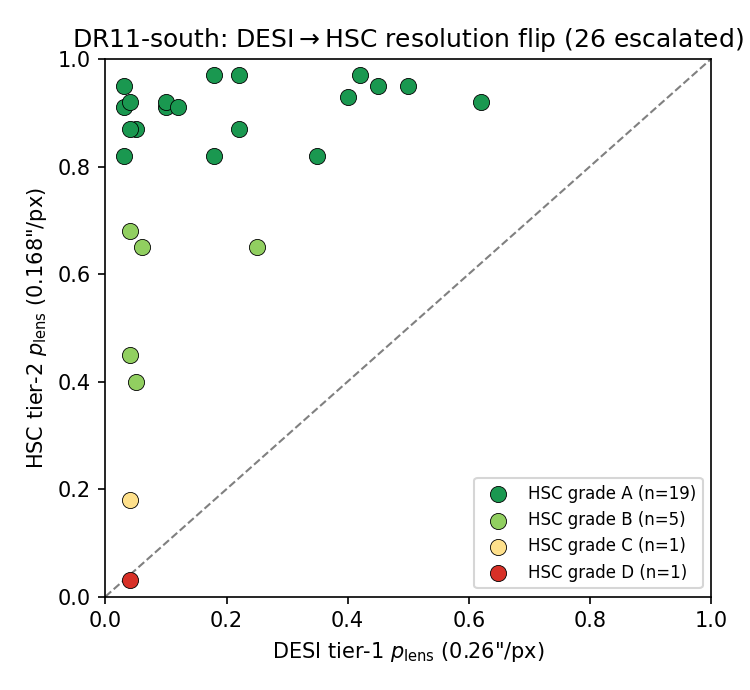
\includegraphics[width=0.49\linewidth]{figures/desi_hsc_flip.png}\hfill
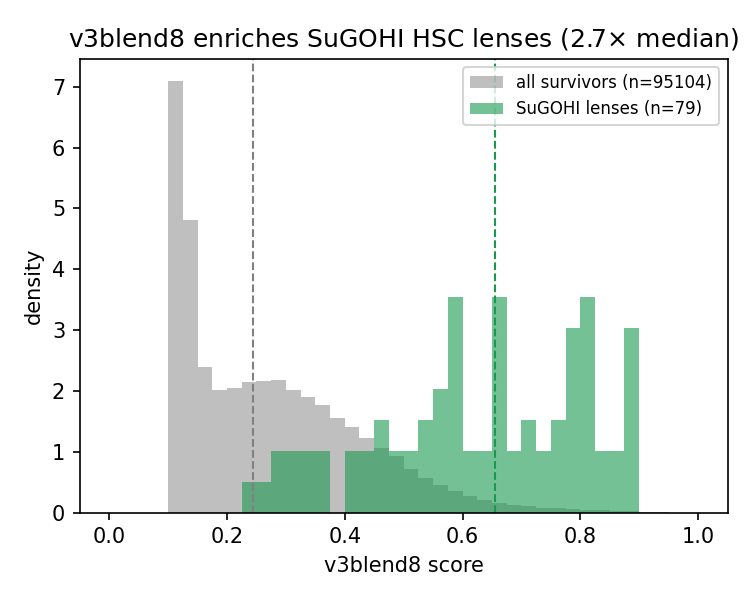
\includegraphics[width=0.49\linewidth]{figures/sugohi_enrichment.png}
\caption{Left: the DESI$\to$HSC resolution flip --- the 26 HSC-covered candidates move from
DESI-ambiguous (tier-1 $p_{\rm lens}$) to the HSC tier-2 grade (automated grader), 24 landing A/B above
the $y\!=\!x$ line. Right: \vb{} enriches the independent SuGOHI HSC lenses to $2.7\times$ the
survivor-median score (median lines dashed).}
\label{fig:flip}
\end{figure}

\paragraph{The resolution lever converts.} Every tier-2 grade-A/B candidate shows a large DESI$\to$HSC
flip: median tier-1 $p_{\rm lens}\!\approx\!0.1$ rising to tier-2 $0.82$--$0.97$ (e.g.\ $0.03\to0.95$,
$0.04\to0.92$). At DECaLS 1\arcsec\ seeing these are ambiguous (lrg+companion $\approx$ lens); at HSC
0.6\arcsec\ the arc/ring morphology resolves --- the flip is the grader's response to resolution, not
an observational confirmation.

\paragraph{Independent SuGOHI validation.} Against the SuGOHI/HOLISMOKES HSC committee lens catalog ---
an \emph{independent} sample with expert grades and spectroscopic redshifts \citep{sonnenfeld2018sugohi}
--- \vb{} recovers \textbf{79} lenses into the 95{,}104 survivors at a median \vb{} score $2.7\times$ the
survivor median (27 in the top-500), and \textbf{15 of the 24} tier-2 grade-A/B candidates are SuGOHI
lenses. These 15 are a \emph{sensitivity} check --- the automated HSC grader recovers known committee
lenses as grade-A/B --- but they do not establish its \emph{precision} on the genuinely-new candidates:
no negative control was run through tier-2 and the certified-FDR is power-limited (\S\ref{sec:sweep}),
so the false-positive rate of the new set is unquantified.

\paragraph{The candidate catalog.} Of the 24 tier-2 grade-A/B candidates, \textbf{0} are in the DESI
lens-finder catalogs (by construction --- the 500 were the new set after removing the 102 known), 15 are
SuGOHI cross-matches, and \textbf{9} (8 distinct systems) are new to the DESI finders and SuGOHI
(Table~\ref{tab:confirmed}). A post-hoc literature crosscheck --- Huang+2020 (omitted from the
campaign's lineage crossmatch) plus a NED/SIMBAD cone search (App.~\ref{app:gallery}) --- then shows
\textbf{five of these eight systems are previously-published lenses} (mostly Huang+2020; one also in the
SOAR Gravitational Arc Survey), leaving \textbf{3} genuinely new (\texttt{s\_327526\_9059},
\texttt{s\_340971\_2860}, \texttt{s\_325163\_2981}); the recoveries are an external validation of the
finder. The honest caveats: \lj{}'s HSC grading is automated (a single Claude grader, not a human
committee, no spectroscopy), and ``new'' here means new to the DESI finders, SuGOHI, \emph{and} the
NED/SIMBAD literature. They are candidates warranting human-expert and spectroscopic follow-up, not
confirmed lenses.

\begin{table}[t]\centering
\caption{The 9 HSC tier-2 grade-A/B candidate detections (8 distinct systems). A literature crosscheck
(Huang+2020 $+$ NED/SIMBAD; App.~\ref{app:gallery}) finds \textbf{5 systems are previously-published}
(\emph{known}: H20 $=$ Huang+2020; one also SOGRAS) and \textbf{3} genuinely new. $p_1,p_2$ = \lj{}
tier-1 (DESI) / tier-2 (HSC) lens probability.}
\label{tab:confirmed}
\begin{tabular}{lcccccl}
\toprule
name & RA & Dec & grade & $p_1\!\to\!p_2$ & \vb{} & known\\
\midrule
s\_340513\_3688 & 16.332 & $+1.749$  & A & $0.22\to0.97$ & 0.77 & Huang+2020\\
s\_327526\_9059 & 9.722  & $-0.409$  & A & $0.04\to0.92$ & 0.74 & \textbf{new}\\
s\_351303\_461  & 194.534& $+3.536$  & A & $0.62\to0.92$ & 0.89 & Huang+2020\\
s\_345385\_1515$^{\dagger}$ & 154.312 & $+2.489$ & A & $0.10\to0.92$ & 0.81 & Huang+2020\\
s\_340971\_2860 & 130.857& $+1.784$  & A & $0.12\to0.91$ & 0.76 & \textbf{new}\\
s\_345385\_1514$^{\dagger}$ & 154.312 & $+2.488$ & A & $0.05\to0.87$ & 0.86 & Huang+2020\\
s\_326089\_1785 & 10.288 & $-0.730$  & A & $0.03\to0.82$ & 0.83 & H20$+$SOGRAS\\
s\_325163\_2981 & 138.848& $-0.923$  & A & $0.18\to0.82$ & 0.74 & \textbf{new}\\
s\_318043\_1037 & 158.789& $-2.304$  & B & $0.04\to0.45$ & 0.86 & Huang+2020\\
\bottomrule
\end{tabular}

\smallskip
{\footnotesize $^{\dagger}$ s\_345385\_1514/1515 are adjacent ($\sim$1\arcsec) detections of the same
system, so the 9 detections are \textbf{8 distinct candidate systems} (8 A-detections / 7 distinct
grade-A + 1 grade-B).}
\end{table}

\paragraph{Active-learning loop.} The cascade's agent-confirmed mimics (grade-D $+$ named contaminant)
export to \textbf{291} hard negatives in the \cnet{} mimic-bank schema --- \texttt{lrg\_companion}
243-dominant, confirming that the high-\vb{} new frontier is lrg+companion-dominated at DECaLS
resolution (exactly the population the HSC tier-2 rejects). Folding these into the bank and a model
re-iteration are Perlmutter GPU work, deferred (below).

\section{DR11-north: staged, maintenance-deferred}
\label{sec:north}
v3 is DECam-specific --- it systematically under-scores BASS/MzLS north imaging --- so the north arm
requires instrument-native retraining. We built the full north parent (\textbf{$1.16\times10^{7}$}
galaxies, \emph{grz} only, no $i$), an 8-part manifest, and extracted \textbf{523} north-native
training positives (297 BASS/MzLS curated + 226 non-leaked catalog lenses; 86 clean held-out; 33 v1
leaks tracked); the retrainer is patched to fine-tune the three swappable members from their \texttt{\_b50}
checkpoints on a north-native mimic blend. A full-system Perlmutter maintenance (2026-06-17 to 06-24)
began mid-campaign before the north extraction could be scheduled, so the north sweep + retrain +
validation gates are \textbf{deferred to post-maintenance}; all inputs are staged for a clean resume.

\section{Conclusion}
On the final DESI Legacy Surveys release, the contaminant-aware \cnet{} finder plus the \lj{}~v3 HSC
cascade is a working DESI$\times$HSC cross-validation engine on the DECam-south footprint: it scores
$5.4\times10^{7}$ galaxies, recalibrates honestly to the DR11 domain shift (with a real $\sim$34\%
relative grade-A recall loss vs DR10 --- the survivor list is incomplete), and --- through the new
HSC tier-2 over a 20$\times$-wider footprint than Euclid Q1 --- moves 24 DESI-ambiguous candidates to
HSC tier-2 grade-A/B under \lj{}'s automated grader, of which 15 are SuGOHI committee lenses (a
sensitivity check) and 9 (8 systems) are new to the DESI finders and SuGOHI --- though a literature
crosscheck (Huang+2020 $+$ NED/SIMBAD; App.~\ref{app:gallery}) then shows 5 of those 8 systems are
previously-published lenses, leaving \textbf{3} genuinely new. The certified-FDR is power-limited
(zero) at full-population scale, the tier-2 grader is automated (no human committee or spectroscopy,
precision on the new set unquantified), and \emph{no net-new lens is established from DECaLS pixels
alone} --- the new candidate detections depend on HSC resolution and remain unconfirmed pending
follow-up. This is the same honest ceiling the v3 program established --- the resolution lever
\emph{converts} overlap candidates rather than manufacturing discoveries --- now measured on DR11 with a
much wider confirmable overlap. The north footprint, requiring instrument-native retraining, is staged
for completion after the Perlmutter maintenance window.

\bibliographystyle{plainnat}
\bibliography{references}

\clearpage
\appendix
\section{The new candidate systems at DESI and HSC resolution}
\label{app:gallery}
The figures below show the \textbf{8 distinct candidate systems} (the 9 detections of
Table~\ref{tab:confirmed}; the \texttt{s\_345385} pair is one system). A post-hoc literature crosscheck
(below) finds \textbf{5 of the 8 are previously-published lenses} (Huang+2020; one also SOGRAS) and
\textbf{3} are genuinely new. Each is rendered as: the
\cnet{}-seen DESI \emph{grz} cutout (0.262\arcsec/px, Lupton RGB --- what the finder scored, ambiguous
at DECaLS resolution); the HSC PDR3 \emph{grizy} cutout (0.168\arcsec/px --- the same view \lj{}'s
tier-2 grader inspected); and the HSC lens-light-subtracted view. The DESI$\to$HSC contrast is the
campaign's mechanism made visual: the finder ranks these high from ambiguous DECaLS pixels, and the
resolution lever reveals the arc/ring morphology (clearest in \texttt{s\_340513\_3688}; fainter and
correspondingly less certain in others). These are \emph{automated-grader candidates, not confirmed
lenses} --- they warrant human-expert and spectroscopic follow-up.
\noindent\emph{Literature crosscheck (added post-vetting).} The campaign's lineage
crossmatch omitted the Huang+2020 DECaLS catalogue and did not query the wider
literature. A full check --- Huang+2020 plus a NED/SIMBAD cone search --- finds that
\textbf{five of these eight systems are previously-published lenses} (flagged
\emph{Known} below; mostly Huang+2020, one also in the SOAR Gravitational Arc
Survey). Only \texttt{s\_327526\_9059}, \texttt{s\_340971\_2860}, and
\texttt{s\_325163\_2981} are genuinely new (absent from the lineage \emph{and} the
literature). The recoveries are an external validation of the v3$+$cascade finder;
the net-new count here is \textbf{3}, not 8.\par\smallskip

\begin{figure}[ht]\centering
\begin{minipage}[b]{0.32\linewidth}\centering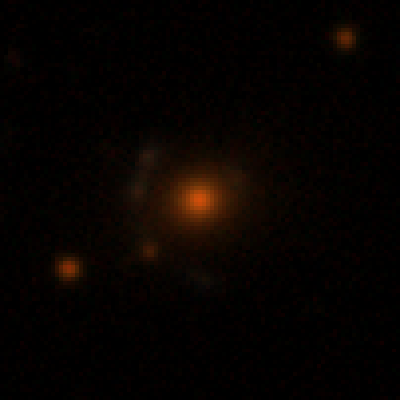
\includegraphics[width=\linewidth]{figures/cand_s_340513_3688_desi.png}\\[2pt]{\scriptsize DESI \emph{grz} (0.262\arcsec/px)}\end{minipage}\hfill
\begin{minipage}[b]{0.32\linewidth}\centering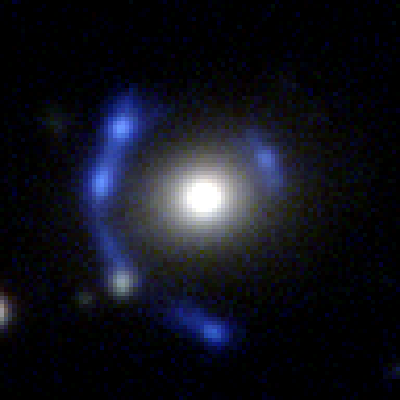
\includegraphics[width=\linewidth]{figures/cand_s_340513_3688_hsc.png}\\[2pt]{\scriptsize HSC \emph{grizy} (0.168\arcsec/px)}\end{minipage}\hfill
\begin{minipage}[b]{0.32\linewidth}\centering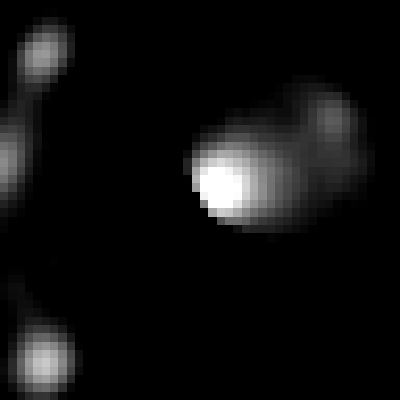
\includegraphics[width=\linewidth]{figures/cand_s_340513_3688_hscsub.png}\\[2pt]{\scriptsize HSC lens-light subtracted}\end{minipage}
\caption{\texttt{s\_340513\_3688} (RA 16.3319, Dec +1.7490) --- HSC tier-2 grade \textbf{A}, $p_{\rm lens}$ 0.22$\to$0.97, \vb{} 0.77. \emph{Known}: Huang+2020 \texttt{DESI-016.3319+01.7490} (grade A), $0.1\arcsec$.}
\end{figure}
\begin{figure}[ht]\centering
\begin{minipage}[b]{0.32\linewidth}\centering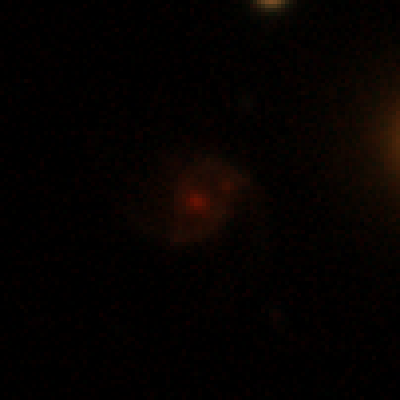
\includegraphics[width=\linewidth]{figures/cand_s_327526_9059_desi.png}\\[2pt]{\scriptsize DESI \emph{grz} (0.262\arcsec/px)}\end{minipage}\hfill
\begin{minipage}[b]{0.32\linewidth}\centering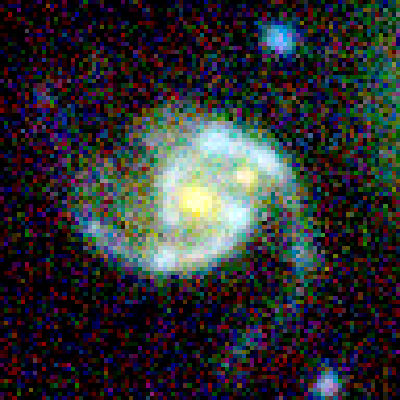
\includegraphics[width=\linewidth]{figures/cand_s_327526_9059_hsc.png}\\[2pt]{\scriptsize HSC \emph{grizy} (0.168\arcsec/px)}\end{minipage}\hfill
\begin{minipage}[b]{0.32\linewidth}\centering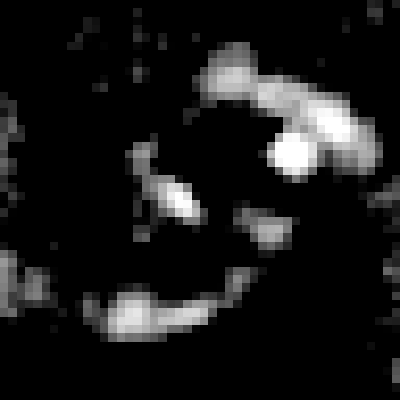
\includegraphics[width=\linewidth]{figures/cand_s_327526_9059_hscsub.png}\\[2pt]{\scriptsize HSC lens-light subtracted}\end{minipage}
\caption{\texttt{s\_327526\_9059} (RA 9.7222, Dec -0.4093) --- HSC tier-2 grade \textbf{A}, $p_{\rm lens}$ 0.04$\to$0.92, \vb{} 0.74. \emph{New}: absent from the lineage and from NED/SIMBAD.}
\end{figure}
\begin{figure}[ht]\centering
\begin{minipage}[b]{0.32\linewidth}\centering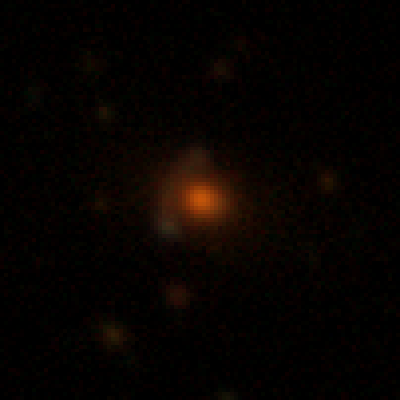
\includegraphics[width=\linewidth]{figures/cand_s_351303_461_desi.png}\\[2pt]{\scriptsize DESI \emph{grz} (0.262\arcsec/px)}\end{minipage}\hfill
\begin{minipage}[b]{0.32\linewidth}\centering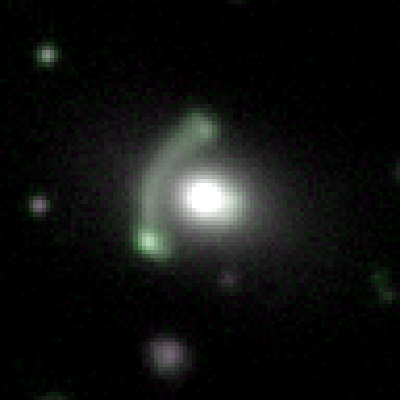
\includegraphics[width=\linewidth]{figures/cand_s_351303_461_hsc.png}\\[2pt]{\scriptsize HSC \emph{grizy} (0.168\arcsec/px)}\end{minipage}\hfill
\begin{minipage}[b]{0.32\linewidth}\centering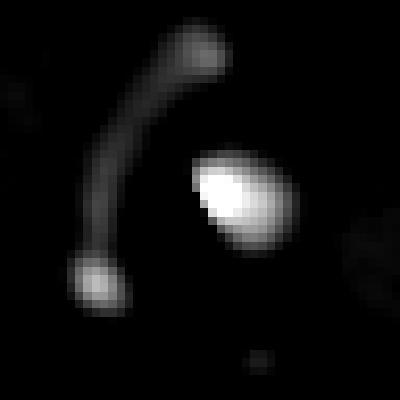
\includegraphics[width=\linewidth]{figures/cand_s_351303_461_hscsub.png}\\[2pt]{\scriptsize HSC lens-light subtracted}\end{minipage}
\caption{\texttt{s\_351303\_461} (RA 194.5345, Dec +3.5358) --- HSC tier-2 grade \textbf{A}, $p_{\rm lens}$ 0.62$\to$0.92, \vb{} 0.89. \emph{Known}: Huang+2020 \texttt{DESI-194.5344+03.5358} (grade A), $0.2\arcsec$.}
\end{figure}
\begin{figure}[ht]\centering
\begin{minipage}[b]{0.32\linewidth}\centering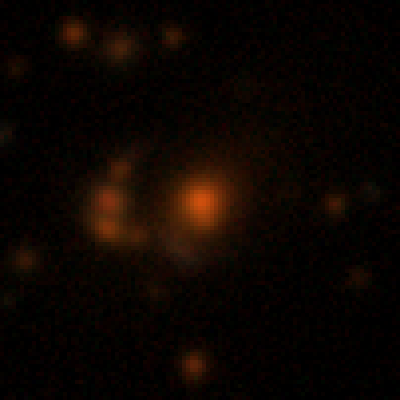
\includegraphics[width=\linewidth]{figures/cand_s_345385_1515_desi.png}\\[2pt]{\scriptsize DESI \emph{grz} (0.262\arcsec/px)}\end{minipage}\hfill
\begin{minipage}[b]{0.32\linewidth}\centering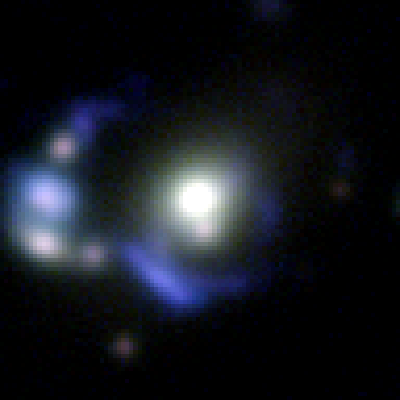
\includegraphics[width=\linewidth]{figures/cand_s_345385_1515_hsc.png}\\[2pt]{\scriptsize HSC \emph{grizy} (0.168\arcsec/px)}\end{minipage}\hfill
\begin{minipage}[b]{0.32\linewidth}\centering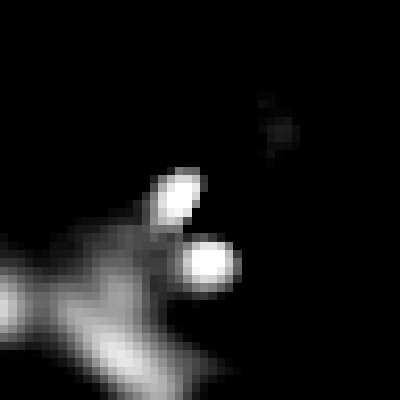
\includegraphics[width=\linewidth]{figures/cand_s_345385_1515_hscsub.png}\\[2pt]{\scriptsize HSC lens-light subtracted}\end{minipage}
\caption{\texttt{s\_345385\_1515} (RA 154.3116, Dec +2.4885) --- HSC tier-2 grade \textbf{A}, $p_{\rm lens}$ 0.10$\to$0.92, \vb{} 0.81. \emph{Known}: Huang+2020 \texttt{DESI-154.3116+02.4885} (grade C), $0.1\arcsec$. (= 8th detection s\_345385\_1514, the adjacent $\sim$1\arcsec\ pair, omitted)}
\end{figure}
\begin{figure}[ht]\centering
\begin{minipage}[b]{0.32\linewidth}\centering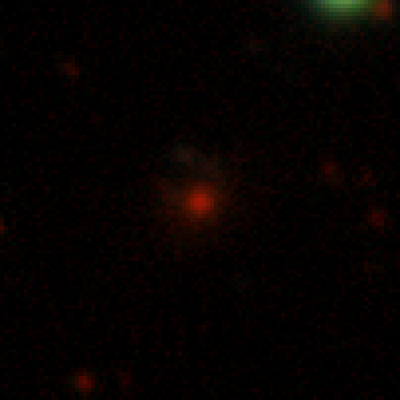
\includegraphics[width=\linewidth]{figures/cand_s_340971_2860_desi.png}\\[2pt]{\scriptsize DESI \emph{grz} (0.262\arcsec/px)}\end{minipage}\hfill
\begin{minipage}[b]{0.32\linewidth}\centering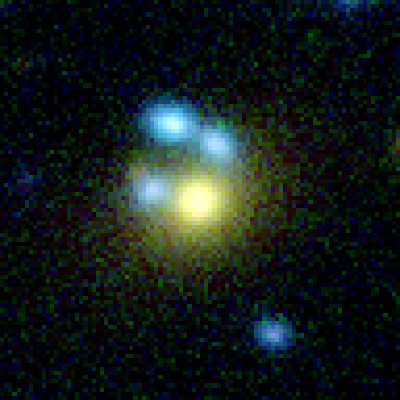
\includegraphics[width=\linewidth]{figures/cand_s_340971_2860_hsc.png}\\[2pt]{\scriptsize HSC \emph{grizy} (0.168\arcsec/px)}\end{minipage}\hfill
\begin{minipage}[b]{0.32\linewidth}\centering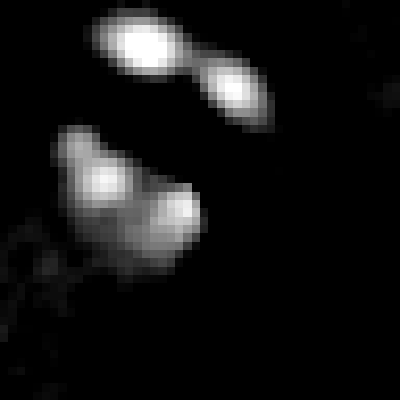
\includegraphics[width=\linewidth]{figures/cand_s_340971_2860_hscsub.png}\\[2pt]{\scriptsize HSC lens-light subtracted}\end{minipage}
\caption{\texttt{s\_340971\_2860} (RA 130.8571, Dec +1.7840) --- HSC tier-2 grade \textbf{A}, $p_{\rm lens}$ 0.12$\to$0.91, \vb{} 0.76. \emph{New}: absent from the lineage and from NED/SIMBAD.}
\end{figure}
\begin{figure}[ht]\centering
\begin{minipage}[b]{0.32\linewidth}\centering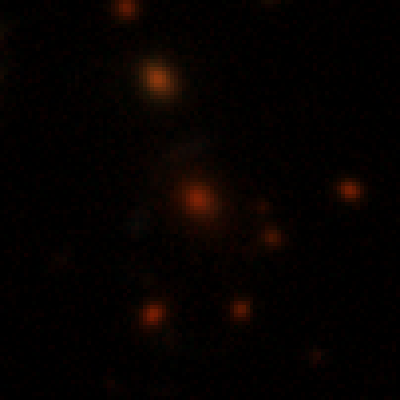
\includegraphics[width=\linewidth]{figures/cand_s_326089_1785_desi.png}\\[2pt]{\scriptsize DESI \emph{grz} (0.262\arcsec/px)}\end{minipage}\hfill
\begin{minipage}[b]{0.32\linewidth}\centering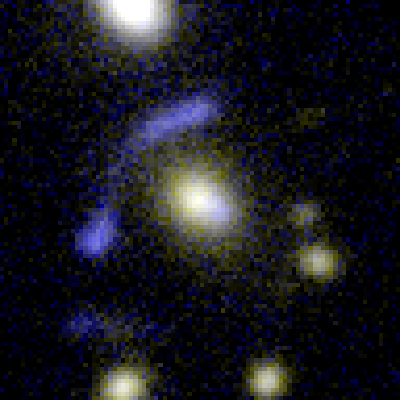
\includegraphics[width=\linewidth]{figures/cand_s_326089_1785_hsc.png}\\[2pt]{\scriptsize HSC \emph{grizy} (0.168\arcsec/px)}\end{minipage}\hfill
\begin{minipage}[b]{0.32\linewidth}\centering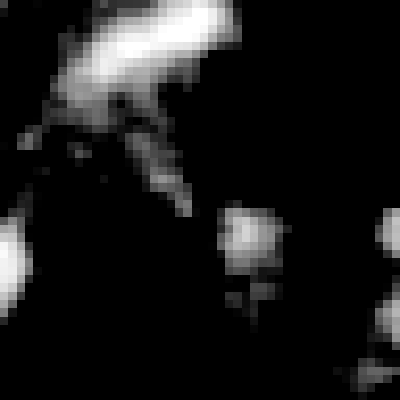
\includegraphics[width=\linewidth]{figures/cand_s_326089_1785_hscsub.png}\\[2pt]{\scriptsize HSC lens-light subtracted}\end{minipage}
\caption{\texttt{s\_326089\_1785} (RA 10.2876, Dec -0.7303) --- HSC tier-2 grade \textbf{A}, $p_{\rm lens}$ 0.03$\to$0.82, \vb{} 0.83. \emph{Known}: Huang+2020 \texttt{DESI-010.2876-00.7303} (grade B), also SOGRAS~J0041$-$0043, $0.1\arcsec$.}
\end{figure}
\begin{figure}[ht]\centering
\begin{minipage}[b]{0.32\linewidth}\centering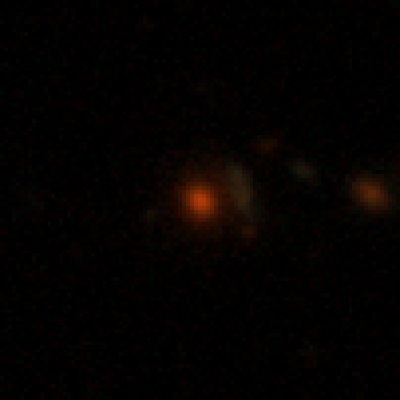
\includegraphics[width=\linewidth]{figures/cand_s_325163_2981_desi.png}\\[2pt]{\scriptsize DESI \emph{grz} (0.262\arcsec/px)}\end{minipage}\hfill
\begin{minipage}[b]{0.32\linewidth}\centering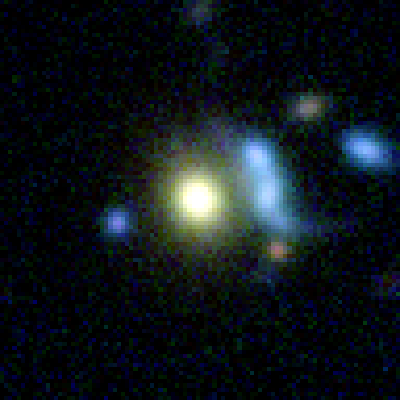
\includegraphics[width=\linewidth]{figures/cand_s_325163_2981_hsc.png}\\[2pt]{\scriptsize HSC \emph{grizy} (0.168\arcsec/px)}\end{minipage}\hfill
\begin{minipage}[b]{0.32\linewidth}\centering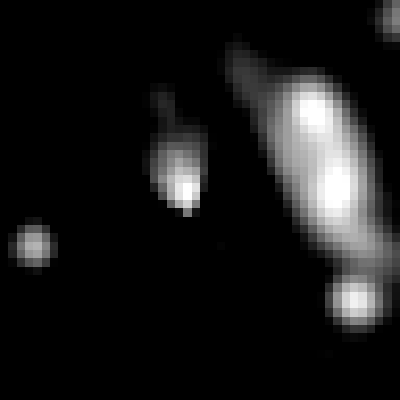
\includegraphics[width=\linewidth]{figures/cand_s_325163_2981_hscsub.png}\\[2pt]{\scriptsize HSC lens-light subtracted}\end{minipage}
\caption{\texttt{s\_325163\_2981} (RA 138.8482, Dec -0.9226) --- HSC tier-2 grade \textbf{A}, $p_{\rm lens}$ 0.18$\to$0.82, \vb{} 0.74. \emph{New}: absent from the lineage and from NED/SIMBAD.}
\end{figure}
\begin{figure}[ht]\centering
\begin{minipage}[b]{0.32\linewidth}\centering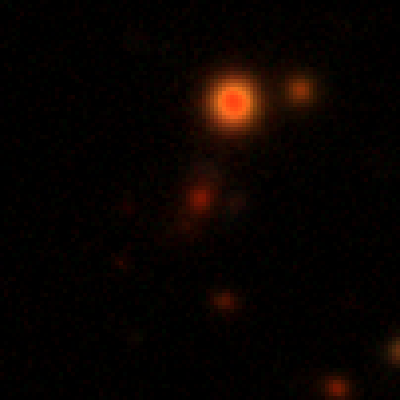
\includegraphics[width=\linewidth]{figures/cand_s_318043_1037_desi.png}\\[2pt]{\scriptsize DESI \emph{grz} (0.262\arcsec/px)}\end{minipage}\hfill
\begin{minipage}[b]{0.32\linewidth}\centering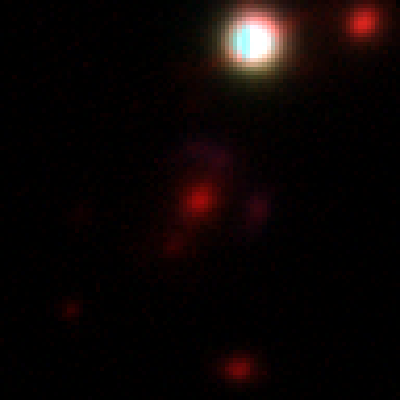
\includegraphics[width=\linewidth]{figures/cand_s_318043_1037_hsc.png}\\[2pt]{\scriptsize HSC \emph{grizy} (0.168\arcsec/px)}\end{minipage}\hfill
\begin{minipage}[b]{0.32\linewidth}\centering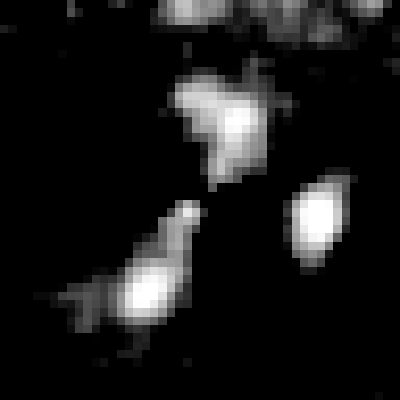
\includegraphics[width=\linewidth]{figures/cand_s_318043_1037_hscsub.png}\\[2pt]{\scriptsize HSC lens-light subtracted}\end{minipage}
\caption{\texttt{s\_318043\_1037} (RA 158.7893, Dec -2.3037) --- HSC tier-2 grade \textbf{B}, $p_{\rm lens}$ 0.04$\to$0.45, \vb{} 0.86. \emph{Known}: Huang+2020 \texttt{DESI-158.7893-02.3037} (grade B), $0.1\arcsec$.}
\end{figure}


\clearpage
\section{DESI-resolution candidates without high-resolution coverage}
\label{app:resolution}
Only $\sim$7\% of the DR11-south candidates fall in HSC-SSP (\S\ref{sec:vet}); the rest cannot be
validated beyond DECaLS resolution with current high-res data. Table~\ref{tab:resolution} lists all
\textbf{78} candidates graded A/B at DECaLS $1\arcsec$ by the LensJudge cascade that are \emph{not} in
HSC-SSP \emph{or} Euclid~Q1 (8~A, 70~B), ranked by tier-1 $p_{\rm lens}$, with DESI \emph{grz} cutouts
in Figs.~\ref{fig:resgal1}--\ref{fig:resgal2}. A literature crosscheck (\texttt{crosscheck\_candidates.py};
Huang/Storfer/Inchausti $+$ NED/SIMBAD) finds \textbf{53 of the 78 are previously-published lenses} ---
38 from the Dark Energy Survey lens searches, 8 Huang+2020, 6 AGEL, 1 CASSOWARY (the \emph{known} column
of Table~\ref{tab:resolution}) --- because this DECaLS-south footprint heavily overlaps DES, which the
campaign crossmatch omitted; the \textbf{25 genuinely new} are all grade~B (the 8 grade-A are all known
lenses). A follow-up NED cone search corroborates the new set (no NED lens match; 24/25 returned, one
NED timeout). At $1\arcsec$ a genuine lens and an lrg+companion mimic
are not separable (the resolution ceiling of \S\ref{sec:vet}), so these are \emph{candidates}, an
unknown and likely large fraction of which are mimics --- the contact sheets show both clear arc/ring
morphologies and ambiguous lrg+companion configurations. They are listed in full for completeness and
as a follow-up target set, awaiting Euclid~DR1 / Rubin / Roman or targeted high-resolution and
spectroscopic follow-up.
\begin{longtable}{rlcccccc}
\caption{The 108 DESI-resolution grade-A/B candidates (LensJudge \texttt{direct/escalate} grade at DECaLS $0.262\arcsec$) with \emph{no} HSC-SSP or Euclid~Q1 coverage, ranked by tier-1 $p_{\rm lens}$. A literature crosscheck (\texttt{crosscheck\_candidates.py}: the Huang/Storfer/Inchausti catalogues $+$ a NED/SIMBAD cone search) finds \textbf{69 are previously-published lenses} --- 48~DES, 11~Huang+2020, 6~AGEL, 3~SIMBAD, 1~CASSOWARY (\emph{known} column: survey code; per-object matches in \texttt{data/dr11s\_resolution\_xmatch.csv}) --- and \textbf{39 are genuinely new} (\,---\,; 3 grade~A and 36 grade~B). The high known fraction is because this DECaLS-south footprint heavily overlaps the Dark Energy Survey lens searches, which the campaign crossmatch omitted. The new ones cannot be validated beyond DECaLS resolution; at $1\arcsec$ a genuine lens and an lrg+companion mimic are not separable, so an unknown fraction are mimics. Per-candidate full/zoom/residual panels follow (App.~\ref{app:resolution}).}\\
\label{tab:resolution}\\
\toprule
\# & name & RA & Dec & grade & $p_{\rm lens}$ & \vb{} & known \\
\midrule
\endfirsthead
\multicolumn{8}{l}{\footnotesize Table~\ref{tab:resolution} continued}\\
\toprule
\# & name & RA & Dec & grade & $p_{\rm lens}$ & \vb{} & known \\
\midrule
\endhead
\midrule\multicolumn{8}{r}{\footnotesize continued\ldots}\\
\endfoot
\bottomrule
\endlastfoot
1 & \texttt{s\_441355\_1188} & 177.1381 & +19.5009 & A & 0.95 & 0.83 & CSWA \\
2 & \texttt{s\_98012\_247} & 56.1462 & -44.7956 & A & 0.92 & 0.86 & DES \\
3 & \texttt{s\_310364\_6388} & 38.2078 & -3.3906 & A & 0.88 & 0.82 & H20 \\
4 & \texttt{s\_301694\_7426} & 26.2679 & -4.9310 & A & 0.88 & 0.85 & H20 \\
5 & \texttt{s\_181942\_4122} & 61.6016 & -26.7733 & A & 0.87 & 0.86 & DES \\
6 & \texttt{s\_137502\_1047} & 26.4450 & -35.6910 & A & 0.87 & 0.80 & DES \\
7 & \texttt{s\_230539\_4159} & 222.0715 & -17.8489 & A & 0.85 & 0.84 & \,--- \\
8 & \texttt{s\_71042\_1653} & 20.1760 & -51.7314 & A & 0.85 & 0.82 & DES \\
9 & \texttt{s\_180593\_5604} & 44.0974 & -27.1218 & A & 0.85 & 0.88 & DES \\
10 & \texttt{s\_194300\_2796} & 242.6052 & -24.4155 & A & 0.83 & 0.74 & \,--- \\
11 & \texttt{s\_304994\_4662} & 133.5531 & -4.4026 & A & 0.82 & 0.84 & H20 \\
12 & \texttt{s\_61472\_9399} & 359.5200 & -54.6765 & A & 0.80 & 0.88 & DES \\
13 & \texttt{s\_91761\_4679} & 350.3683 & -46.5138 & A & 0.80 & 0.86 & DES \\
14 & \texttt{s\_91796\_2958} & 2.9714 & -46.2395 & A & 0.78 & 0.79 & DES \\
15 & \texttt{s\_320069\_835} & 305.2638 & -1.9376 & A & 0.78 & 0.89 & \,--- \\
16 & \texttt{s\_292418\_3907} & 216.8280 & -6.7541 & A & 0.78 & 0.89 & H20 \\
17 & \texttt{s\_81254\_12458} & 57.3313 & -48.9592 & A & 0.76 & 0.84 & DES \\
18 & \texttt{s\_124958\_7349} & 58.1768 & -38.4292 & B & 0.68 & 0.89 & DES \\
19 & \texttt{s\_59958\_9730} & 64.5412 & -54.9597 & B & 0.65 & 0.83 & DES \\
20 & \texttt{s\_197474\_9756} & 30.7668 & -23.6341 & B & 0.65 & 0.81 & DES \\
21 & \texttt{s\_313198\_1471} & 27.5380 & -3.0773 & B & 0.65 & 0.81 & AGEL \\
22 & \texttt{s\_232538\_8716} & 25.2755 & -17.2232 & B & 0.65 & 0.85 & H20 \\
23 & \texttt{s\_280236\_3353} & 25.8623 & -8.8393 & B & 0.65 & 0.84 & AGEL \\
24 & \texttt{s\_234689\_542} & 227.0427 & -16.8771 & B & 0.65 & 0.80 & \,--- \\
25 & \texttt{s\_502450\_1680} & 161.1145 & +31.2344 & B & 0.63 & 0.79 & \,--- \\
26 & \texttt{s\_94959\_7228} & 56.8054 & -45.5850 & B & 0.62 & 0.84 & DES \\
27 & \texttt{s\_119342\_4136} & 50.7164 & -39.7694 & B & 0.62 & 0.90 & DES \\
28 & \texttt{s\_243378\_3831} & 326.5170 & -15.4964 & B & 0.62 & 0.84 & \,--- \\
29 & \texttt{s\_240846\_8850} & 30.2832 & -15.8547 & B & 0.62 & 0.80 & H20 \\
30 & \texttt{s\_188493\_9685} & 83.4556 & -25.6151 & B & 0.62 & 0.88 & DES \\
31 & \texttt{s\_94933\_7964} & 47.5548 & -45.5743 & B & 0.60 & 0.78 & DES \\
32 & \texttt{s\_95070\_5466} & 96.2505 & -45.4358 & B & 0.60 & 0.78 & DES \\
33 & \texttt{s\_369309\_653} & 30.4465 & +6.6551 & B & 0.60 & 0.74 & \,--- \\
34 & \texttt{s\_34114\_11363} & 353.7468 & -64.0687 & B & 0.58 & 0.90 & DES \\
35 & \texttt{s\_102952\_10164} & 334.8017 & -43.8098 & B & 0.58 & 0.85 & DES \\
36 & \texttt{s\_191004\_9637} & 56.9356 & -24.9088 & B & 0.58 & 0.88 & DES \\
37 & \texttt{s\_43736\_6056} & 67.3945 & -60.1905 & B & 0.58 & 0.83 & DES \\
38 & \texttt{s\_137518\_1133} & 31.3588 & -35.6632 & B & 0.58 & 0.84 & DES \\
39 & \texttt{s\_129372\_3768} & 16.4504 & -37.4286 & B & 0.58 & 0.82 & DES \\
40 & \texttt{s\_98882\_7820} & 1.6860 & -44.4974 & B & 0.58 & 0.80 & DES \\
41 & \texttt{s\_218735\_721} & 350.2028 & -20.0497 & B & 0.58 & 0.79 & \,--- \\
42 & \texttt{s\_360639\_3636} & 13.4868 & +5.3590 & B & 0.55 & 0.85 & \,--- \\
43 & \texttt{s\_381188\_1199} & 144.1511 & +8.8633 & B & 0.55 & 0.90 & H20 \\
44 & \texttt{s\_114736\_1046} & 343.5127 & -40.9303 & B & 0.55 & 0.86 & DES \\
45 & \texttt{s\_87091\_1800} & 84.5193 & -47.5872 & B & 0.55 & 0.89 & DES \\
46 & \texttt{s\_327710\_4950} & 55.6649 & -0.3820 & B & 0.55 & 0.74 & \,--- \\
47 & \texttt{s\_289350\_3716} & 164.8051 & -7.1449 & B & 0.55 & 0.81 & \,--- \\
48 & \texttt{s\_384032\_2232} & 143.3887 & +9.3219 & B & 0.55 & 0.84 & H20 \\
49 & \texttt{s\_73683\_6069} & 357.3753 & -51.2276 & B & 0.55 & 0.83 & DES \\
50 & \texttt{s\_80200\_6872} & 15.4919 & -49.2940 & B & 0.55 & 0.88 & DES \\
51 & \texttt{s\_58263\_3751} & 42.7179 & -55.4032 & B & 0.55 & 0.88 & DES \\
52 & \texttt{s\_491286\_1438} & 180.3616 & +29.0116 & B & 0.52 & 0.74 & \,--- \\
53 & \texttt{s\_164140\_7181} & 41.2060 & -30.3214 & B & 0.50 & 0.79 & DES \\
54 & \texttt{s\_71871\_246} & 353.9664 & -51.8716 & B & 0.50 & 0.76 & AGEL \\
55 & \texttt{s\_61626\_1035} & 65.1782 & -54.3770 & B & 0.50 & 0.87 & DES \\
56 & \texttt{s\_262449\_2840} & 188.7861 & -11.9798 & B & 0.50 & 0.87 & \,--- \\
57 & \texttt{s\_107312\_5223} & 23.8451 & -42.5398 & B & 0.50 & 0.85 & DES \\
58 & \texttt{s\_90920\_9419} & 45.9517 & -46.4407 & B & 0.50 & 0.85 & DES \\
59 & \texttt{s\_217461\_3974} & 12.0451 & -19.9206 & B & 0.50 & 0.78 & \,--- \\
60 & \texttt{s\_260341\_325} & 9.9798 & -12.2097 & B & 0.50 & 0.84 & \,--- \\
61 & \texttt{s\_207576\_2272} & 248.1195 & -22.0355 & B & 0.48 & 0.76 & \,--- \\
62 & \texttt{s\_162970\_1777} & 62.5554 & -30.6238 & B & 0.48 & 0.82 & DES \\
63 & \texttt{s\_234043\_6467} & 58.4427 & -17.1109 & B & 0.47 & 0.88 & AGEL \\
64 & \texttt{s\_283917\_2408} & 235.6200 & -8.3490 & B & 0.45 & 0.89 & \,--- \\
65 & \texttt{s\_50907\_11900} & 303.5808 & -57.9504 & B & 0.45 & 0.74 & DES \\
66 & \texttt{s\_61411\_4481} & 332.9866 & -54.6445 & B & 0.45 & 0.76 & DES \\
67 & \texttt{s\_165468\_9648} & 64.7771 & -29.9937 & B & 0.45 & 0.78 & DES \\
68 & \texttt{s\_148704\_6732} & 183.8176 & -33.6006 & B & 0.45 & 0.80 & \,--- \\
69 & \texttt{s\_280264\_9147} & 33.1051 & -8.8697 & B & 0.45 & 0.84 & literature (SIMBAD) \\
70 & \texttt{s\_266046\_1185} & 25.9989 & -11.2770 & B & 0.45 & 0.76 & \,--- \\
71 & \texttt{s\_251013\_4202} & 137.4230 & -13.9601 & B & 0.45 & 0.79 & \,--- \\
72 & \texttt{s\_52008\_8091} & 96.5963 & -57.5083 & B & 0.45 & 0.89 & DES \\
73 & \texttt{s\_209853\_1103} & 139.8053 & -21.4604 & B & 0.45 & 0.85 & \,--- \\
74 & \texttt{s\_504880\_4027} & 152.0763 & +31.7005 & B & 0.45 & 0.84 & H20 \\
75 & \texttt{s\_181762\_9592} & 11.4347 & -26.6294 & B & 0.45 & 0.86 & \,--- \\
76 & \texttt{s\_69087\_268} & 307.2325 & -52.5218 & B & 0.43 & 0.81 & DES \\
77 & \texttt{s\_256199\_9097} & 29.6819 & -13.0258 & B & 0.42 & 0.78 & DES \\
78 & \texttt{s\_36700\_530} & 347.9904 & -63.1176 & B & 0.42 & 0.78 & literature (SIMBAD) \\
79 & \texttt{s\_23764\_4161} & 132.6603 & -68.1876 & B & 0.42 & 0.79 & \,--- \\
80 & \texttt{s\_29019\_24056} & 248.9430 & -66.0747 & B & 0.42 & 0.74 & \,--- \\
81 & \texttt{s\_204169\_8722} & 49.1618 & -22.6093 & B & 0.42 & 0.77 & DES \\
82 & \texttt{s\_112158\_2867} & 209.6741 & -41.4932 & B & 0.42 & 0.83 & \,--- \\
83 & \texttt{s\_139825\_11098} & 18.9226 & -35.3386 & B & 0.42 & 0.76 & literature (SIMBAD) \\
84 & \texttt{s\_60524\_3113} & 309.7973 & -54.9952 & B & 0.42 & 0.81 & DES \\
85 & \texttt{s\_38835\_314} & 56.6543 & -61.9792 & B & 0.42 & 0.84 & DES \\
86 & \texttt{s\_405220\_1292} & 136.4655 & +13.0307 & B & 0.42 & 0.89 & \,--- \\
87 & \texttt{s\_68464\_11443} & 52.7373 & -52.4703 & B & 0.42 & 0.88 & DES \\
88 & \texttt{s\_206743\_10995} & 24.2120 & -22.0076 & B & 0.42 & 0.85 & DES \\
89 & \texttt{s\_41562\_4180} & 42.2402 & -60.9010 & B & 0.40 & 0.87 & DES \\
90 & \texttt{s\_188312\_3322} & 33.2537 & -25.3945 & B & 0.40 & 0.76 & \,--- \\
91 & \texttt{s\_120781\_3317} & 156.8525 & -39.6093 & B & 0.40 & 0.83 & \,--- \\
92 & \texttt{s\_266620\_918} & 172.1320 & -11.3108 & B & 0.40 & 0.80 & \,--- \\
93 & \texttt{s\_410935\_2097} & 164.1204 & +14.0606 & B & 0.38 & 0.83 & \,--- \\
94 & \texttt{s\_32666\_26056} & 248.6090 & -64.5569 & B & 0.38 & 0.73 & \,--- \\
95 & \texttt{s\_244220\_4253} & 184.3042 & -15.2610 & B & 0.38 & 0.80 & \,--- \\
96 & \texttt{s\_119499\_8020} & 101.8093 & -39.8359 & B & 0.38 & 0.75 & \,--- \\
97 & \texttt{s\_156771\_3446} & 54.3219 & -31.8704 & B & 0.38 & 0.89 & AGEL \\
98 & \texttt{s\_205319\_6061} & 359.9772 & -22.4596 & B & 0.38 & 0.88 & \,--- \\
99 & \texttt{s\_416616\_6090} & 189.5370 & +15.0309 & B & 0.38 & 0.93 & H20 \\
100 & \texttt{s\_364281\_4525} & 207.3133 & +5.6308 & B & 0.35 & 0.90 & \,--- \\
101 & \texttt{s\_250611\_2161} & 33.7898 & -14.1185 & B & 0.35 & 0.77 & \,--- \\
102 & \texttt{s\_212207\_5081} & 50.6597 & -20.9567 & B & 0.35 & 0.84 & \,--- \\
103 & \texttt{s\_128091\_3374} & 332.6355 & -37.9263 & B & 0.35 & 0.85 & \,--- \\
104 & \texttt{s\_194944\_4494} & 59.2045 & -24.1447 & B & 0.35 & 0.85 & DES \\
105 & \texttt{s\_94861\_9433} & 21.9716 & -45.5428 & B & 0.32 & 0.87 & DES \\
106 & \texttt{s\_235253\_4230} & 14.4452 & -16.7457 & B & 0.32 & 0.76 & H20 \\
107 & \texttt{s\_394431\_6727} & 261.7637 & +11.0021 & B & 0.30 & 0.77 & AGEL \\
108 & \texttt{s\_369977\_4434} & 198.5174 & +6.6887 & B & 0.28 & 0.75 & \,--- \\
\end{longtable}

\definecolor{forestgreen}{HTML}{157f15}
\subsection*{\textcolor{gray}{\textsc{Known}} --- previously-published lenses recovered (53 of 78)}
These coincide ($\le$few\,\arcsec) with a catalogued strong lens --- 38 DES, 8 Huang+2020, 6 AGEL, 1 CASSOWARY --- an external validation of the finder (the campaign crossmatch had omitted these catalogues). Ranked by tier-1 $p_{\rm lens}$.\par\smallskip
\begin{figure}[H]\centering
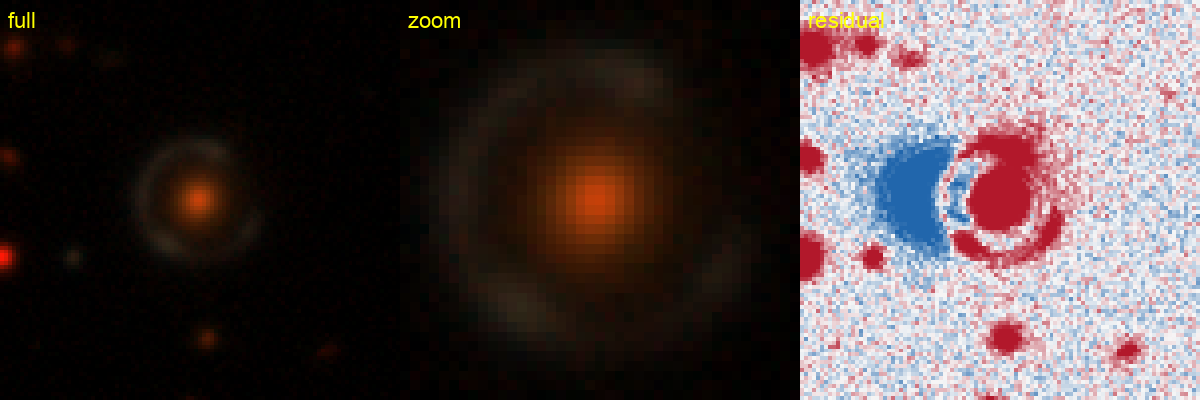
\includegraphics[width=\linewidth]{figures/res_s_310364_6388.png}
\caption{\textbf{\#1}~\texttt{s\_310364\_6388} --- RA 38.2078, Dec -3.3906; grade \textbf{A}, tier-1 $p_{\rm lens}$ 0.90, \vb{} 0.82. \textcolor{gray}{\textbf{KNOWN}} --- Huang+2020: \texttt{DESI-038.2078-03.3906}, $0.16\arcsec$ (lineage).}
\end{figure}
\begin{figure}[H]\centering
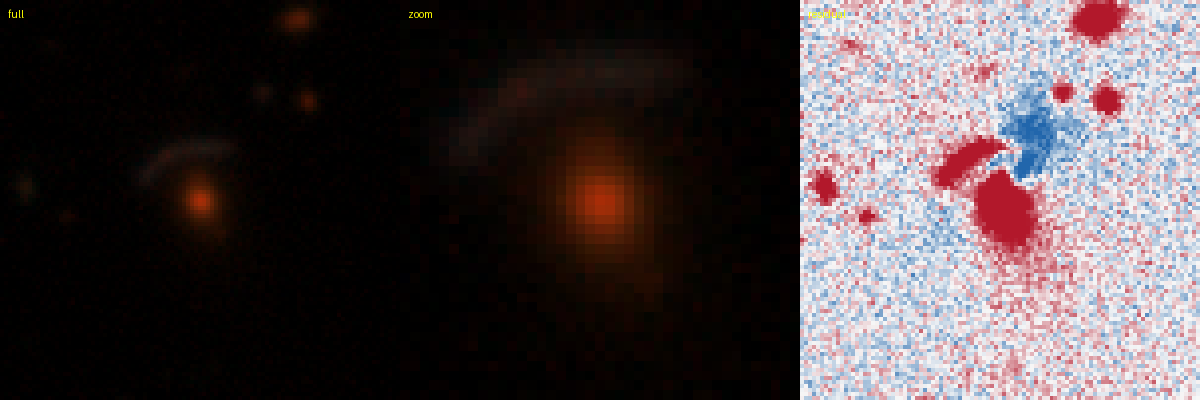
\includegraphics[width=\linewidth]{figures/res_s_137502_1047.png}
\caption{\textbf{\#2}~\texttt{s\_137502\_1047} --- RA 26.4450, Dec -35.6910; grade \textbf{A}, tier-1 $p_{\rm lens}$ 0.90, \vb{} 0.80. \textcolor{gray}{\textbf{KNOWN}} --- DES: \texttt{DES J014546.78-354127.3}, $0.20\arcsec$ (SIMBAD).}
\end{figure}
\begin{figure}[H]\centering
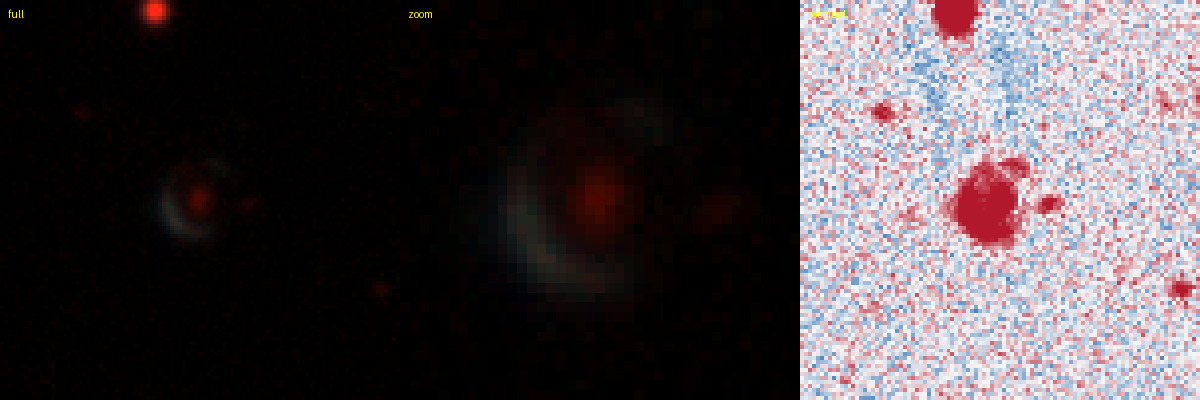
\includegraphics[width=\linewidth]{figures/res_s_181942_4122.png}
\caption{\textbf{\#3}~\texttt{s\_181942\_4122} --- RA 61.6016, Dec -26.7733; grade \textbf{A}, tier-1 $p_{\rm lens}$ 0.87, \vb{} 0.86. \textcolor{gray}{\textbf{KNOWN}} --- DES: \texttt{DES J040624.49-264625.0}, $1.74\arcsec$ (SIMBAD).}
\end{figure}
\begin{figure}[H]\centering
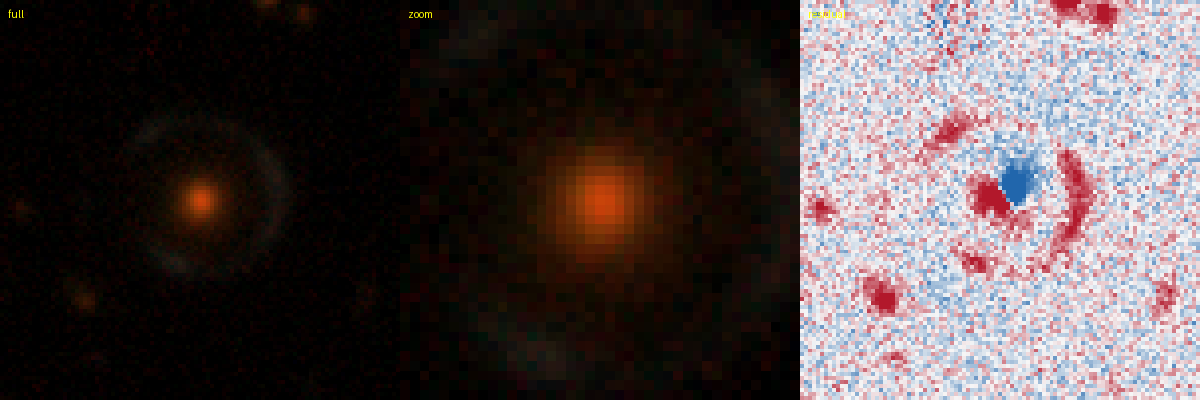
\includegraphics[width=\linewidth]{figures/res_s_441355_1188.png}
\caption{\textbf{\#4}~\texttt{s\_441355\_1188} --- RA 177.1381, Dec +19.5009; grade \textbf{A}, tier-1 $p_{\rm lens}$ 0.87, \vb{} 0.83. \textcolor{gray}{\textbf{KNOWN}} --- CASSOWARY: \texttt{CSWA 1}, $0.01\arcsec$ (lineage).}
\end{figure}
\begin{figure}[H]\centering
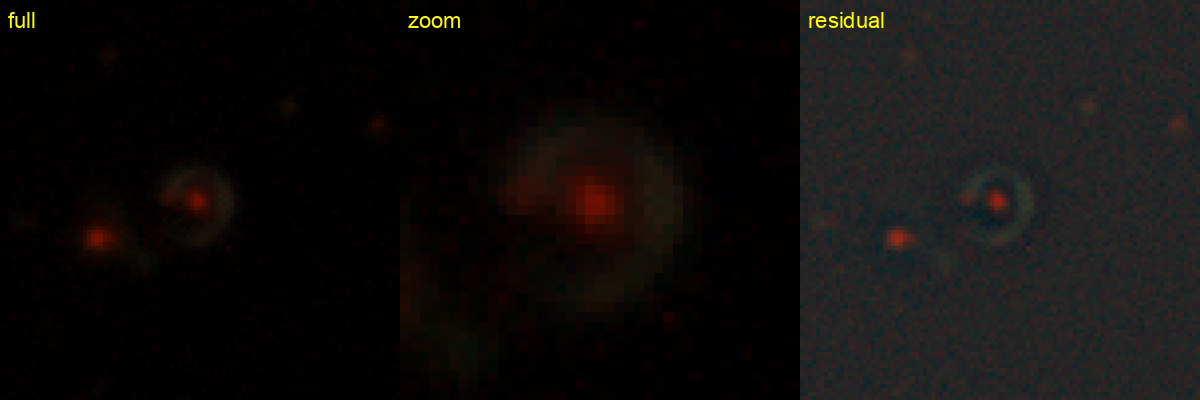
\includegraphics[width=\linewidth]{figures/res_s_98012_247.png}
\caption{\textbf{\#5}~\texttt{s\_98012\_247} --- RA 56.1462, Dec -44.7956; grade \textbf{A}, tier-1 $p_{\rm lens}$ 0.84, \vb{} 0.86. \textcolor{gray}{\textbf{KNOWN}} --- DES: \texttt{DES J034435.09-444743.9}, $0.18\arcsec$ (SIMBAD).}
\end{figure}
\begin{figure}[H]\centering
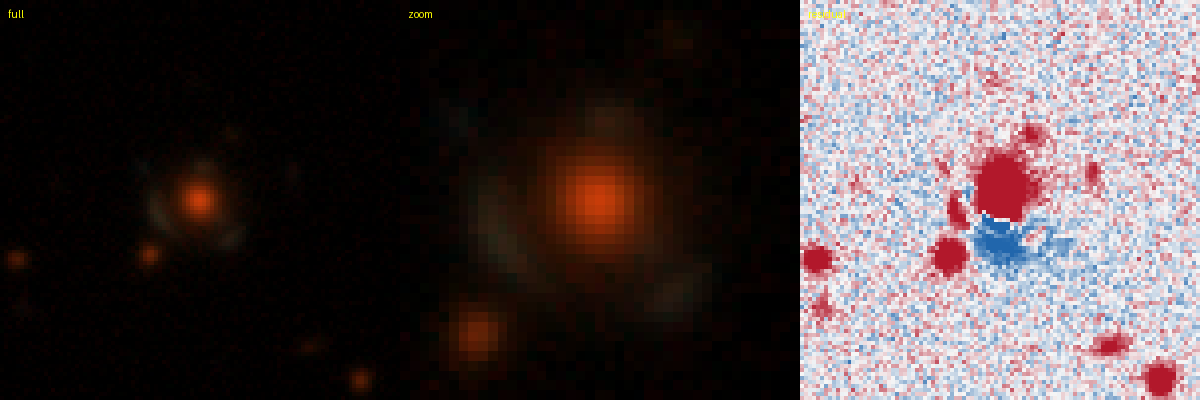
\includegraphics[width=\linewidth]{figures/res_s_124958_7349.png}
\caption{\textbf{\#6}~\texttt{s\_124958\_7349} --- RA 58.1768, Dec -38.4292; grade \textbf{A}, tier-1 $p_{\rm lens}$ 0.81, \vb{} 0.89. \textcolor{gray}{\textbf{KNOWN}} --- DES: \texttt{DES J035242.40-382544.9}, $0.01\arcsec$ (lineage).}
\end{figure}
\begin{figure}[H]\centering
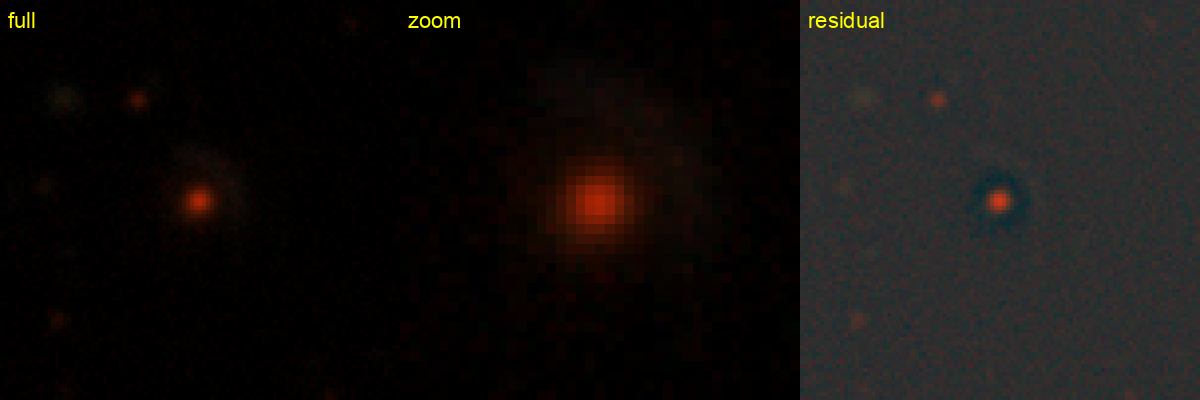
\includegraphics[width=\linewidth]{figures/res_s_191004_9637.png}
\caption{\textbf{\#7}~\texttt{s\_191004\_9637} --- RA 56.9356, Dec -24.9088; grade \textbf{A}, tier-1 $p_{\rm lens}$ 0.80, \vb{} 0.88. \textcolor{gray}{\textbf{KNOWN}} --- DES: \texttt{DES J034744.53-245431.4}, $0.20\arcsec$ (SIMBAD).}
\end{figure}
\begin{figure}[H]\centering
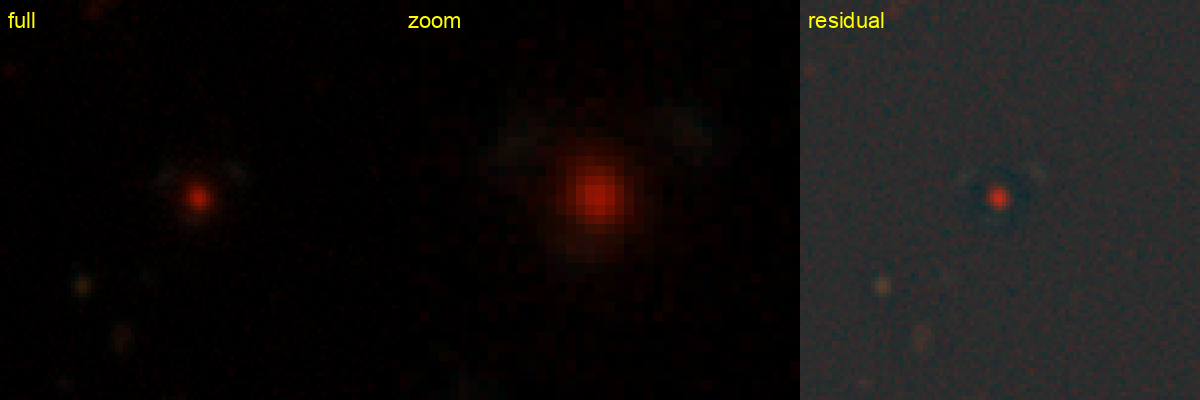
\includegraphics[width=\linewidth]{figures/res_s_80200_6872.png}
\caption{\textbf{\#8}~\texttt{s\_80200\_6872} --- RA 15.4919, Dec -49.2940; grade \textbf{A}, tier-1 $p_{\rm lens}$ 0.78, \vb{} 0.88. \textcolor{gray}{\textbf{KNOWN}} --- DES: \texttt{DES J010158.03-491738.1}, $0.12\arcsec$ (SIMBAD).}
\end{figure}
\begin{figure}[H]\centering
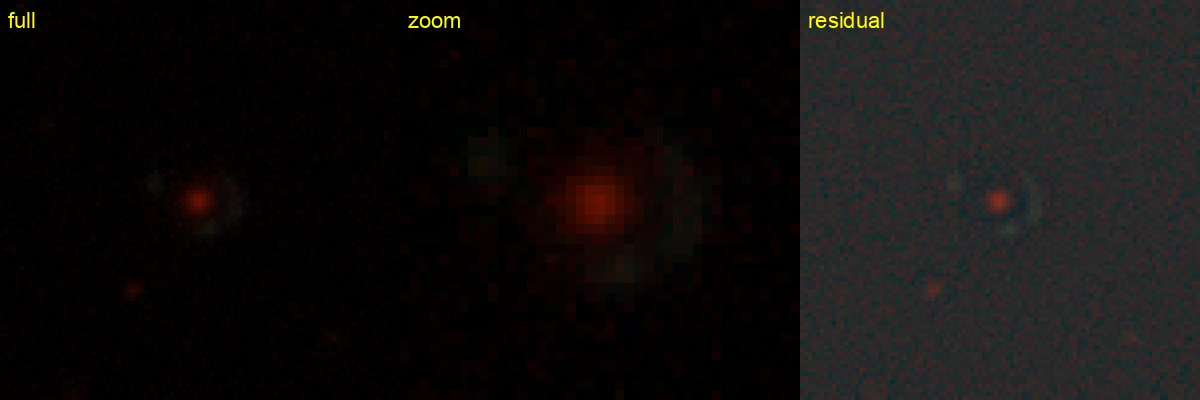
\includegraphics[width=\linewidth]{figures/res_s_180593_5604.png}
\caption{\textbf{\#10}~\texttt{s\_180593\_5604} --- RA 44.0974, Dec -27.1218; grade \textbf{B}, tier-1 $p_{\rm lens}$ 0.63, \vb{} 0.88. \textcolor{gray}{\textbf{KNOWN}} --- DES: \texttt{DES J025623.36-270718.5}, $0.28\arcsec$ (SIMBAD).}
\end{figure}
\begin{figure}[H]\centering
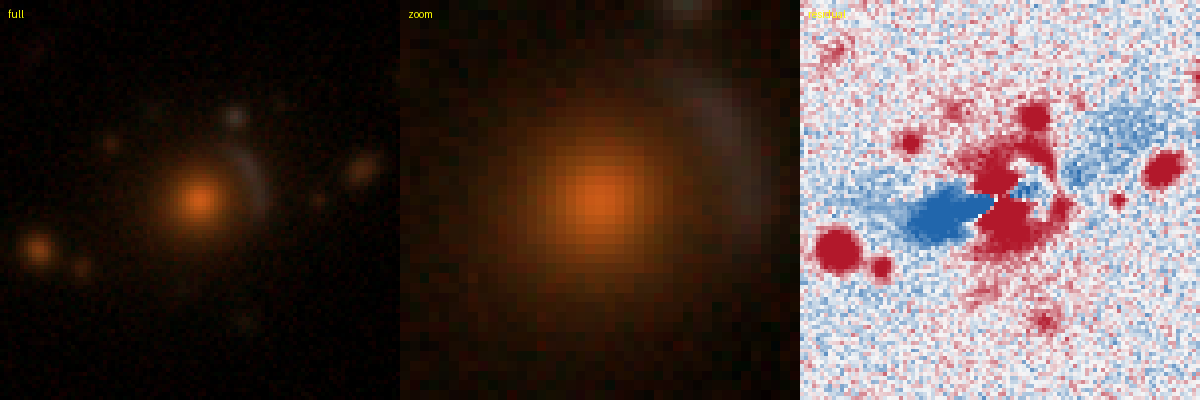
\includegraphics[width=\linewidth]{figures/res_s_292418_3907.png}
\caption{\textbf{\#11}~\texttt{s\_292418\_3907} --- RA 216.8280, Dec -6.7541; grade \textbf{B}, tier-1 $p_{\rm lens}$ 0.62, \vb{} 0.89. \textcolor{gray}{\textbf{KNOWN}} --- Huang+2020: \texttt{DESI-216.8280-06.7541}, $0.15\arcsec$ (lineage).}
\end{figure}
\begin{figure}[H]\centering
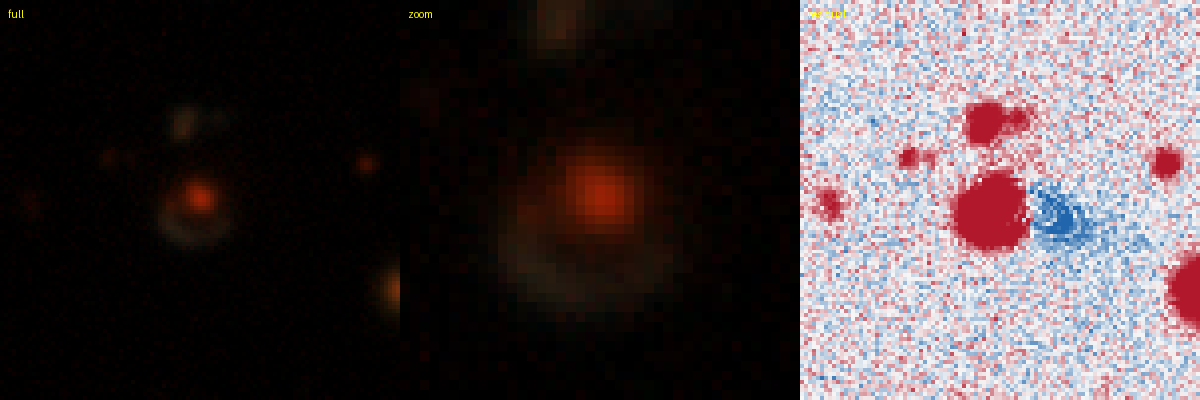
\includegraphics[width=\linewidth]{figures/res_s_232538_8716.png}
\caption{\textbf{\#12}~\texttt{s\_232538\_8716} --- RA 25.2755, Dec -17.2232; grade \textbf{B}, tier-1 $p_{\rm lens}$ 0.62, \vb{} 0.85. \textcolor{gray}{\textbf{KNOWN}} --- Huang+2020: \texttt{DESI-025.2755-17.2232}, $0.19\arcsec$ (lineage).}
\end{figure}
\begin{figure}[H]\centering
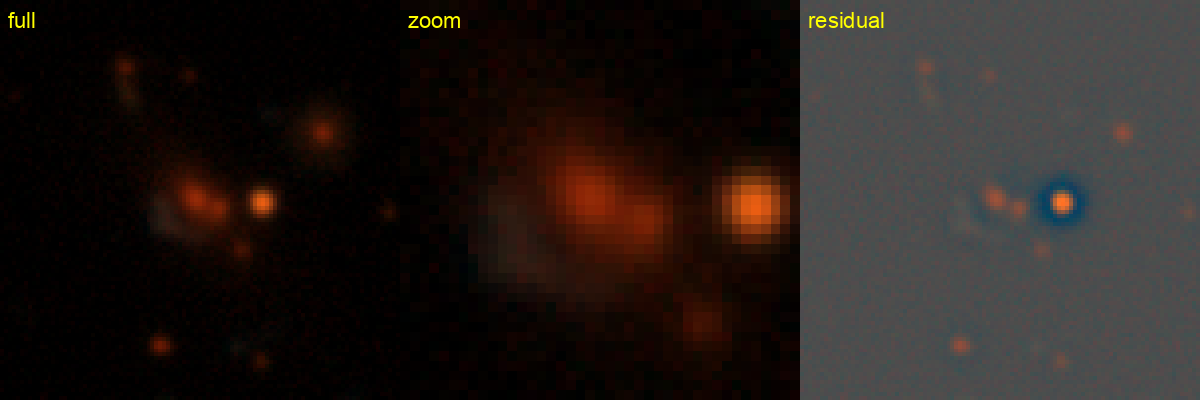
\includegraphics[width=\linewidth]{figures/res_s_42996_3467.png}
\caption{\textbf{\#14}~\texttt{s\_42996\_3467} --- RA 53.7444, Dec -60.5805; grade \textbf{B}, tier-1 $p_{\rm lens}$ 0.60, \vb{} 0.90. \textcolor{gray}{\textbf{KNOWN}} --- DES: \texttt{DES J033458.64-603450.0}, $0.15\arcsec$ (SIMBAD).}
\end{figure}
\begin{figure}[H]\centering
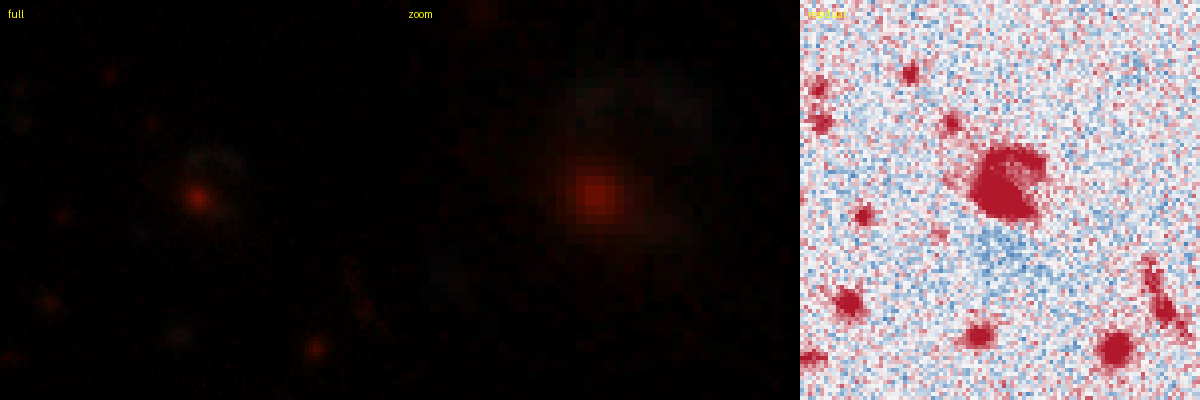
\includegraphics[width=\linewidth]{figures/res_s_188493_9685.png}
\caption{\textbf{\#16}~\texttt{s\_188493\_9685} --- RA 83.4556, Dec -25.6151; grade \textbf{B}, tier-1 $p_{\rm lens}$ 0.60, \vb{} 0.88. \textcolor{gray}{\textbf{KNOWN}} --- DES: \texttt{DES J053349.32-253654.3}, $0.15\arcsec$ (SIMBAD).}
\end{figure}
\begin{figure}[H]\centering
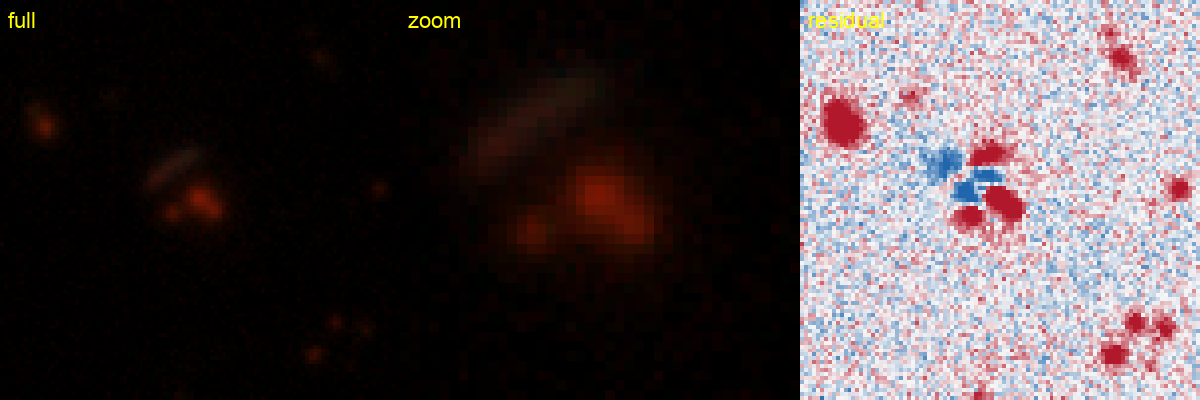
\includegraphics[width=\linewidth]{figures/res_s_38835_314.png}
\caption{\textbf{\#17}~\texttt{s\_38835\_314} --- RA 56.6543, Dec -61.9792; grade \textbf{B}, tier-1 $p_{\rm lens}$ 0.60, \vb{} 0.84. \textcolor{gray}{\textbf{KNOWN}} --- DES: \texttt{[DBL2017] DES J0346-6158 (A)}, $0.23\arcsec$ (SIMBAD).}
\end{figure}
\begin{figure}[H]\centering
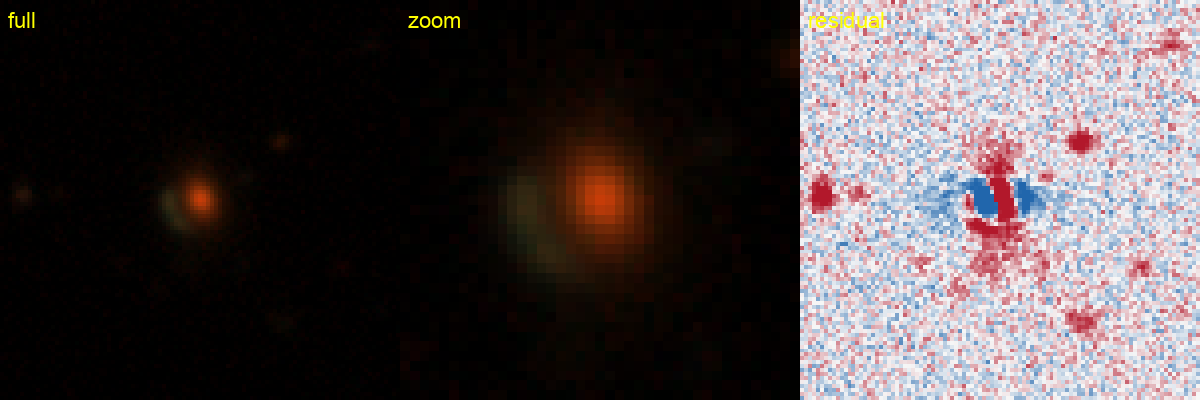
\includegraphics[width=\linewidth]{figures/res_s_240846_8850.png}
\caption{\textbf{\#19}~\texttt{s\_240846\_8850} --- RA 30.2832, Dec -15.8547; grade \textbf{B}, tier-1 $p_{\rm lens}$ 0.60, \vb{} 0.80. \textcolor{gray}{\textbf{KNOWN}} --- Huang+2020: \texttt{DESI-030.2832-15.8547}, $0.15\arcsec$ (lineage).}
\end{figure}
\begin{figure}[H]\centering
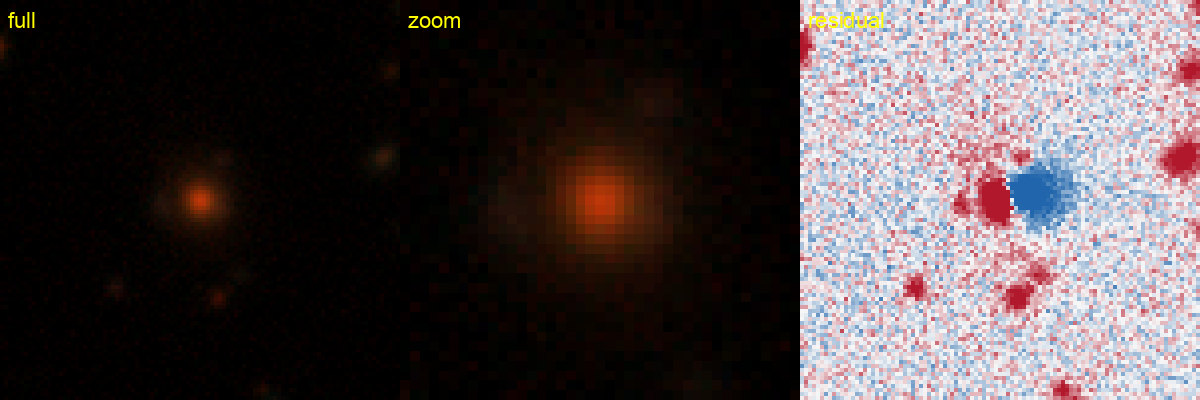
\includegraphics[width=\linewidth]{figures/res_s_111542_5062.png}
\caption{\textbf{\#20}~\texttt{s\_111542\_5062} --- RA 4.8181, Dec -41.6141; grade \textbf{B}, tier-1 $p_{\rm lens}$ 0.60, \vb{} 0.77. \textcolor{gray}{\textbf{KNOWN}} --- DES: \texttt{DES J001916.32-413650.5}, $0.22\arcsec$ (SIMBAD).}
\end{figure}
\begin{figure}[H]\centering
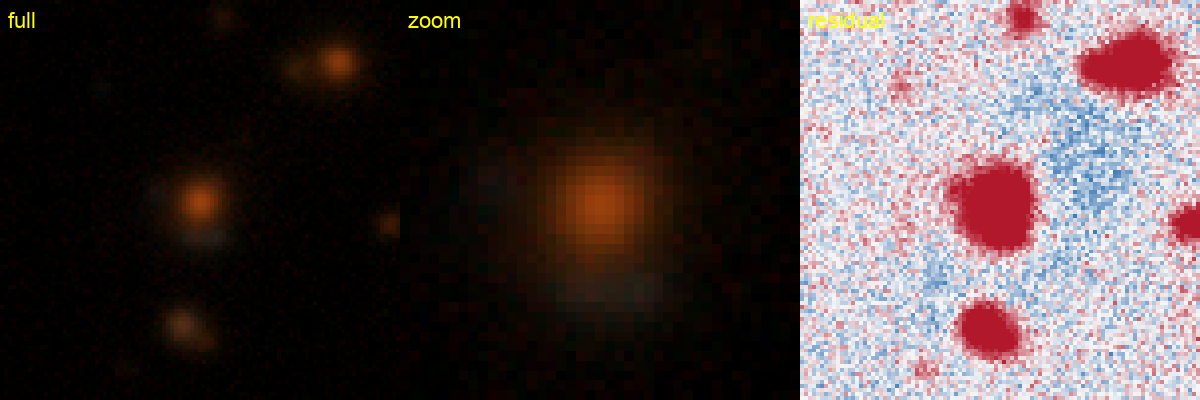
\includegraphics[width=\linewidth]{figures/res_s_290988_3355.png}
\caption{\textbf{\#21}~\texttt{s\_290988\_3355} --- RA 217.1429, Dec -7.0963; grade \textbf{B}, tier-1 $p_{\rm lens}$ 0.58, \vb{} 0.75. \textcolor{gray}{\textbf{KNOWN}} --- Huang+2020: \texttt{DESI-217.1429-07.0963}, $0.15\arcsec$ (lineage).}
\end{figure}
\begin{figure}[H]\centering
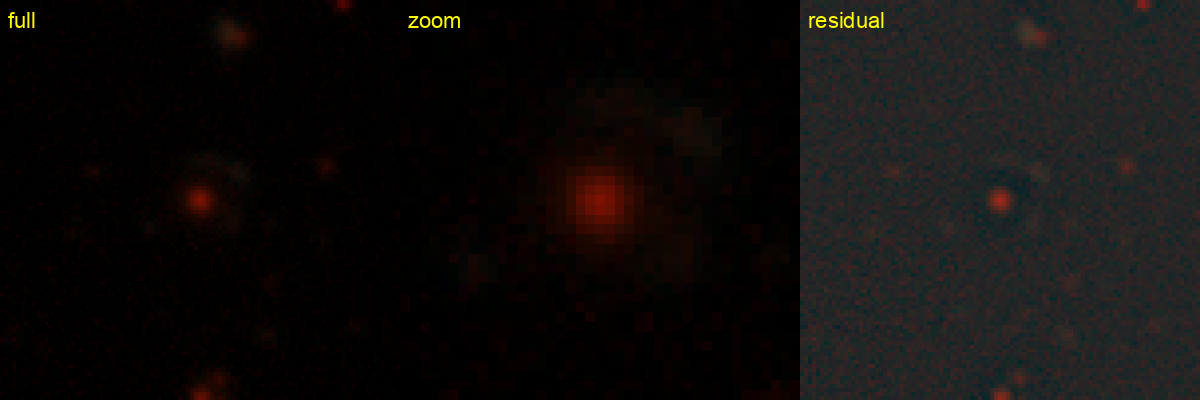
\includegraphics[width=\linewidth]{figures/res_s_50907_11900.png}
\caption{\textbf{\#23}~\texttt{s\_50907\_11900} --- RA 303.5808, Dec -57.9504; grade \textbf{B}, tier-1 $p_{\rm lens}$ 0.58, \vb{} 0.74. \textcolor{gray}{\textbf{KNOWN}} --- DES: \texttt{DES J201419.38-575701.4}, $0.15\arcsec$ (SIMBAD).}
\end{figure}
\begin{figure}[H]\centering
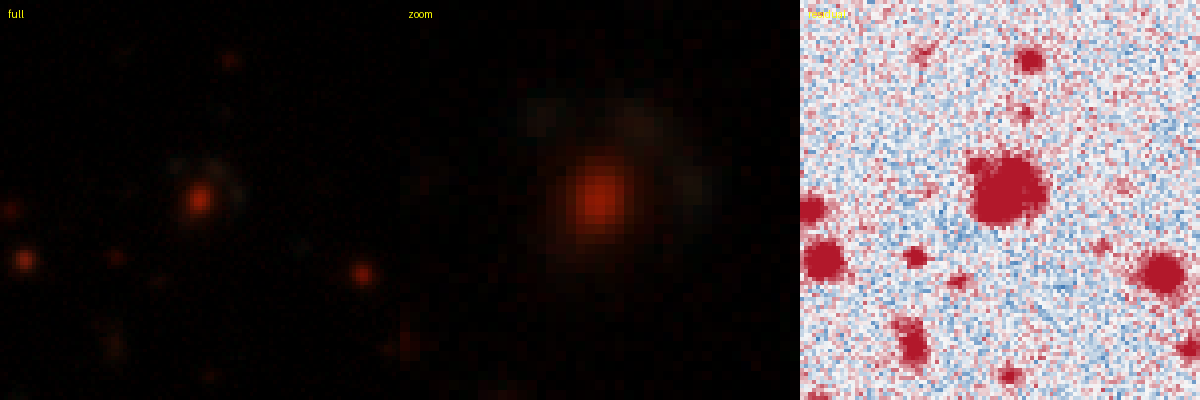
\includegraphics[width=\linewidth]{figures/res_s_34114_11363.png}
\caption{\textbf{\#24}~\texttt{s\_34114\_11363} --- RA 353.7468, Dec -64.0687; grade \textbf{B}, tier-1 $p_{\rm lens}$ 0.55, \vb{} 0.90. \textcolor{gray}{\textbf{KNOWN}} --- DES: \texttt{DES J233459.19-640406.9}, $0.32\arcsec$ (SIMBAD).}
\end{figure}
\begin{figure}[H]\centering
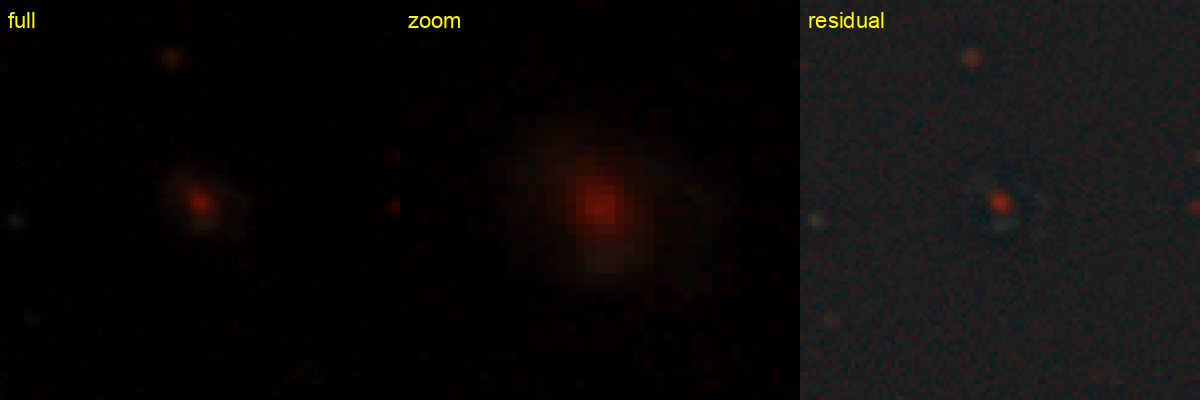
\includegraphics[width=\linewidth]{figures/res_s_61626_1035.png}
\caption{\textbf{\#25}~\texttt{s\_61626\_1035} --- RA 65.1782, Dec -54.3770; grade \textbf{B}, tier-1 $p_{\rm lens}$ 0.55, \vb{} 0.87. \textcolor{gray}{\textbf{KNOWN}} --- DES: \texttt{DES J042042.76-542237.4}, $0.18\arcsec$ (SIMBAD).}
\end{figure}
\begin{figure}[H]\centering
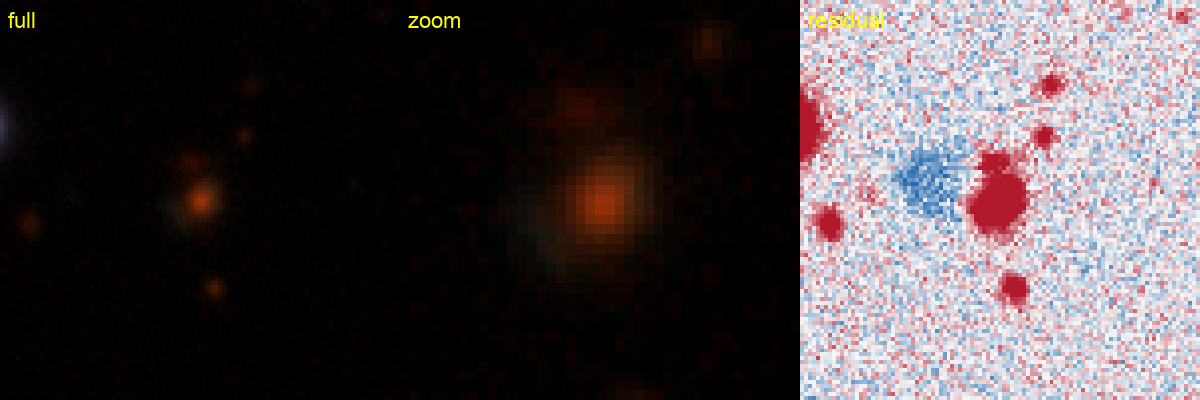
\includegraphics[width=\linewidth]{figures/res_s_159172_8702.png}
\caption{\textbf{\#26}~\texttt{s\_159172\_8702} --- RA 37.5699, Dec -31.3669; grade \textbf{B}, tier-1 $p_{\rm lens}$ 0.55, \vb{} 0.82. \textcolor{gray}{\textbf{KNOWN}} --- DES: \texttt{DES J023016.77-312200.8}, $0.07\arcsec$ (SIMBAD).}
\end{figure}
\begin{figure}[H]\centering
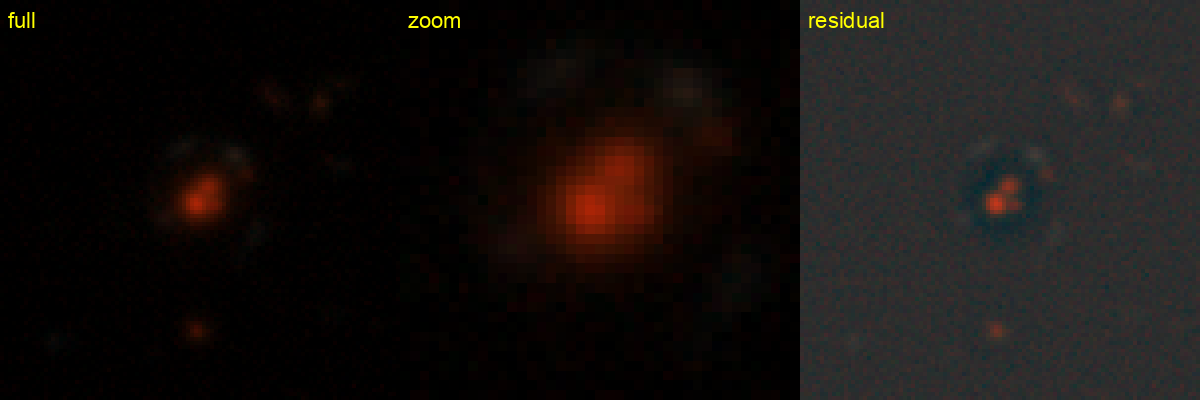
\includegraphics[width=\linewidth]{figures/res_s_197474_9756.png}
\caption{\textbf{\#27}~\texttt{s\_197474\_9756} --- RA 30.7668, Dec -23.6341; grade \textbf{B}, tier-1 $p_{\rm lens}$ 0.55, \vb{} 0.81. \textcolor{gray}{\textbf{KNOWN}} --- DES: \texttt{DES J020304.01-233802.5}, $0.22\arcsec$ (SIMBAD).}
\end{figure}
\begin{figure}[H]\centering
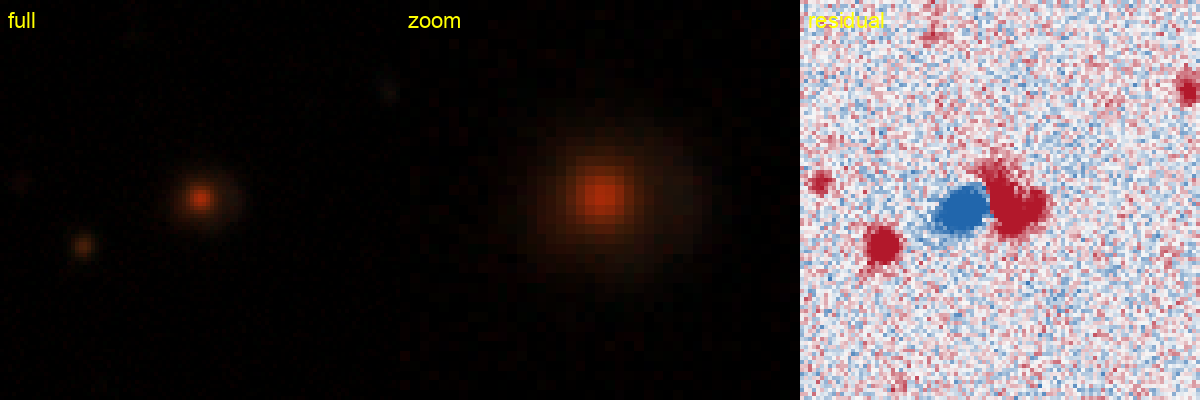
\includegraphics[width=\linewidth]{figures/res_s_310225_1602.png}
\caption{\textbf{\#29}~\texttt{s\_310225\_1602} --- RA 3.2923, Dec -3.5960; grade \textbf{B}, tier-1 $p_{\rm lens}$ 0.52, \vb{} 0.75. \textcolor{gray}{\textbf{KNOWN}} --- DES: \texttt{DES J001310.13-033545.4}, $0.18\arcsec$ (SIMBAD).}
\end{figure}
\begin{figure}[H]\centering
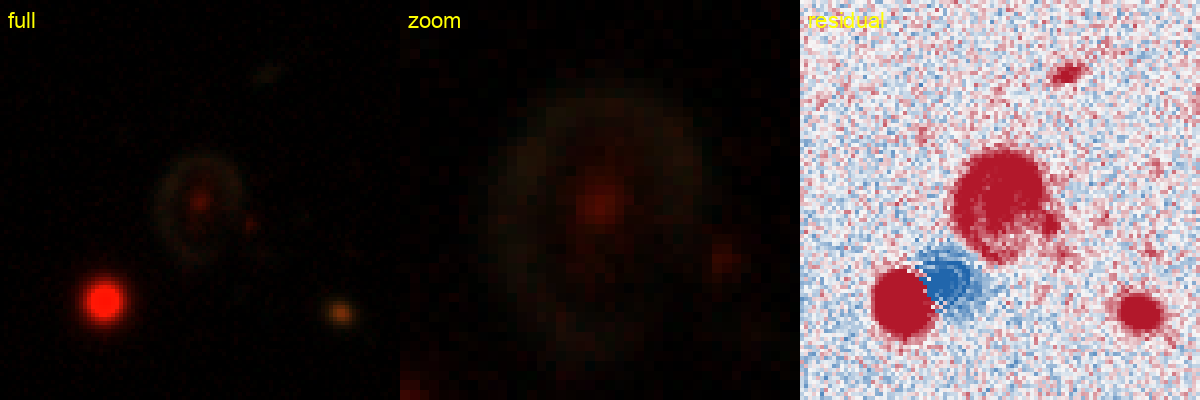
\includegraphics[width=\linewidth]{figures/res_s_61472_9399.png}
\caption{\textbf{\#30}~\texttt{s\_61472\_9399} --- RA 359.5200, Dec -54.6765; grade \textbf{B}, tier-1 $p_{\rm lens}$ 0.50, \vb{} 0.88. \textcolor{gray}{\textbf{KNOWN}} --- DES: \texttt{DES J235804.95-544034.4}, $1.73\arcsec$ (SIMBAD).}
\end{figure}
\begin{figure}[H]\centering
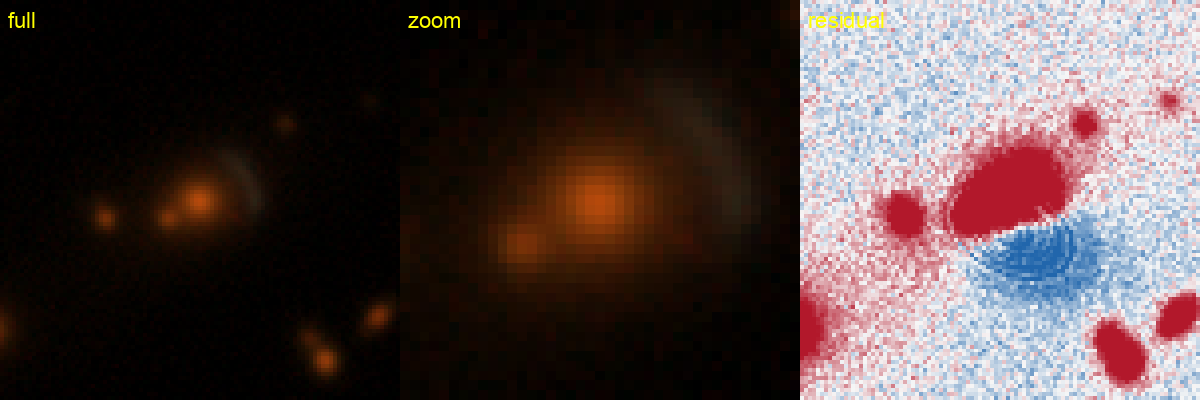
\includegraphics[width=\linewidth]{figures/res_s_137518_1133.png}
\caption{\textbf{\#31}~\texttt{s\_137518\_1133} --- RA 31.3588, Dec -35.6632; grade \textbf{B}, tier-1 $p_{\rm lens}$ 0.50, \vb{} 0.84. \textcolor{gray}{\textbf{KNOWN}} --- DES: \texttt{DES J020526.09-353947.4}, $0.14\arcsec$ (SIMBAD).}
\end{figure}
\begin{figure}[H]\centering
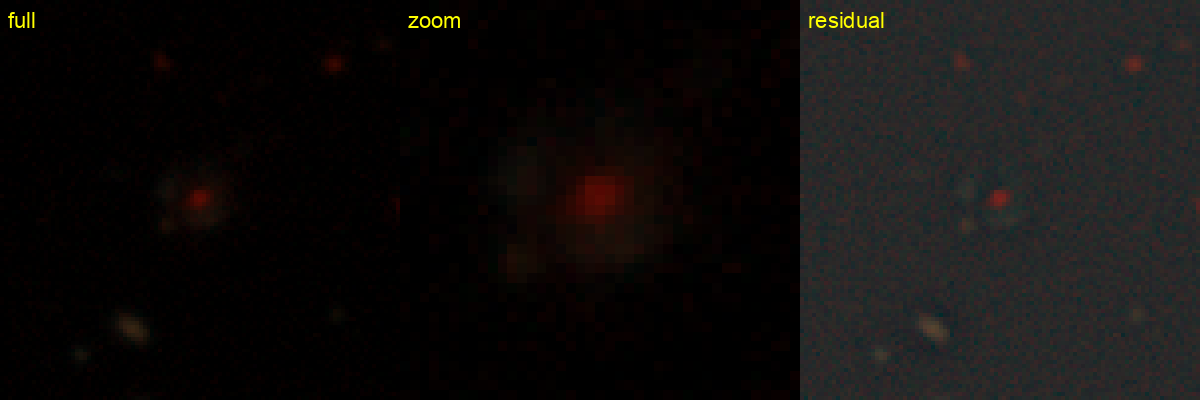
\includegraphics[width=\linewidth]{figures/res_s_43736_6056.png}
\caption{\textbf{\#33}~\texttt{s\_43736\_6056} --- RA 67.3945, Dec -60.1905; grade \textbf{B}, tier-1 $p_{\rm lens}$ 0.50, \vb{} 0.83. \textcolor{gray}{\textbf{KNOWN}} --- DES: \texttt{DES J042934.66-601126.3}, $0.35\arcsec$ (SIMBAD).}
\end{figure}
\begin{figure}[H]\centering
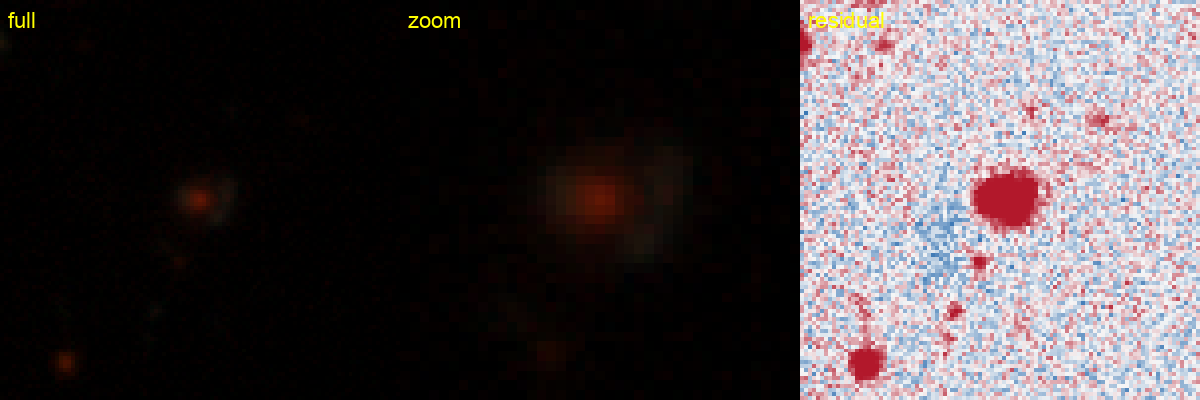
\includegraphics[width=\linewidth]{figures/res_s_257579_1725.png}
\caption{\textbf{\#34}~\texttt{s\_257579\_1725} --- RA 23.3422, Dec -12.8670; grade \textbf{B}, tier-1 $p_{\rm lens}$ 0.50, \vb{} 0.82. \textcolor{gray}{\textbf{KNOWN}} --- DES: \texttt{DES J013322.10-125201.2}, $0.27\arcsec$ (SIMBAD).}
\end{figure}
\begin{figure}[H]\centering
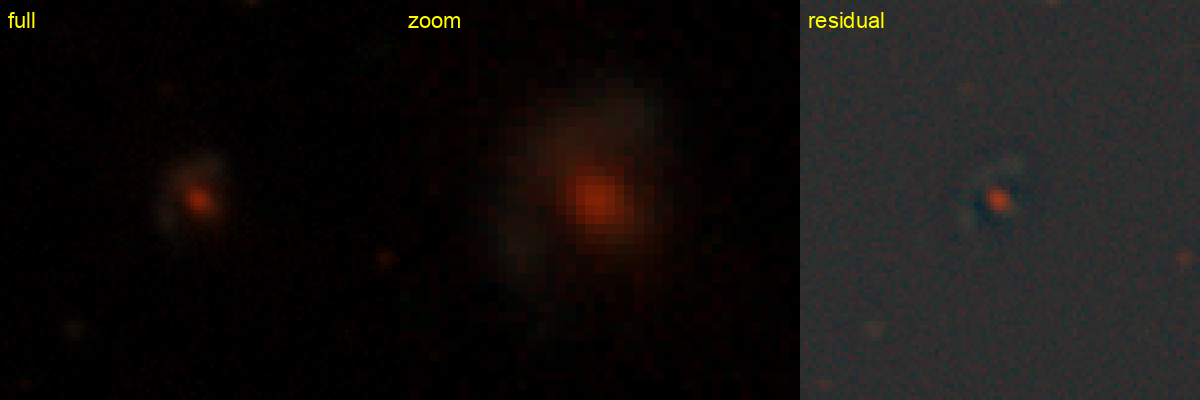
\includegraphics[width=\linewidth]{figures/res_s_301694_7426.png}
\caption{\textbf{\#37}~\texttt{s\_301694\_7426} --- RA 26.2679, Dec -4.9310; grade \textbf{B}, tier-1 $p_{\rm lens}$ 0.48, \vb{} 0.85. \textcolor{gray}{\textbf{KNOWN}} --- Huang+2020: \texttt{DESI-026.2679-04.9310}, $0.13\arcsec$ (lineage).}
\end{figure}
\begin{figure}[H]\centering
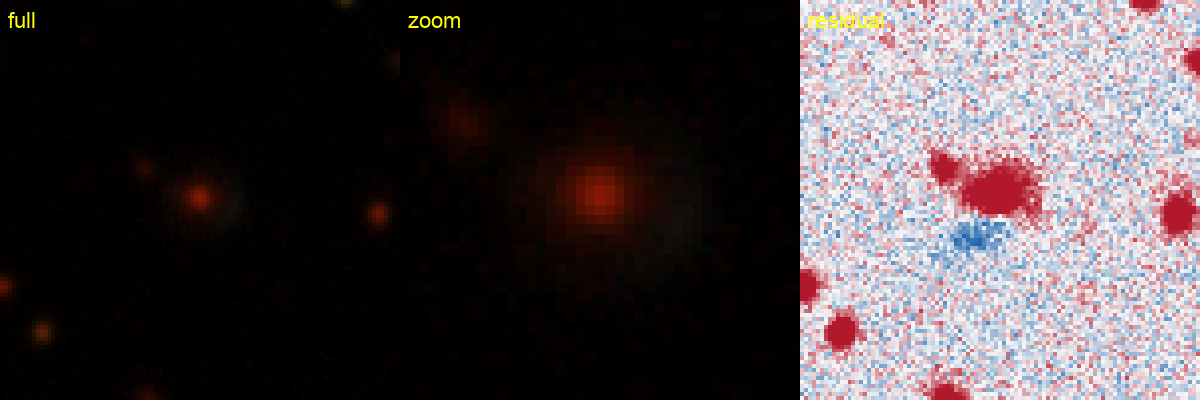
\includegraphics[width=\linewidth]{figures/res_s_58263_3751.png}
\caption{\textbf{\#38}~\texttt{s\_58263\_3751} --- RA 42.7179, Dec -55.4032; grade \textbf{B}, tier-1 $p_{\rm lens}$ 0.45, \vb{} 0.88. \textcolor{gray}{\textbf{KNOWN}} --- DES: \texttt{DES J025052.27-552411.7}, $0.22\arcsec$ (SIMBAD).}
\end{figure}
\begin{figure}[H]\centering
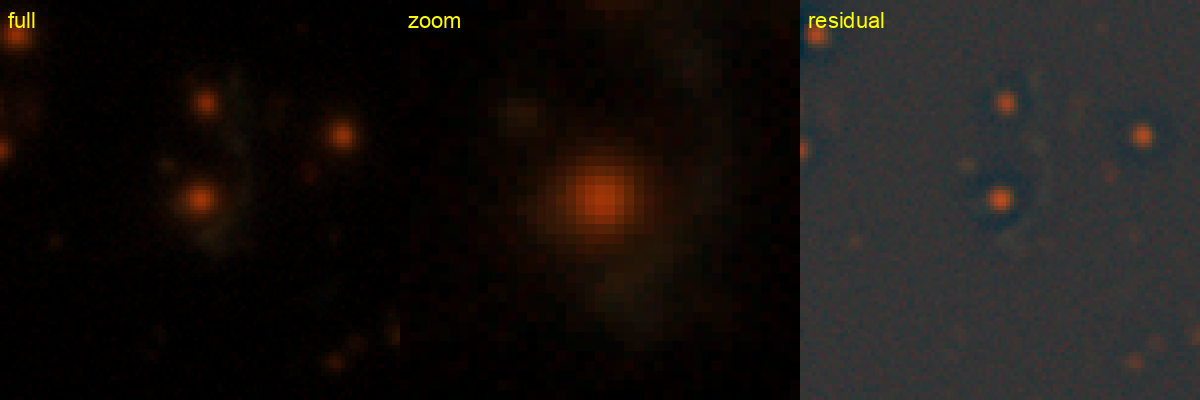
\includegraphics[width=\linewidth]{figures/res_s_194944_4494.png}
\caption{\textbf{\#39}~\texttt{s\_194944\_4494} --- RA 59.2045, Dec -24.1447; grade \textbf{B}, tier-1 $p_{\rm lens}$ 0.45, \vb{} 0.85. \textcolor{gray}{\textbf{KNOWN}} --- DES: \texttt{DES J035649.05-240841.1}, $0.28\arcsec$ (SIMBAD).}
\end{figure}
\begin{figure}[H]\centering
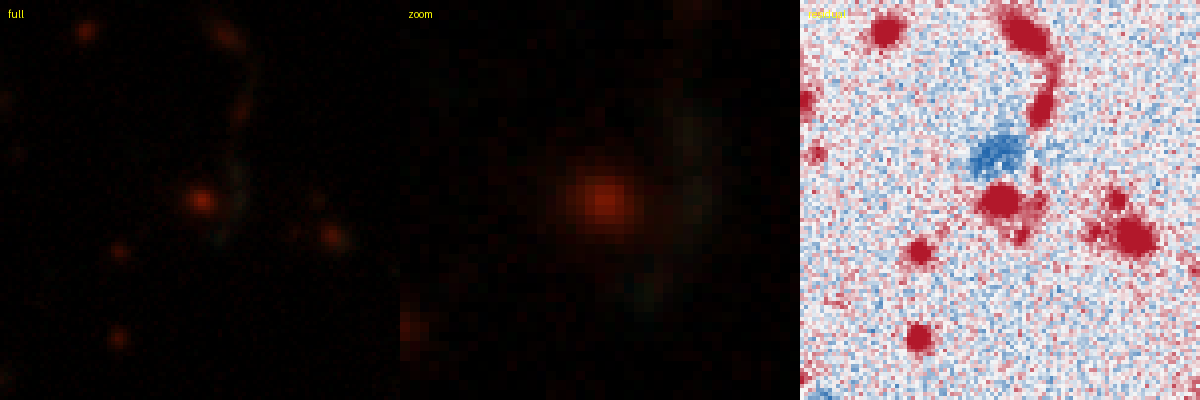
\includegraphics[width=\linewidth]{figures/res_s_280236_3353.png}
\caption{\textbf{\#40}~\texttt{s\_280236\_3353} --- RA 25.8623, Dec -8.8393; grade \textbf{B}, tier-1 $p_{\rm lens}$ 0.45, \vb{} 0.84. \textcolor{gray}{\textbf{KNOWN}} --- AGEL: \texttt{AGEL J014327-085021 system}, $0.93\arcsec$ (SIMBAD).}
\end{figure}
\begin{figure}[H]\centering
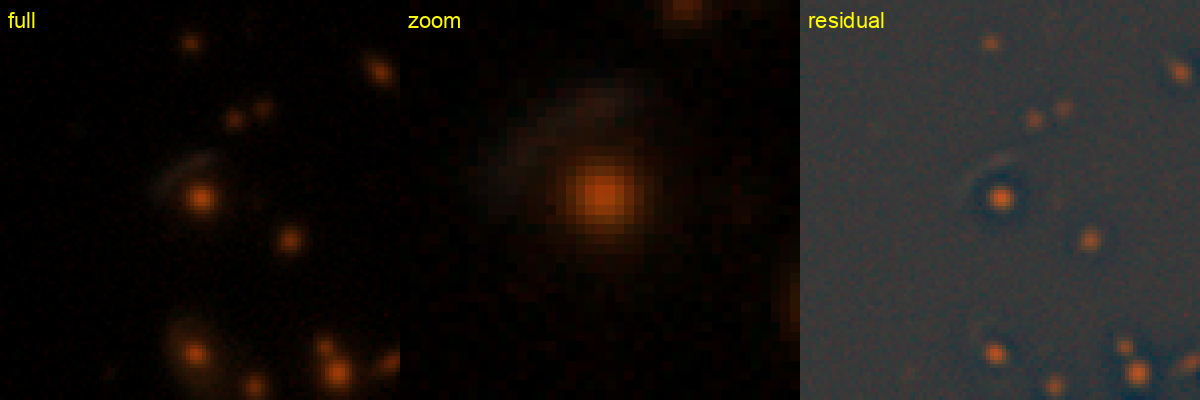
\includegraphics[width=\linewidth]{figures/res_s_82090_1248.png}
\caption{\textbf{\#42}~\texttt{s\_82090\_1248} --- RA 14.4037, Dec -48.8040; grade \textbf{B}, tier-1 $p_{\rm lens}$ 0.45, \vb{} 0.81. \textcolor{gray}{\textbf{KNOWN}} --- DES: \texttt{[DBL2017] DES J0057-4848 (A)}, $0.19\arcsec$ (SIMBAD).}
\end{figure}
\begin{figure}[H]\centering
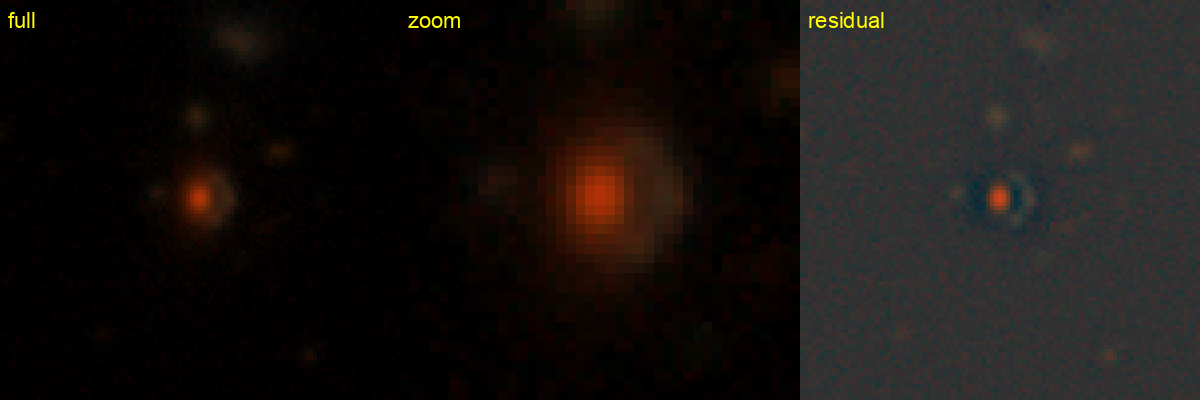
\includegraphics[width=\linewidth]{figures/res_s_156771_3446.png}
\caption{\textbf{\#47}~\texttt{s\_156771\_3446} --- RA 54.3219, Dec -31.8704; grade \textbf{B}, tier-1 $p_{\rm lens}$ 0.42, \vb{} 0.89. \textcolor{gray}{\textbf{KNOWN}} --- AGEL: \texttt{AGEL J033717-315214 system}, $0.99\arcsec$ (SIMBAD).}
\end{figure}
\begin{figure}[H]\centering
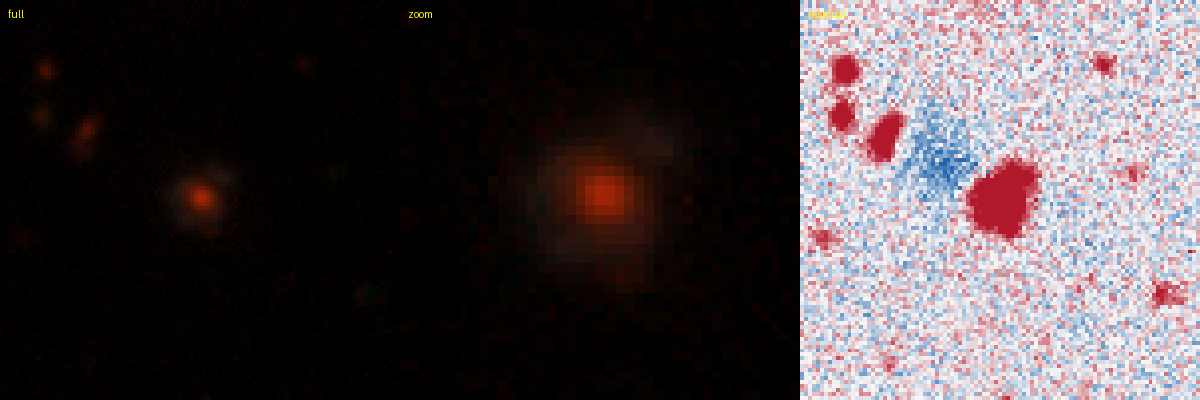
\includegraphics[width=\linewidth]{figures/res_s_94861_9433.png}
\caption{\textbf{\#48}~\texttt{s\_94861\_9433} --- RA 21.9716, Dec -45.5428; grade \textbf{B}, tier-1 $p_{\rm lens}$ 0.42, \vb{} 0.87. \textcolor{gray}{\textbf{KNOWN}} --- DES: \texttt{DES J012753.17-453233.8}, $0.17\arcsec$ (SIMBAD).}
\end{figure}
\begin{figure}[H]\centering
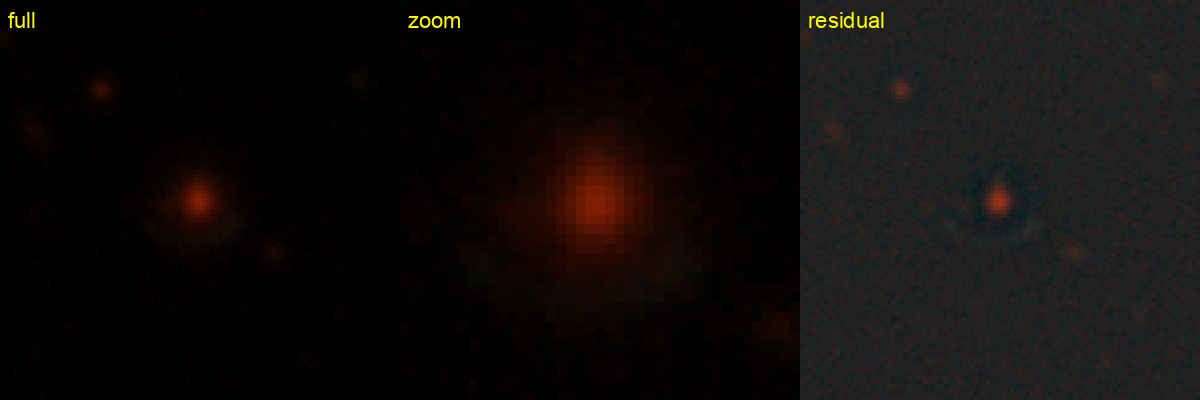
\includegraphics[width=\linewidth]{figures/res_s_102952_10164.png}
\caption{\textbf{\#49}~\texttt{s\_102952\_10164} --- RA 334.8017, Dec -43.8098; grade \textbf{B}, tier-1 $p_{\rm lens}$ 0.42, \vb{} 0.85. \textcolor{gray}{\textbf{KNOWN}} --- DES: \texttt{DES J221912.39-434835.1}, $0.01\arcsec$ (lineage).}
\end{figure}
\begin{figure}[H]\centering
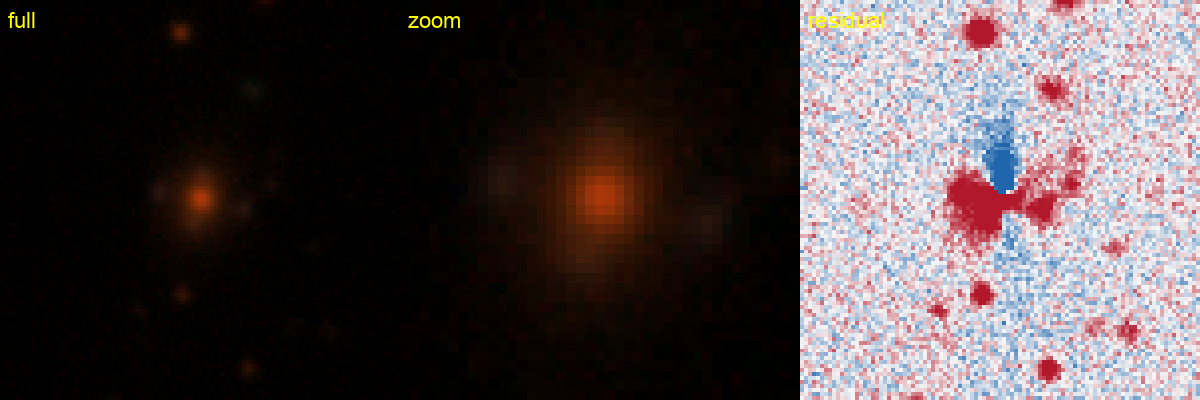
\includegraphics[width=\linewidth]{figures/res_s_90804_9850.png}
\caption{\textbf{\#50}~\texttt{s\_90804\_9850} --- RA 3.9284, Dec -46.6031; grade \textbf{B}, tier-1 $p_{\rm lens}$ 0.42, \vb{} 0.84. \textcolor{gray}{\textbf{KNOWN}} --- DES: \texttt{DES J001542.79-463610.9}, $0.16\arcsec$ (SIMBAD).}
\end{figure}
\begin{figure}[H]\centering
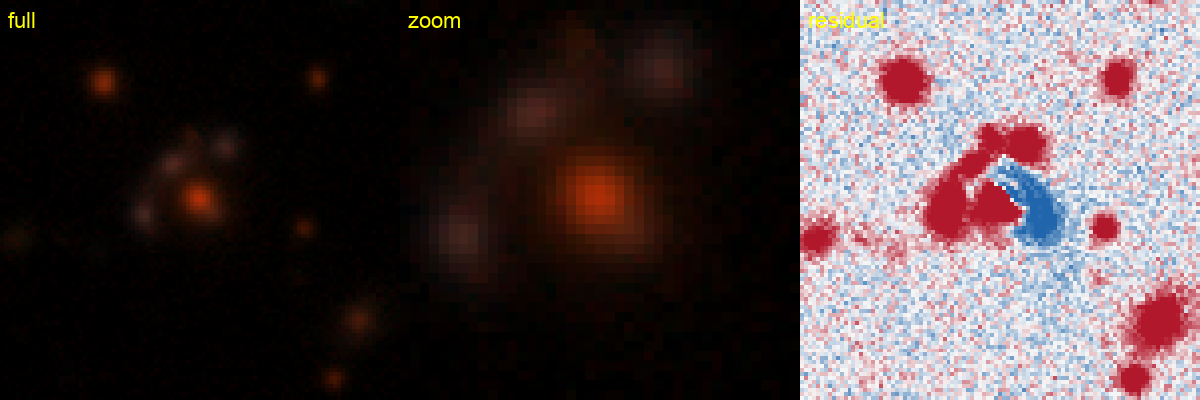
\includegraphics[width=\linewidth]{figures/res_s_71042_1653.png}
\caption{\textbf{\#51}~\texttt{s\_71042\_1653} --- RA 20.1760, Dec -51.7314; grade \textbf{B}, tier-1 $p_{\rm lens}$ 0.42, \vb{} 0.82. \textcolor{gray}{\textbf{KNOWN}} --- DES: \texttt{[DBL2017] DES J0120-5143 (A)}, $0.19\arcsec$ (SIMBAD).}
\end{figure}
\begin{figure}[H]\centering
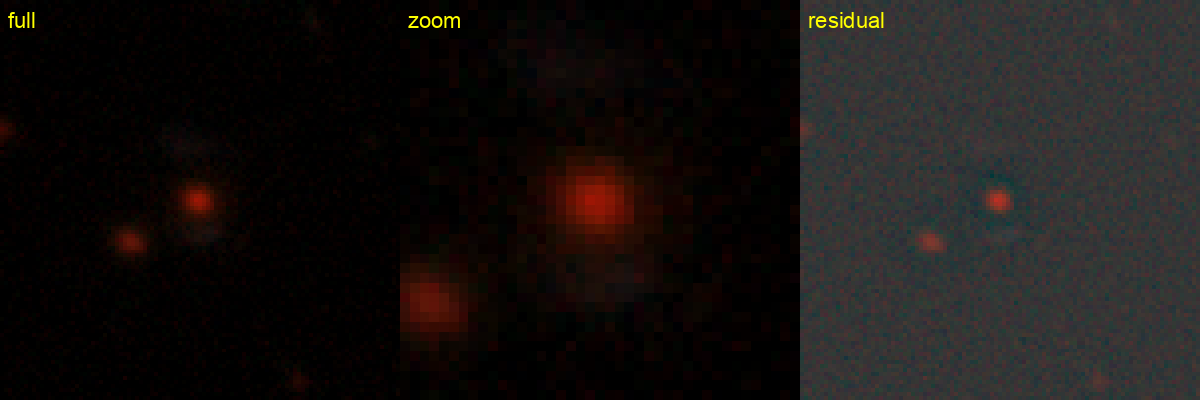
\includegraphics[width=\linewidth]{figures/res_s_381188_1199.png}
\caption{\textbf{\#54}~\texttt{s\_381188\_1199} --- RA 144.1511, Dec +8.8633; grade \textbf{B}, tier-1 $p_{\rm lens}$ 0.40, \vb{} 0.90. \textcolor{gray}{\textbf{KNOWN}} --- Huang+2020: \texttt{DESI-144.1511+08.8633}, $0.20\arcsec$ (lineage).}
\end{figure}
\begin{figure}[H]\centering
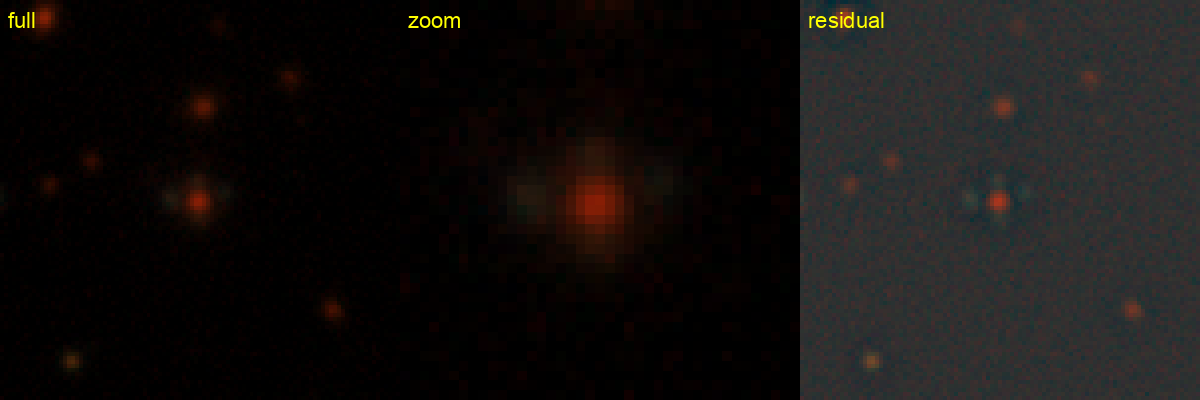
\includegraphics[width=\linewidth]{figures/res_s_235296_3732.png}
\caption{\textbf{\#55}~\texttt{s\_235296\_3732} --- RA 25.6457, Dec -16.8049; grade \textbf{B}, tier-1 $p_{\rm lens}$ 0.40, \vb{} 0.88. \textcolor{gray}{\textbf{KNOWN}} --- AGEL: \texttt{AGEL J014235-164818 system}, $0.86\arcsec$ (SIMBAD).}
\end{figure}
\begin{figure}[H]\centering
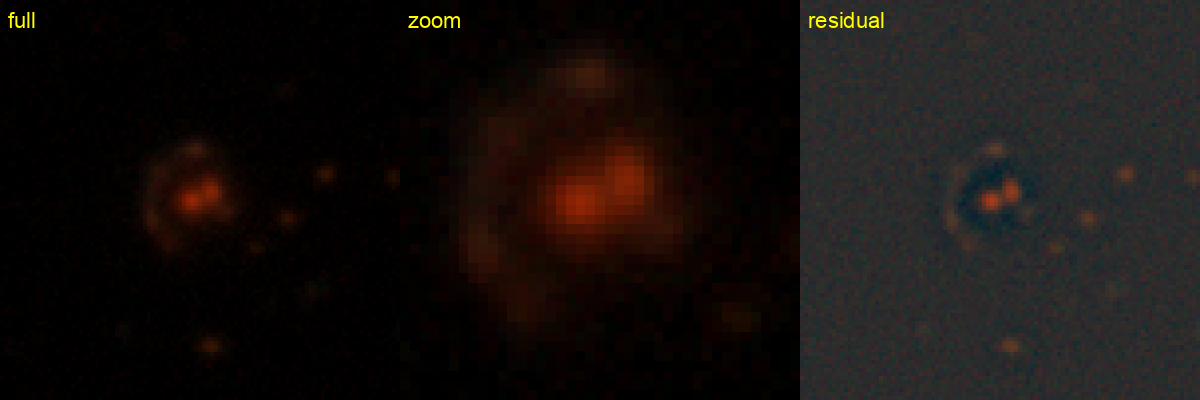
\includegraphics[width=\linewidth]{figures/res_s_91761_4679.png}
\caption{\textbf{\#57}~\texttt{s\_91761\_4679} --- RA 350.3683, Dec -46.5138; grade \textbf{B}, tier-1 $p_{\rm lens}$ 0.40, \vb{} 0.86. \textcolor{gray}{\textbf{KNOWN}} --- DES: \texttt{DES J232128.37-463049.3}, $0.25\arcsec$ (SIMBAD).}
\end{figure}
\begin{figure}[H]\centering
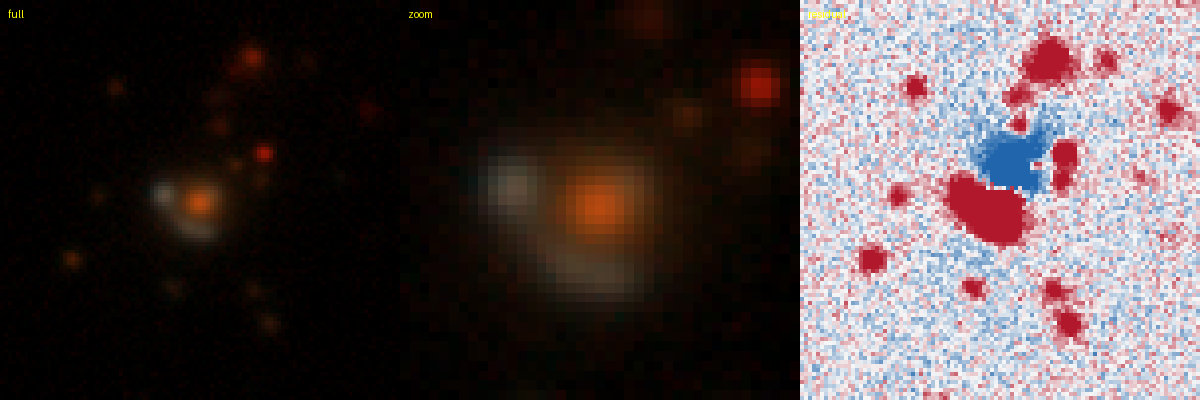
\includegraphics[width=\linewidth]{figures/res_s_107312_5223.png}
\caption{\textbf{\#59}~\texttt{s\_107312\_5223} --- RA 23.8451, Dec -42.5398; grade \textbf{B}, tier-1 $p_{\rm lens}$ 0.40, \vb{} 0.85. \textcolor{gray}{\textbf{KNOWN}} --- DES: \texttt{[DBL2017] DES J0135-4232 (A)}, $0.18\arcsec$ (SIMBAD).}
\end{figure}
\begin{figure}[H]\centering
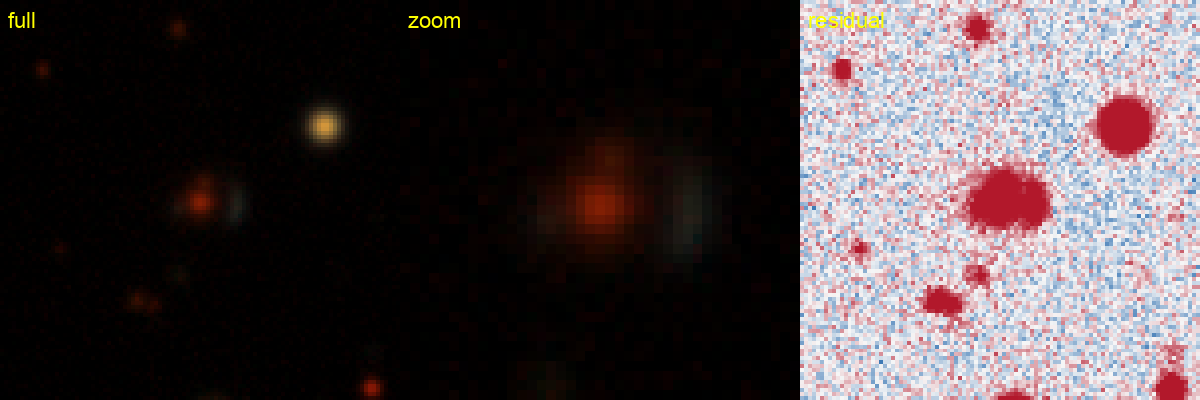
\includegraphics[width=\linewidth]{figures/res_s_69087_268.png}
\caption{\textbf{\#60}~\texttt{s\_69087\_268} --- RA 307.2325, Dec -52.5218; grade \textbf{B}, tier-1 $p_{\rm lens}$ 0.40, \vb{} 0.81. \textcolor{gray}{\textbf{KNOWN}} --- DES: \texttt{DES J202855.79-523118.3}, $0.12\arcsec$ (SIMBAD).}
\end{figure}
\begin{figure}[H]\centering
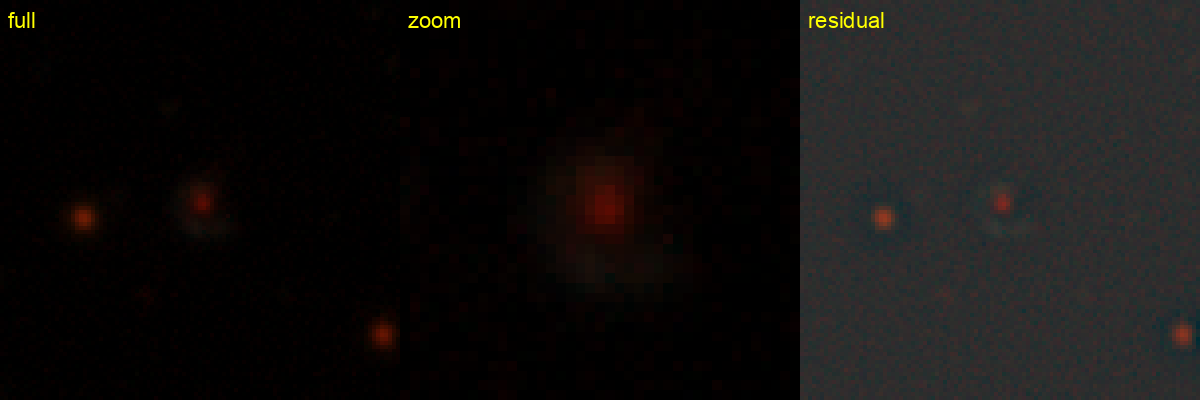
\includegraphics[width=\linewidth]{figures/res_s_165468_9648.png}
\caption{\textbf{\#61}~\texttt{s\_165468\_9648} --- RA 64.7771, Dec -29.9937; grade \textbf{B}, tier-1 $p_{\rm lens}$ 0.40, \vb{} 0.78. \textcolor{gray}{\textbf{KNOWN}} --- DES: \texttt{DES J041906.50-295937.7}, $0.49\arcsec$ (SIMBAD).}
\end{figure}
\begin{figure}[H]\centering
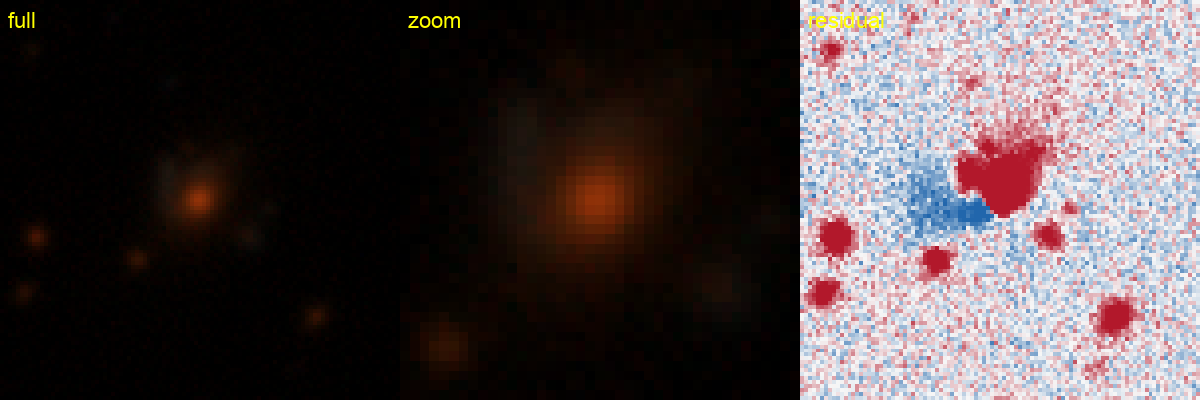
\includegraphics[width=\linewidth]{figures/res_s_256199_9097.png}
\caption{\textbf{\#62}~\texttt{s\_256199\_9097} --- RA 29.6819, Dec -13.0258; grade \textbf{B}, tier-1 $p_{\rm lens}$ 0.40, \vb{} 0.78. \textcolor{gray}{\textbf{KNOWN}} --- DES: \texttt{DES J015843.66-130132.8}, $0.18\arcsec$ (SIMBAD).}
\end{figure}
\begin{figure}[H]\centering
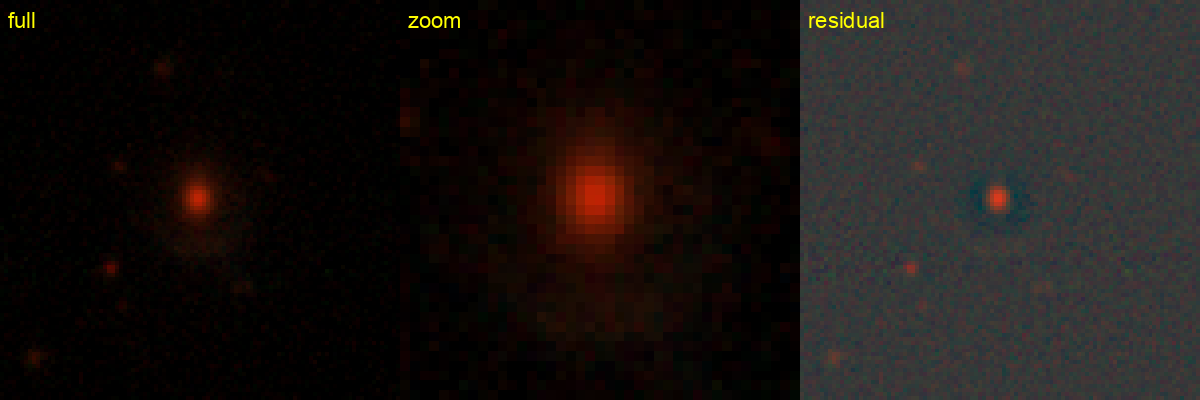
\includegraphics[width=\linewidth]{figures/res_s_364017_5199.png}
\caption{\textbf{\#63}~\texttt{s\_364017\_5199} --- RA 141.0626, Dec +5.7690; grade \textbf{B}, tier-1 $p_{\rm lens}$ 0.40, \vb{} 0.77. \textcolor{gray}{\textbf{KNOWN}} --- Huang+2020: \texttt{DESI-141.0626+05.7690}, $0.11\arcsec$ (lineage).}
\end{figure}
\begin{figure}[H]\centering
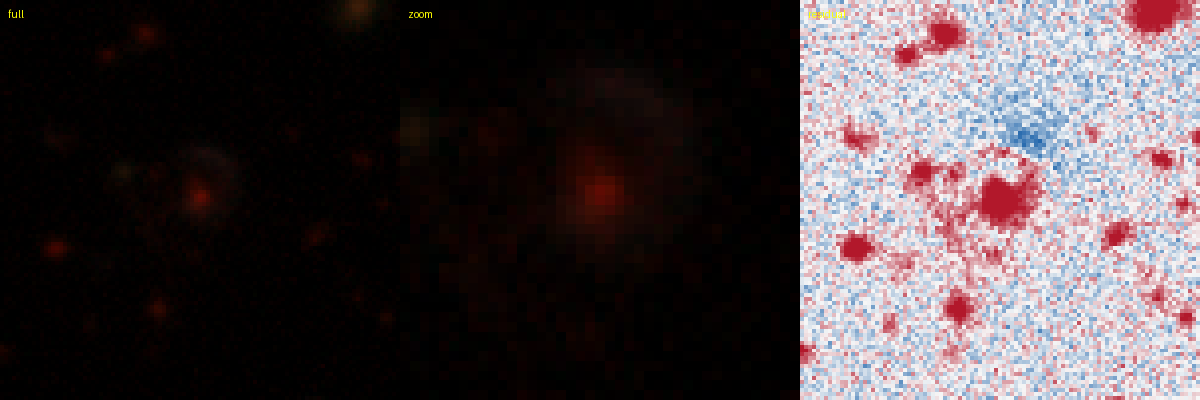
\includegraphics[width=\linewidth]{figures/res_s_119342_4136.png}
\caption{\textbf{\#66}~\texttt{s\_119342\_4136} --- RA 50.7164, Dec -39.7694; grade \textbf{B}, tier-1 $p_{\rm lens}$ 0.38, \vb{} 0.90. \textcolor{gray}{\textbf{KNOWN}} --- DES: \texttt{DES J032251.91-394609.6}, $0.17\arcsec$ (SIMBAD).}
\end{figure}
\begin{figure}[H]\centering
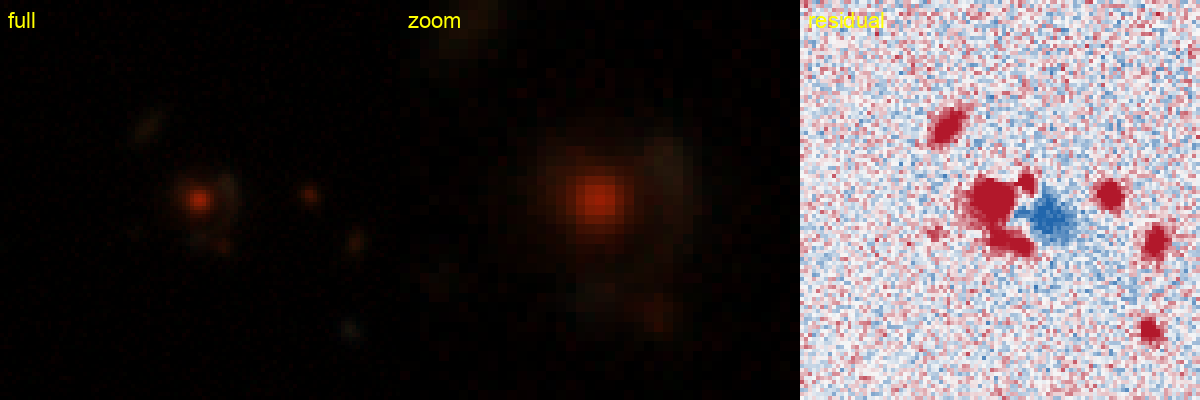
\includegraphics[width=\linewidth]{figures/res_s_209576_5226.png}
\caption{\textbf{\#68}~\texttt{s\_209576\_5226} --- RA 65.5760, Dec -21.5461; grade \textbf{B}, tier-1 $p_{\rm lens}$ 0.38, \vb{} 0.86. \textcolor{gray}{\textbf{KNOWN}} --- DES: \texttt{DES J042218.21-213245.8}, $0.28\arcsec$ (SIMBAD).}
\end{figure}
\begin{figure}[H]\centering
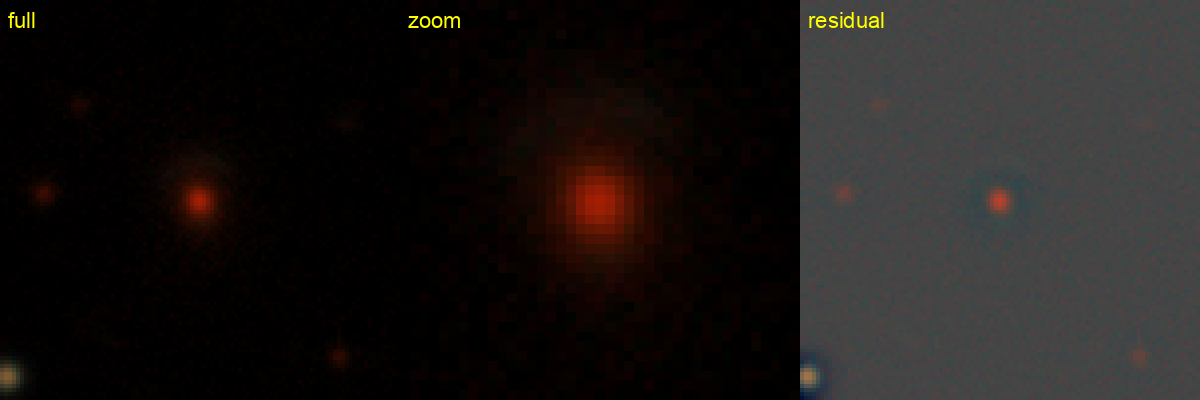
\includegraphics[width=\linewidth]{figures/res_s_225679_7025.png}
\caption{\textbf{\#69}~\texttt{s\_225679\_7025} --- RA 25.7203, Dec -18.5211; grade \textbf{B}, tier-1 $p_{\rm lens}$ 0.38, \vb{} 0.79. \textcolor{gray}{\textbf{KNOWN}} --- AGEL: \texttt{AGEL J014253-183116 system}, $0.94\arcsec$ (SIMBAD).}
\end{figure}
\begin{figure}[H]\centering
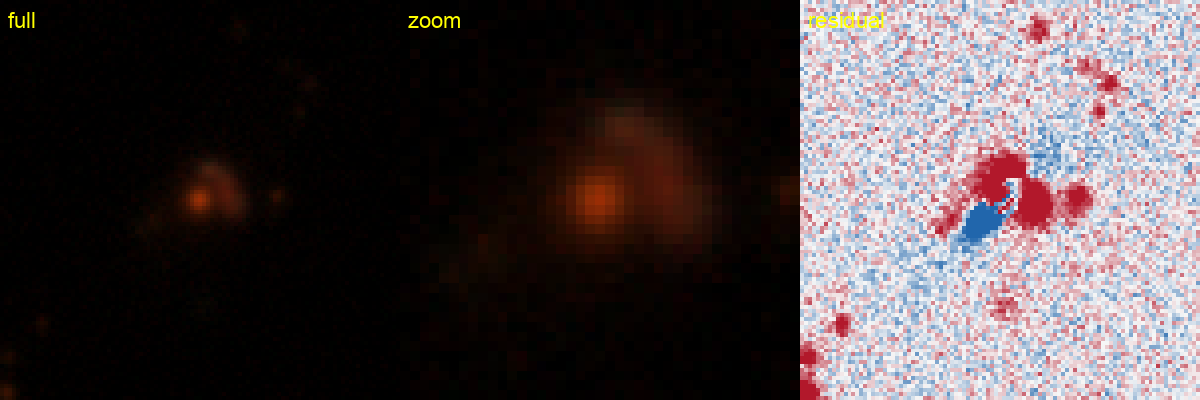
\includegraphics[width=\linewidth]{figures/res_s_129372_3768.png}
\caption{\textbf{\#73}~\texttt{s\_129372\_3768} --- RA 16.4504, Dec -37.4286; grade \textbf{B}, tier-1 $p_{\rm lens}$ 0.35, \vb{} 0.82. \textcolor{gray}{\textbf{KNOWN}} --- DES: \texttt{DES J010548.04-372542.4}, $0.71\arcsec$ (SIMBAD).}
\end{figure}
\begin{figure}[H]\centering
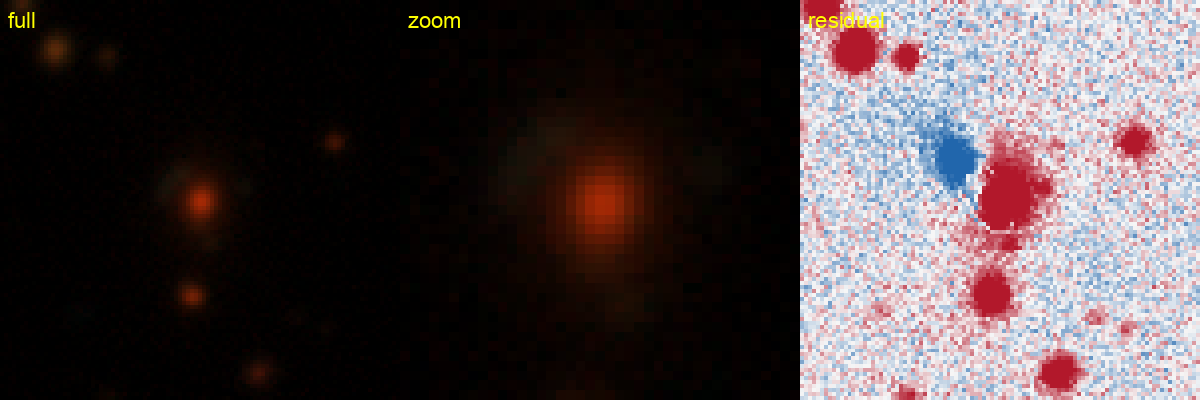
\includegraphics[width=\linewidth]{figures/res_s_238185_2253.png}
\caption{\textbf{\#74}~\texttt{s\_238185\_2253} --- RA 58.5761, Dec -16.1645; grade \textbf{B}, tier-1 $p_{\rm lens}$ 0.35, \vb{} 0.82. \textcolor{gray}{\textbf{KNOWN}} --- AGEL: \texttt{AGEL J035418-160952 system}, $0.51\arcsec$ (SIMBAD).}
\end{figure}
\begin{figure}[H]\centering
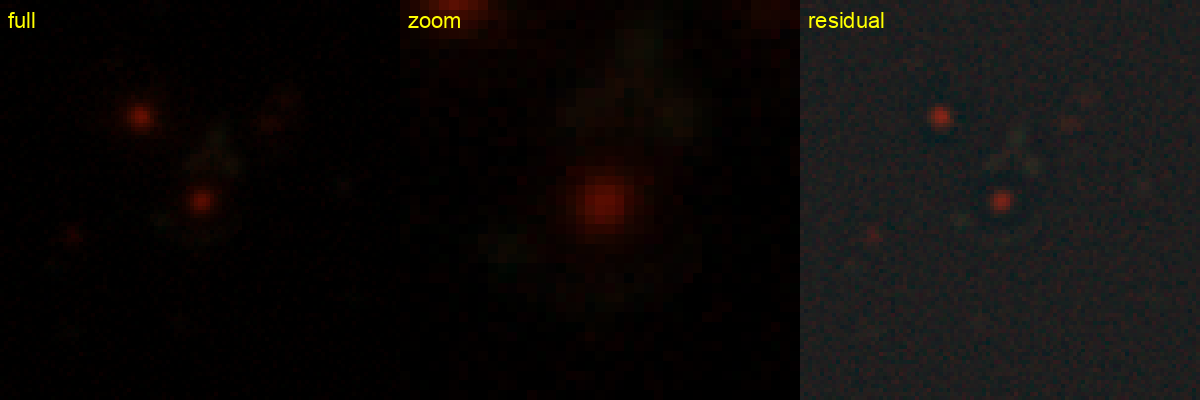
\includegraphics[width=\linewidth]{figures/res_s_94933_7964.png}
\caption{\textbf{\#75}~\texttt{s\_94933\_7964} --- RA 47.5548, Dec -45.5743; grade \textbf{B}, tier-1 $p_{\rm lens}$ 0.35, \vb{} 0.78. \textcolor{gray}{\textbf{KNOWN}} --- DES: \texttt{[DBL2017] DES J0310-4534 (A)}, $0.14\arcsec$ (SIMBAD).}
\end{figure}
\begin{figure}[H]\centering
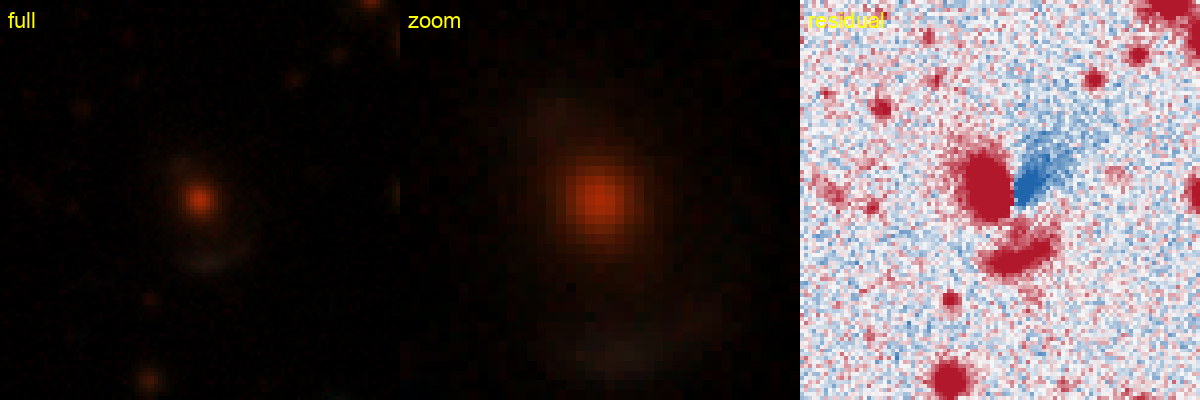
\includegraphics[width=\linewidth]{figures/res_s_71871_246.png}
\caption{\textbf{\#77}~\texttt{s\_71871\_246} --- RA 353.9664, Dec -51.8716; grade \textbf{B}, tier-1 $p_{\rm lens}$ 0.35, \vb{} 0.76. \textcolor{gray}{\textbf{KNOWN}} --- AGEL: \texttt{AGEL J233552-515218 system}, $0.95\arcsec$ (SIMBAD).}
\end{figure}
\begin{figure}[H]\centering
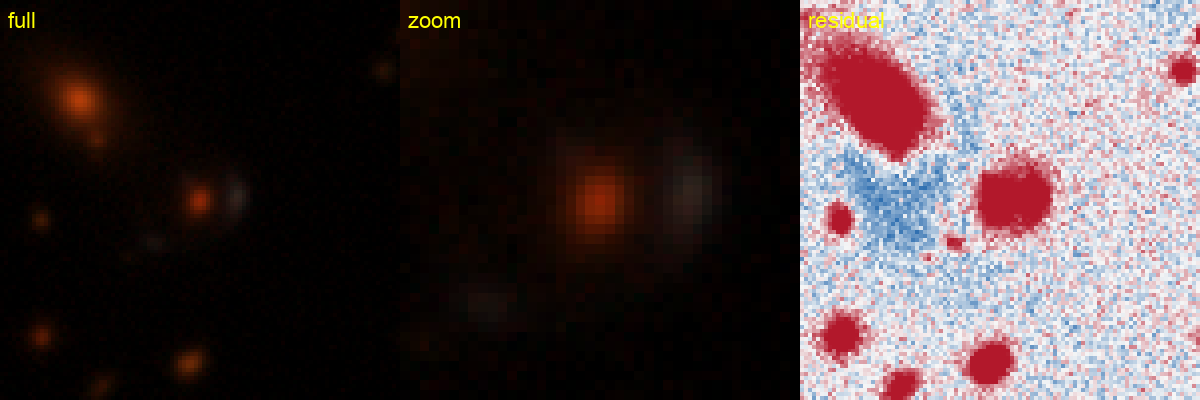
\includegraphics[width=\linewidth]{figures/res_s_90920_9419.png}
\caption{\textbf{\#78}~\texttt{s\_90920\_9419} --- RA 45.9517, Dec -46.4407; grade \textbf{B}, tier-1 $p_{\rm lens}$ 0.30, \vb{} 0.85. \textcolor{gray}{\textbf{KNOWN}} --- DES: \texttt{[DBL2017] DES J0303-4626 (A)}, $0.15\arcsec$ (SIMBAD).}
\end{figure}
\clearpage
\subsection*{\textcolor{forestgreen}{\textsc{New}} --- candidates new to the literature (25 of 78)}
These are absent from the DESI lens-finders, the DES/AGEL/CASSOWARY searches, and the NED/SIMBAD literature; all are grade~B, and at DECaLS $1\arcsec$ an unknown (likely large) fraction are lrg+companion mimics. Ranked by tier-1 $p_{\rm lens}$.\par\smallskip
\begin{figure}[H]\centering
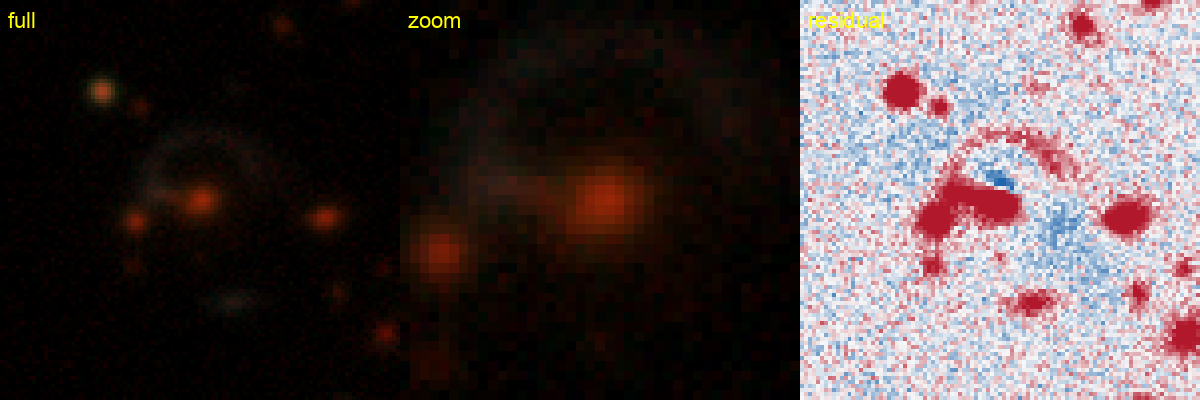
\includegraphics[width=\linewidth]{figures/res_s_230539_4159.png}
\caption{\textbf{\#9}~\texttt{s\_230539\_4159} --- RA 222.0715, Dec -17.8489; grade \textbf{B}, tier-1 $p_{\rm lens}$ 0.72, \vb{} 0.84. \textcolor{forestgreen}{\textbf{NEW}} --- new to the DESI lens-finders, the DES/AGEL/CASSOWARY searches, and the NED/SIMBAD literature.}
\end{figure}
\begin{figure}[H]\centering
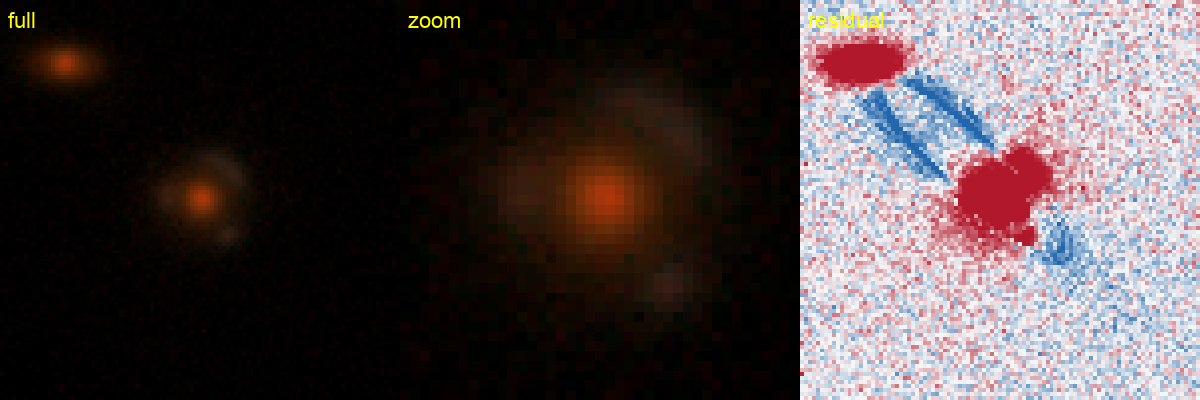
\includegraphics[width=\linewidth]{figures/res_s_234689_542.png}
\caption{\textbf{\#13}~\texttt{s\_234689\_542} --- RA 227.0427, Dec -16.8771; grade \textbf{B}, tier-1 $p_{\rm lens}$ 0.62, \vb{} 0.80. \textcolor{forestgreen}{\textbf{NEW}} --- new to the DESI lens-finders, the DES/AGEL/CASSOWARY searches, and the NED/SIMBAD literature.}
\end{figure}
\begin{figure}[H]\centering
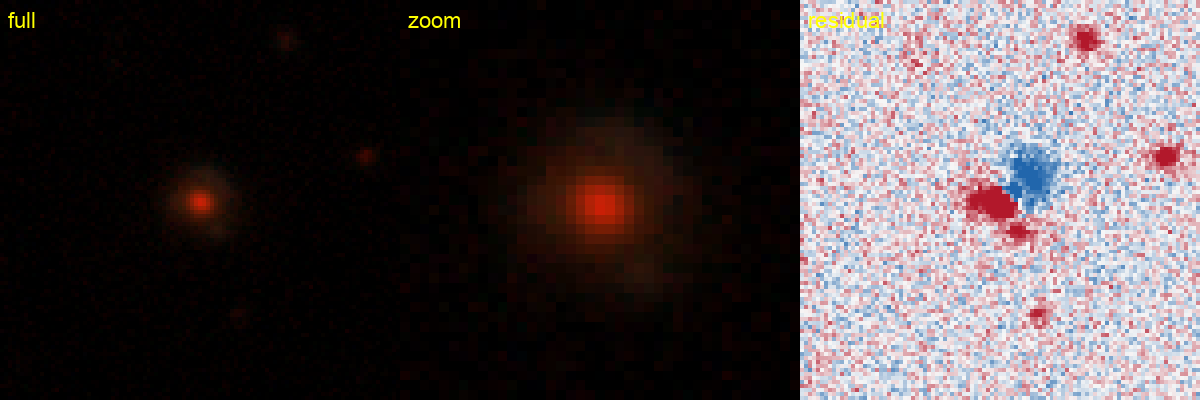
\includegraphics[width=\linewidth]{figures/res_s_205319_6061.png}
\caption{\textbf{\#15}~\texttt{s\_205319\_6061} --- RA 359.9772, Dec -22.4596; grade \textbf{B}, tier-1 $p_{\rm lens}$ 0.60, \vb{} 0.88. \textcolor{forestgreen}{\textbf{NEW}} --- new to the DESI lens-finders, the DES/AGEL/CASSOWARY searches, and the NED/SIMBAD literature.}
\end{figure}
\begin{figure}[H]\centering
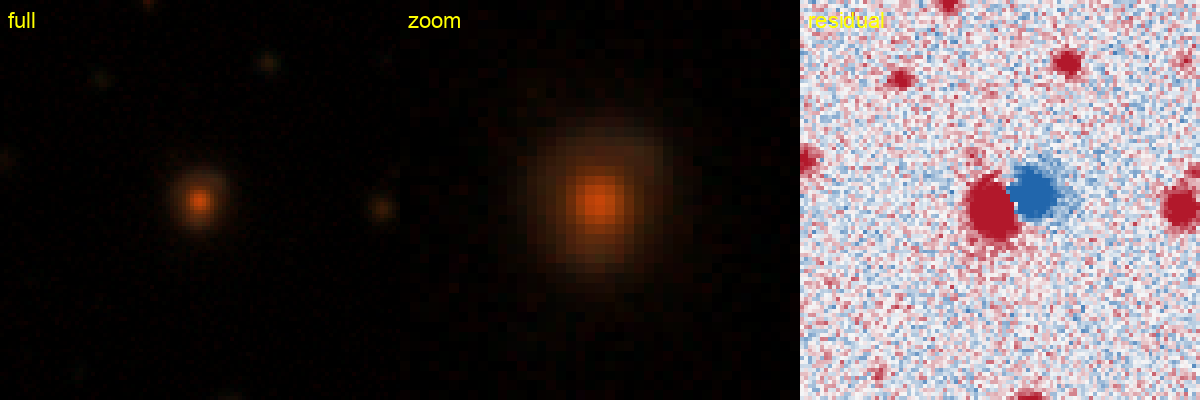
\includegraphics[width=\linewidth]{figures/res_s_218895_5088.png}
\caption{\textbf{\#18}~\texttt{s\_218895\_5088} --- RA 32.7525, Dec -19.6362; grade \textbf{B}, tier-1 $p_{\rm lens}$ 0.60, \vb{} 0.81. \textcolor{forestgreen}{\textbf{NEW}} --- new to the DESI lens-finders, the DES/AGEL/CASSOWARY searches, and the NED/SIMBAD literature.}
\end{figure}
\begin{figure}[H]\centering
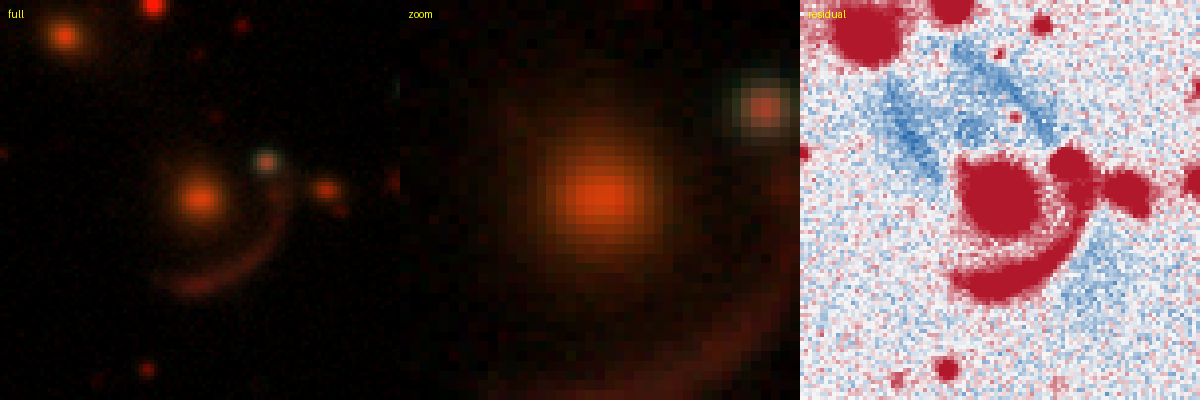
\includegraphics[width=\linewidth]{figures/res_s_194300_2796.png}
\caption{\textbf{\#22}~\texttt{s\_194300\_2796} --- RA 242.6052, Dec -24.4155; grade \textbf{B}, tier-1 $p_{\rm lens}$ 0.58, \vb{} 0.74. \textcolor{forestgreen}{\textbf{NEW}} --- new to the DESI lens-finders, the DES/AGEL/CASSOWARY searches, and the NED/SIMBAD literature.}
\end{figure}
\begin{figure}[H]\centering
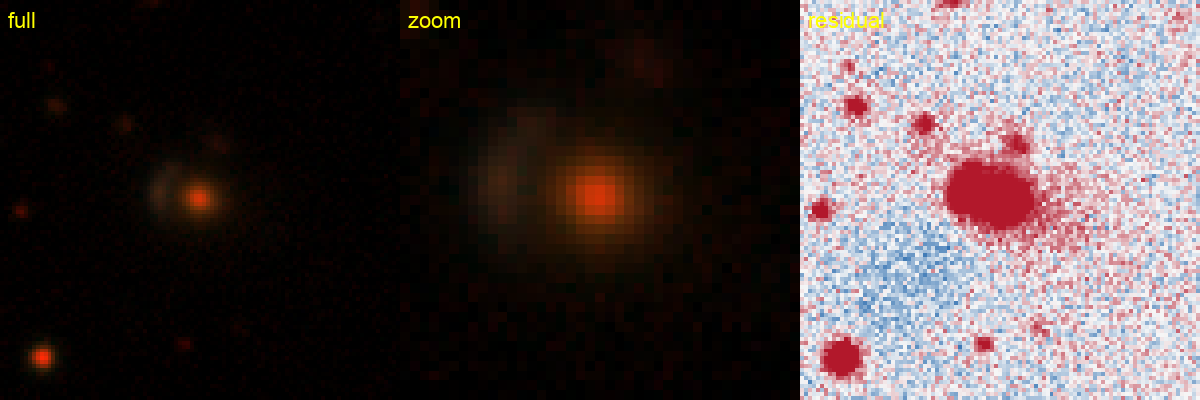
\includegraphics[width=\linewidth]{figures/res_s_23764_4161.png}
\caption{\textbf{\#28}~\texttt{s\_23764\_4161} --- RA 132.6603, Dec -68.1876; grade \textbf{B}, tier-1 $p_{\rm lens}$ 0.55, \vb{} 0.79. \textcolor{forestgreen}{\textbf{NEW}} --- new to the DESI lens-finders, the DES/AGEL/CASSOWARY searches, and the NED/SIMBAD literature.}
\end{figure}
\begin{figure}[H]\centering
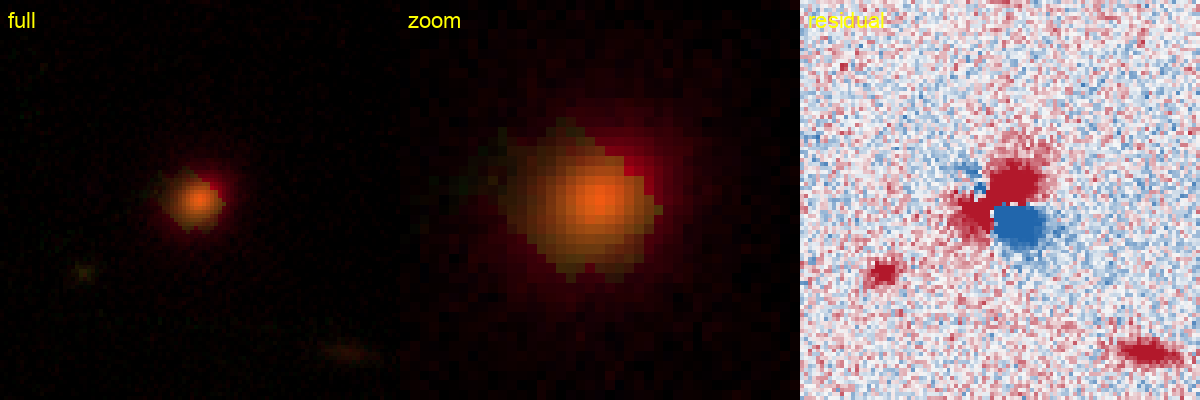
\includegraphics[width=\linewidth]{figures/res_s_353585_141.png}
\caption{\textbf{\#32}~\texttt{s\_353585\_141} --- RA 45.8222, Dec +3.9613; grade \textbf{B}, tier-1 $p_{\rm lens}$ 0.50, \vb{} 0.84. \textcolor{forestgreen}{\textbf{NEW}} --- new to the DESI lens-finders, the DES/AGEL/CASSOWARY searches, and the NED/SIMBAD literature.}
\end{figure}
\begin{figure}[H]\centering
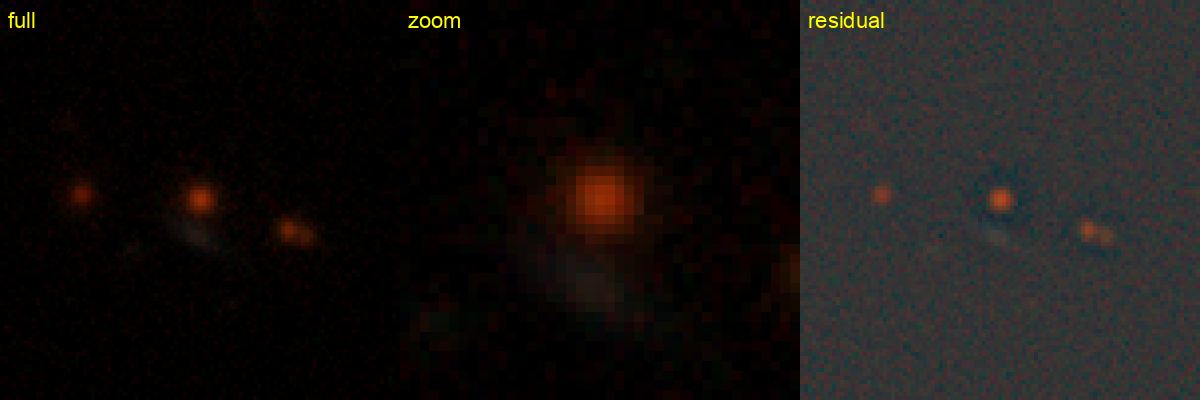
\includegraphics[width=\linewidth]{figures/res_s_289350_3716.png}
\caption{\textbf{\#35}~\texttt{s\_289350\_3716} --- RA 164.8051, Dec -7.1449; grade \textbf{B}, tier-1 $p_{\rm lens}$ 0.50, \vb{} 0.81. \textcolor{forestgreen}{\textbf{NEW}} --- new to the DESI lens-finders, the DES/AGEL/CASSOWARY searches, and the NED/SIMBAD literature.}
\end{figure}
\begin{figure}[H]\centering
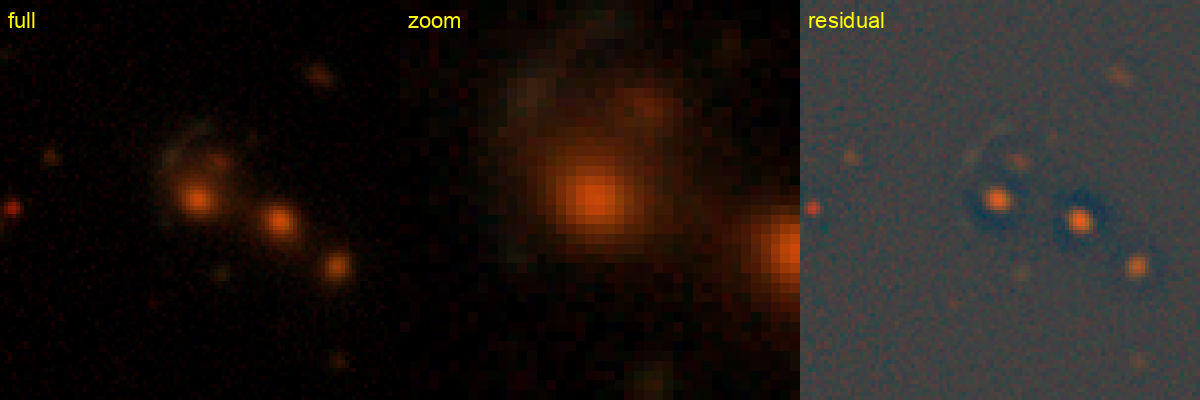
\includegraphics[width=\linewidth]{figures/res_s_148704_6732.png}
\caption{\textbf{\#36}~\texttt{s\_148704\_6732} --- RA 183.8176, Dec -33.6006; grade \textbf{B}, tier-1 $p_{\rm lens}$ 0.50, \vb{} 0.80. \textcolor{forestgreen}{\textbf{NEW}} --- new to the DESI lens-finders, the DES/AGEL/CASSOWARY searches, and the NED/SIMBAD literature.}
\end{figure}
\begin{figure}[H]\centering
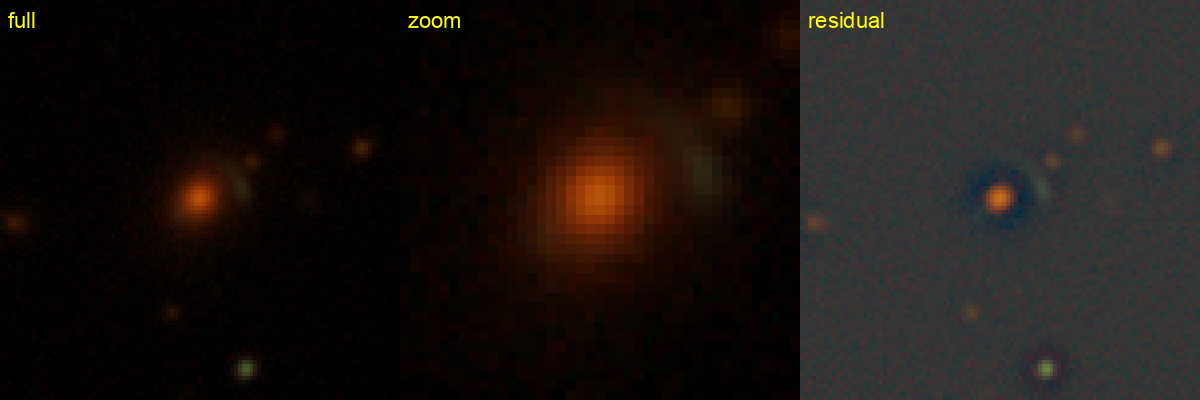
\includegraphics[width=\linewidth]{figures/res_s_90098_8002.png}
\caption{\textbf{\#41}~\texttt{s\_90098\_8002} --- RA 107.1696, Dec -46.7832; grade \textbf{B}, tier-1 $p_{\rm lens}$ 0.45, \vb{} 0.83. \textcolor{forestgreen}{\textbf{NEW}} --- new to the DESI lens-finders, the DES/AGEL/CASSOWARY searches, and the NED/SIMBAD literature.}
\end{figure}
\begin{figure}[H]\centering
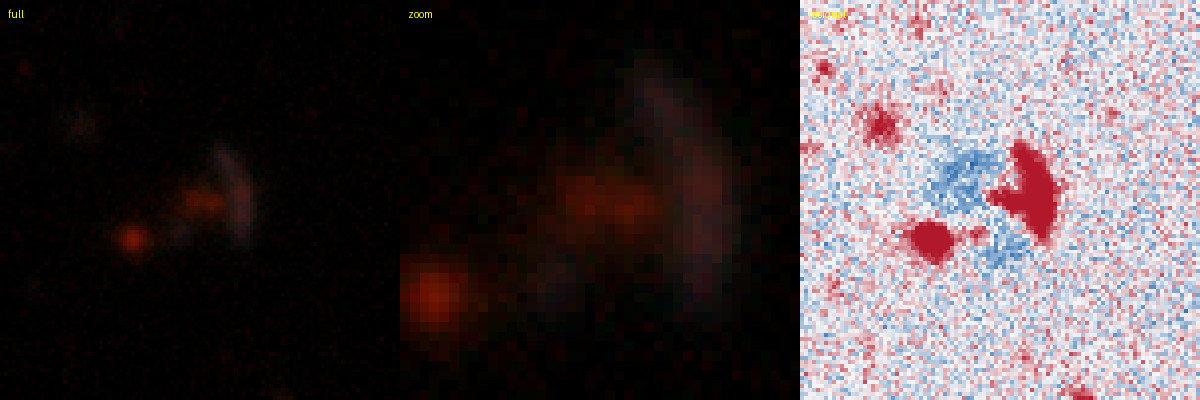
\includegraphics[width=\linewidth]{figures/res_s_502450_1680.png}
\caption{\textbf{\#43}~\texttt{s\_502450\_1680} --- RA 161.1145, Dec +31.2344; grade \textbf{B}, tier-1 $p_{\rm lens}$ 0.45, \vb{} 0.79. \textcolor{forestgreen}{\textbf{NEW}} --- new to the DESI lens-finders, the DES/AGEL/CASSOWARY searches, and the NED/SIMBAD literature.}
\end{figure}
\begin{figure}[H]\centering
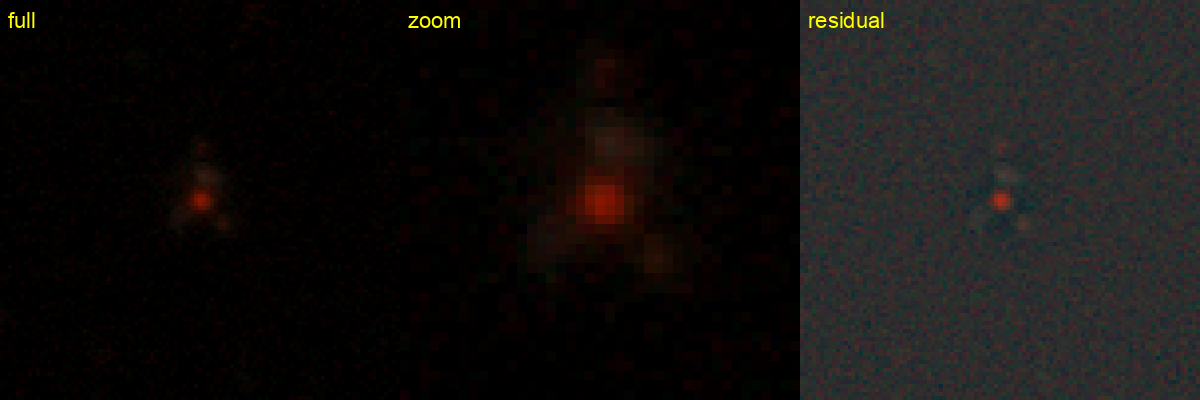
\includegraphics[width=\linewidth]{figures/res_s_426295_4804.png}
\caption{\textbf{\#44}~\texttt{s\_426295\_4804} --- RA 182.0229, Dec +16.6326; grade \textbf{B}, tier-1 $p_{\rm lens}$ 0.45, \vb{} 0.79. \textcolor{forestgreen}{\textbf{NEW}} --- new to the DESI lens-finders, the DES/AGEL/CASSOWARY searches, and the NED/SIMBAD literature.}
\end{figure}
\begin{figure}[H]\centering
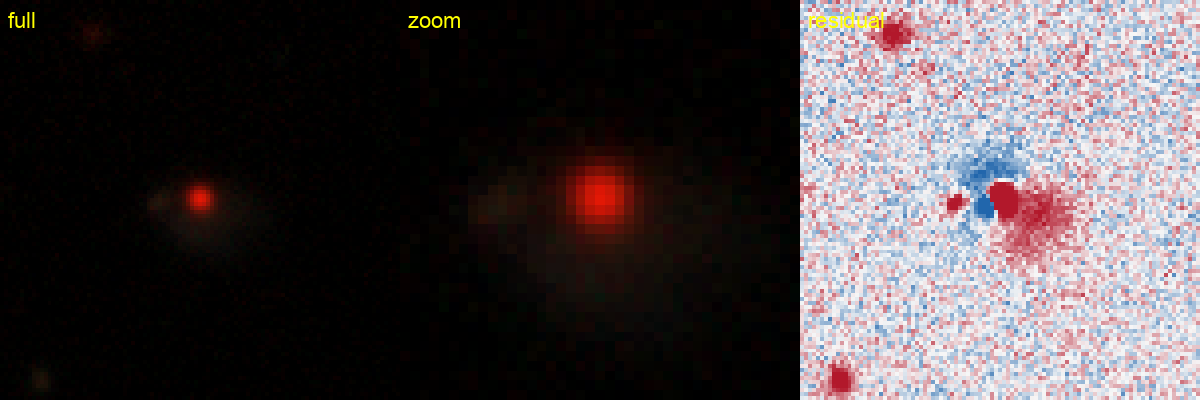
\includegraphics[width=\linewidth]{figures/res_s_369309_653.png}
\caption{\textbf{\#45}~\texttt{s\_369309\_653} --- RA 30.4465, Dec +6.6551; grade \textbf{B}, tier-1 $p_{\rm lens}$ 0.45, \vb{} 0.74. \textcolor{forestgreen}{\textbf{NEW}} --- new to the DESI lens-finders, the DES/AGEL/CASSOWARY searches, and the NED/SIMBAD literature.}
\end{figure}
\begin{figure}[H]\centering
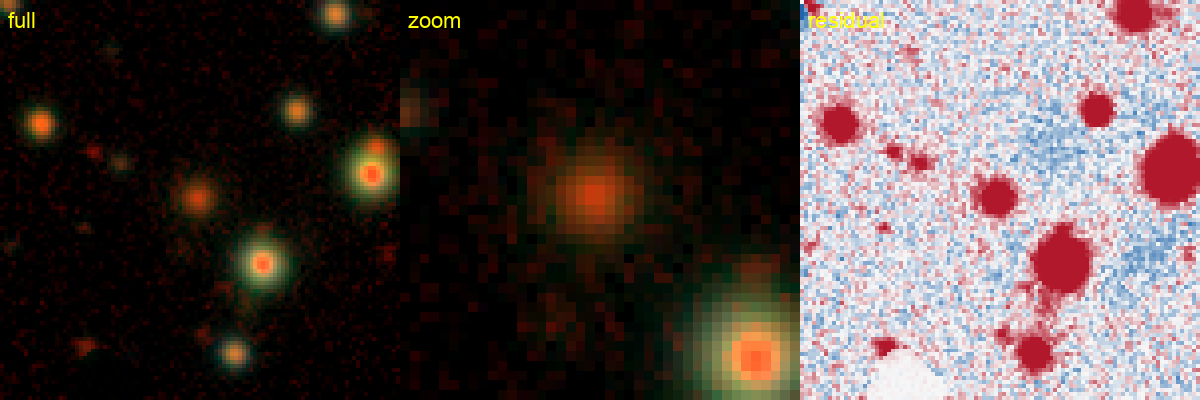
\includegraphics[width=\linewidth]{figures/res_s_32666_26056.png}
\caption{\textbf{\#46}~\texttt{s\_32666\_26056} --- RA 248.6090, Dec -64.5569; grade \textbf{B}, tier-1 $p_{\rm lens}$ 0.45, \vb{} 0.73. \textcolor{forestgreen}{\textbf{NEW}} --- new to the DESI lens-finders, the DES/AGEL/CASSOWARY searches, and the NED/SIMBAD literature.}
\end{figure}
\begin{figure}[H]\centering
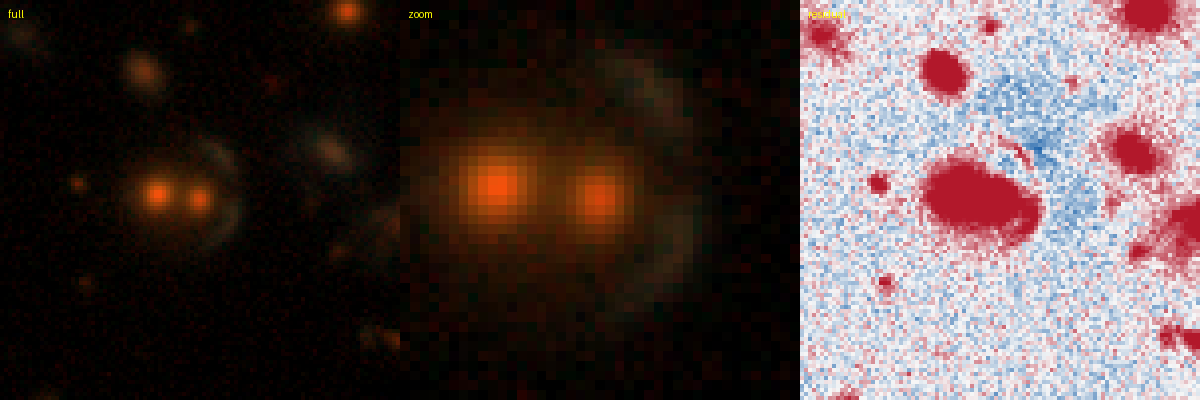
\includegraphics[width=\linewidth]{figures/res_s_266620_918.png}
\caption{\textbf{\#52}~\texttt{s\_266620\_918} --- RA 172.1320, Dec -11.3108; grade \textbf{B}, tier-1 $p_{\rm lens}$ 0.42, \vb{} 0.80. \textcolor{forestgreen}{\textbf{NEW}} --- new to the DESI lens-finders, the DES/AGEL/CASSOWARY searches, and the NED/SIMBAD literature.}
\end{figure}
\begin{figure}[H]\centering
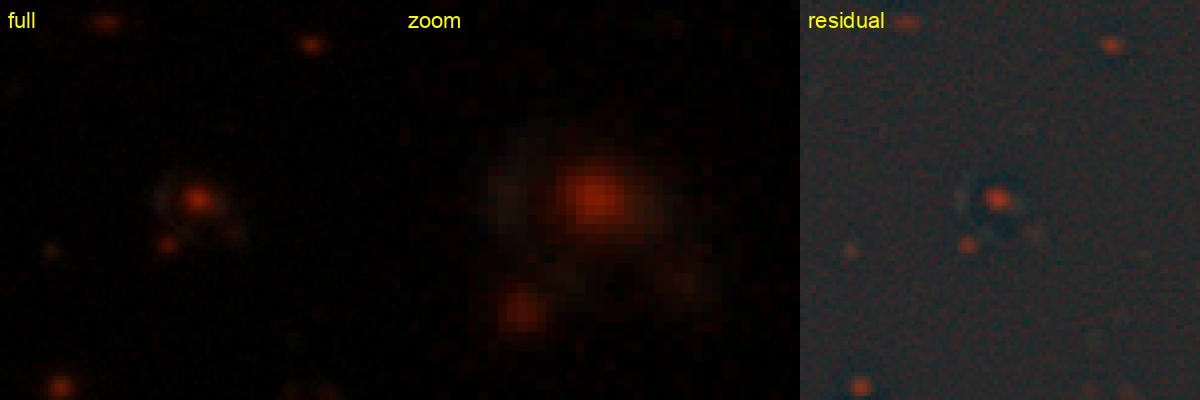
\includegraphics[width=\linewidth]{figures/res_s_242312_4967.png}
\caption{\textbf{\#53}~\texttt{s\_242312\_4967} --- RA 50.3567, Dec -15.5010; grade \textbf{B}, tier-1 $p_{\rm lens}$ 0.40, \vb{} 0.90. \textcolor{forestgreen}{\textbf{NEW}} --- new to the DESI lens-finders, the DES/AGEL/CASSOWARY searches, and the NED/SIMBAD literature.}
\end{figure}
\begin{figure}[H]\centering
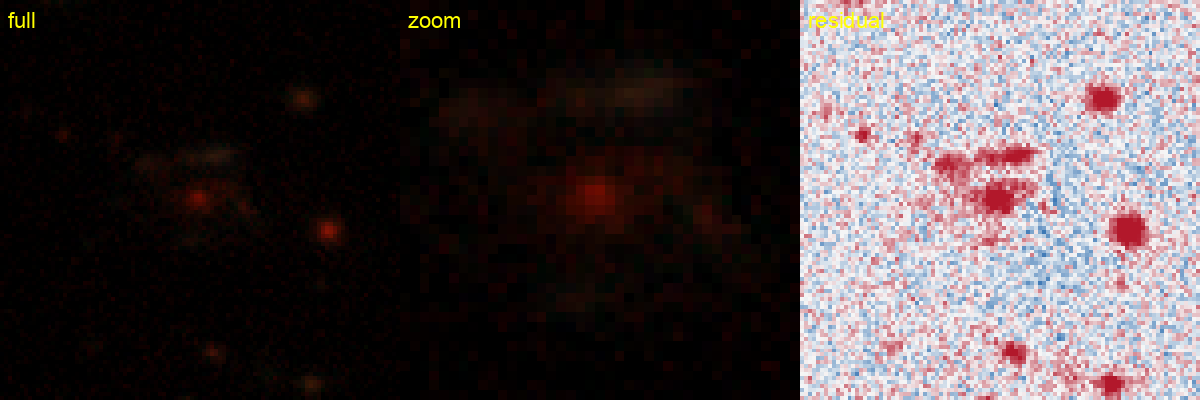
\includegraphics[width=\linewidth]{figures/res_s_262449_2840.png}
\caption{\textbf{\#56}~\texttt{s\_262449\_2840} --- RA 188.7861, Dec -11.9798; grade \textbf{B}, tier-1 $p_{\rm lens}$ 0.40, \vb{} 0.87. \textcolor{forestgreen}{\textbf{NEW}} --- new to the DESI lens-finders, the DES/AGEL/CASSOWARY searches, and the NED/SIMBAD literature.}
\end{figure}
\begin{figure}[H]\centering
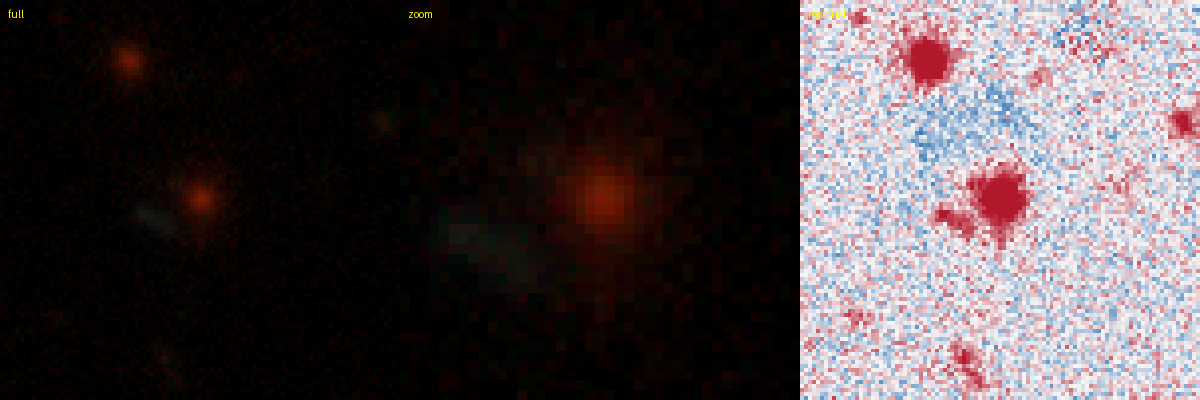
\includegraphics[width=\linewidth]{figures/res_s_360639_3636.png}
\caption{\textbf{\#58}~\texttt{s\_360639\_3636} --- RA 13.4868, Dec +5.3590; grade \textbf{B}, tier-1 $p_{\rm lens}$ 0.40, \vb{} 0.85. \textcolor{forestgreen}{\textbf{NEW}} --- new to the DESI lens-finders, the DES/AGEL/CASSOWARY searches, and the NED/SIMBAD literature.}
\end{figure}
\begin{figure}[H]\centering
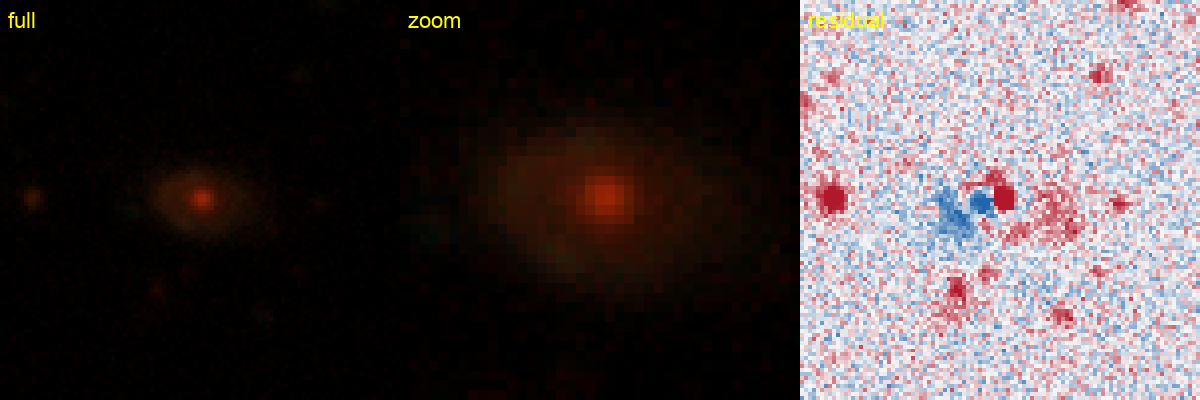
\includegraphics[width=\linewidth]{figures/res_s_188312_3322.png}
\caption{\textbf{\#64}~\texttt{s\_188312\_3322} --- RA 33.2537, Dec -25.3945; grade \textbf{B}, tier-1 $p_{\rm lens}$ 0.40, \vb{} 0.76. \textcolor{forestgreen}{\textbf{NEW}} --- new to the DESI lens-finders, the DES/AGEL/CASSOWARY searches, and the NED/SIMBAD literature.}
\end{figure}
\begin{figure}[H]\centering
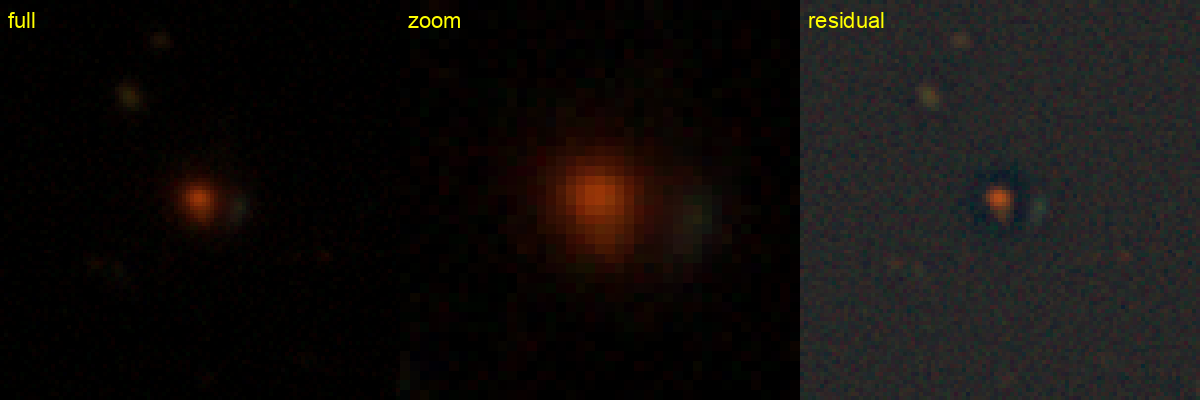
\includegraphics[width=\linewidth]{figures/res_s_188754_2468.png}
\caption{\textbf{\#65}~\texttt{s\_188754\_2468} --- RA 155.4695, Dec -25.5029; grade \textbf{B}, tier-1 $p_{\rm lens}$ 0.40, \vb{} 0.74. \textcolor{forestgreen}{\textbf{NEW}} --- new to the DESI lens-finders, the DES/AGEL/CASSOWARY searches, and the NED/SIMBAD literature.}
\end{figure}
\begin{figure}[H]\centering
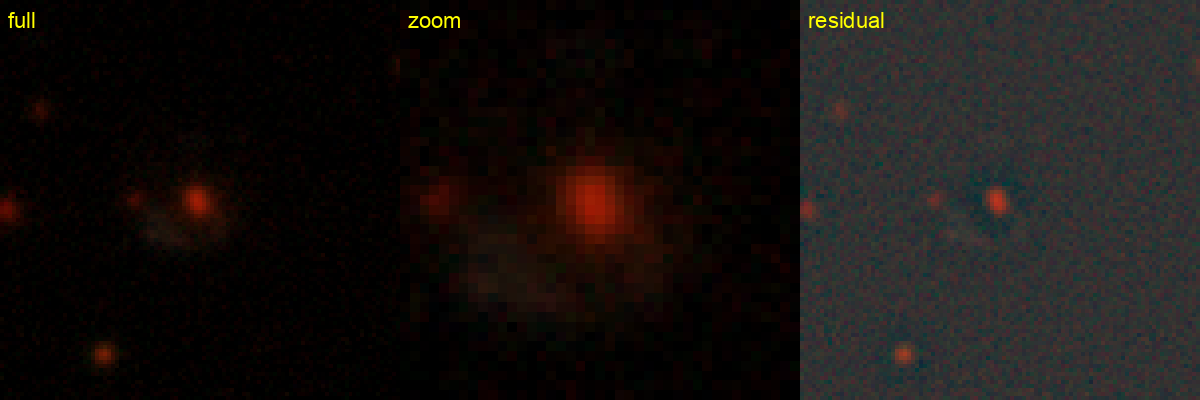
\includegraphics[width=\linewidth]{figures/res_s_405220_1292.png}
\caption{\textbf{\#67}~\texttt{s\_405220\_1292} --- RA 136.4655, Dec +13.0307; grade \textbf{B}, tier-1 $p_{\rm lens}$ 0.38, \vb{} 0.89. \textcolor{forestgreen}{\textbf{NEW}} --- new to the DESI lens-finders, the DES/AGEL/CASSOWARY searches, and the NED/SIMBAD literature.}
\end{figure}
\begin{figure}[H]\centering
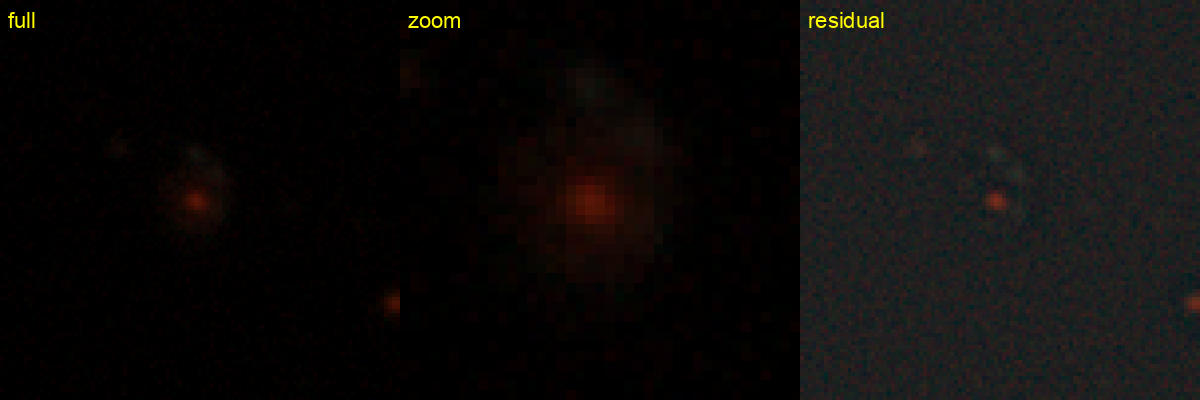
\includegraphics[width=\linewidth]{figures/res_s_250611_2161.png}
\caption{\textbf{\#70}~\texttt{s\_250611\_2161} --- RA 33.7898, Dec -14.1185; grade \textbf{B}, tier-1 $p_{\rm lens}$ 0.38, \vb{} 0.77. \textcolor{forestgreen}{\textbf{NEW}} --- new to the DESI lens-finders, the DES/AGEL/CASSOWARY searches, and the NED/SIMBAD literature.}
\end{figure}
\begin{figure}[H]\centering
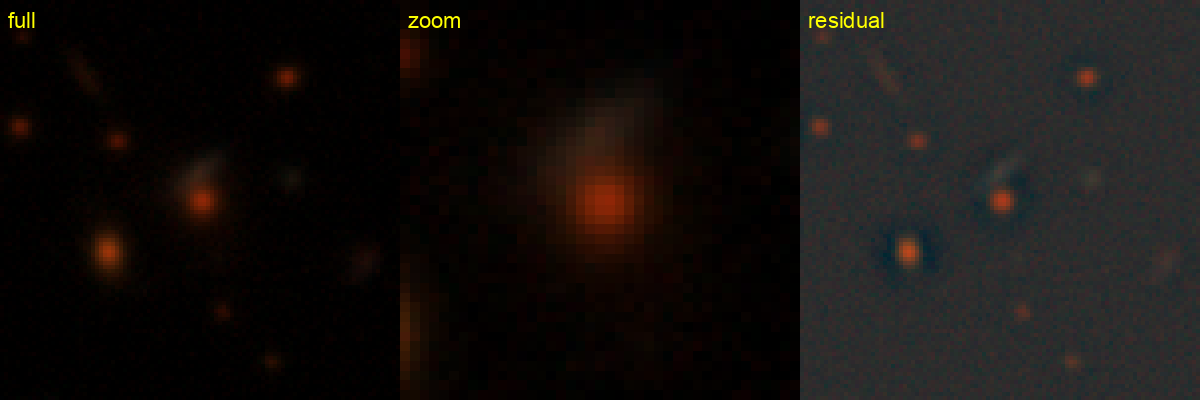
\includegraphics[width=\linewidth]{figures/res_s_161725_5181.png}
\caption{\textbf{\#71}~\texttt{s\_161725\_5181} --- RA 61.4085, Dec -30.6887; grade \textbf{B}, tier-1 $p_{\rm lens}$ 0.38, \vb{} 0.76. \textcolor{forestgreen}{\textbf{NEW}} --- new to the DESI lens-finders, the DES/AGEL/CASSOWARY searches, and the NED/SIMBAD literature.}
\end{figure}
\begin{figure}[H]\centering
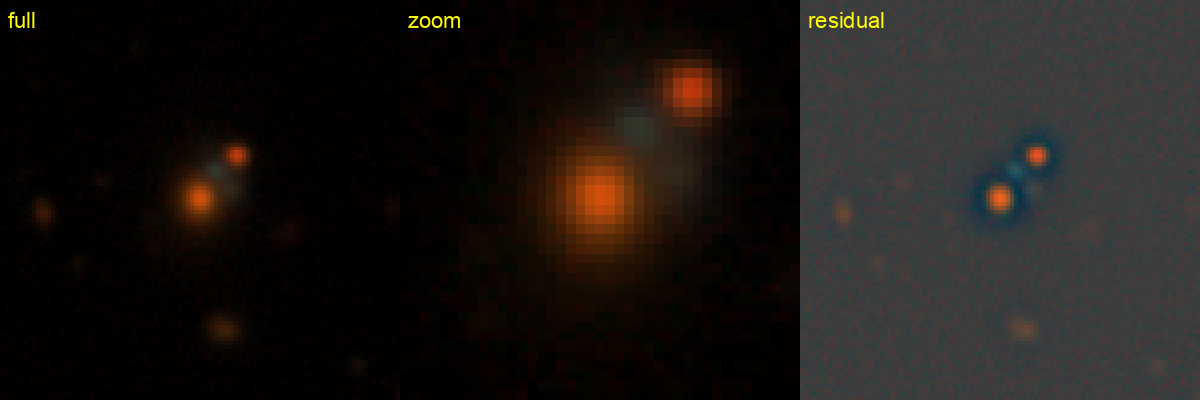
\includegraphics[width=\linewidth]{figures/res_s_210799_616.png}
\caption{\textbf{\#72}~\texttt{s\_210799\_616} --- RA 33.4979, Dec -21.2827; grade \textbf{B}, tier-1 $p_{\rm lens}$ 0.38, \vb{} 0.75. \textcolor{forestgreen}{\textbf{NEW}} --- new to the DESI lens-finders, the DES/AGEL/CASSOWARY searches, and the NED/SIMBAD literature.}
\end{figure}
\begin{figure}[H]\centering
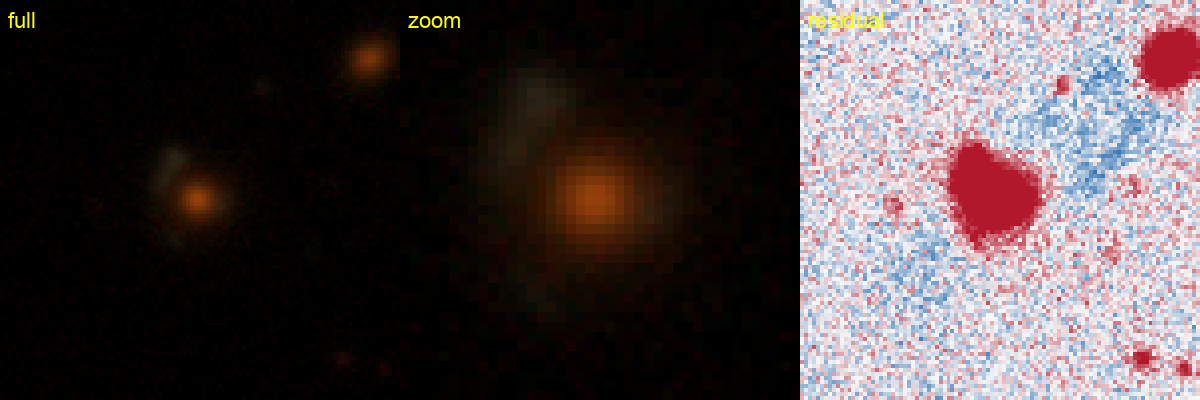
\includegraphics[width=\linewidth]{figures/res_s_250997_4626.png}
\caption{\textbf{\#76}~\texttt{s\_250997\_4626} --- RA 133.2708, Dec -13.8944; grade \textbf{B}, tier-1 $p_{\rm lens}$ 0.35, \vb{} 0.77. \textcolor{forestgreen}{\textbf{NEW}} --- new to the DESI lens-finders, the DES/AGEL/CASSOWARY searches, and the NED/SIMBAD literature.}
\end{figure}

\end{document}
